\section{安定化制御実験}
	振子を上向きに配置したときに安定化制御が可能か実験を行う。(実験目的の第一項目)
	その際に、振子を真上に配置するのではなく、幾分か角度をつけてから実験を始める。
	実験に用いたパラメータを以下の表に示す。
	\begin{table}[H]
		\begin{center}
			\caption{安定化制御実験で使用したパラメータの組}
			\medskip
			
			\begin{tabular}{|c|c|c|c|}\hline
				重み行列$Q$ & オブザーバの極$P$ & サンプリング周期$\Delta[\rm{s}]$ \\ \hline\hline
				$Q_1$:$\rm{diag}(1E5,1E5,1,1)$ & $P_1$:$((-30,0),(-30,0))^{'}$ & $\Delta_1$:0.005 \\ \hline
			\end{tabular}
		\end{center}
		\label{table:huriage_control}
	\end{table}
	以下に実験結果とシミュレーション結果の比較した図を示す。
	\begin{figure}[H]
		\centering
		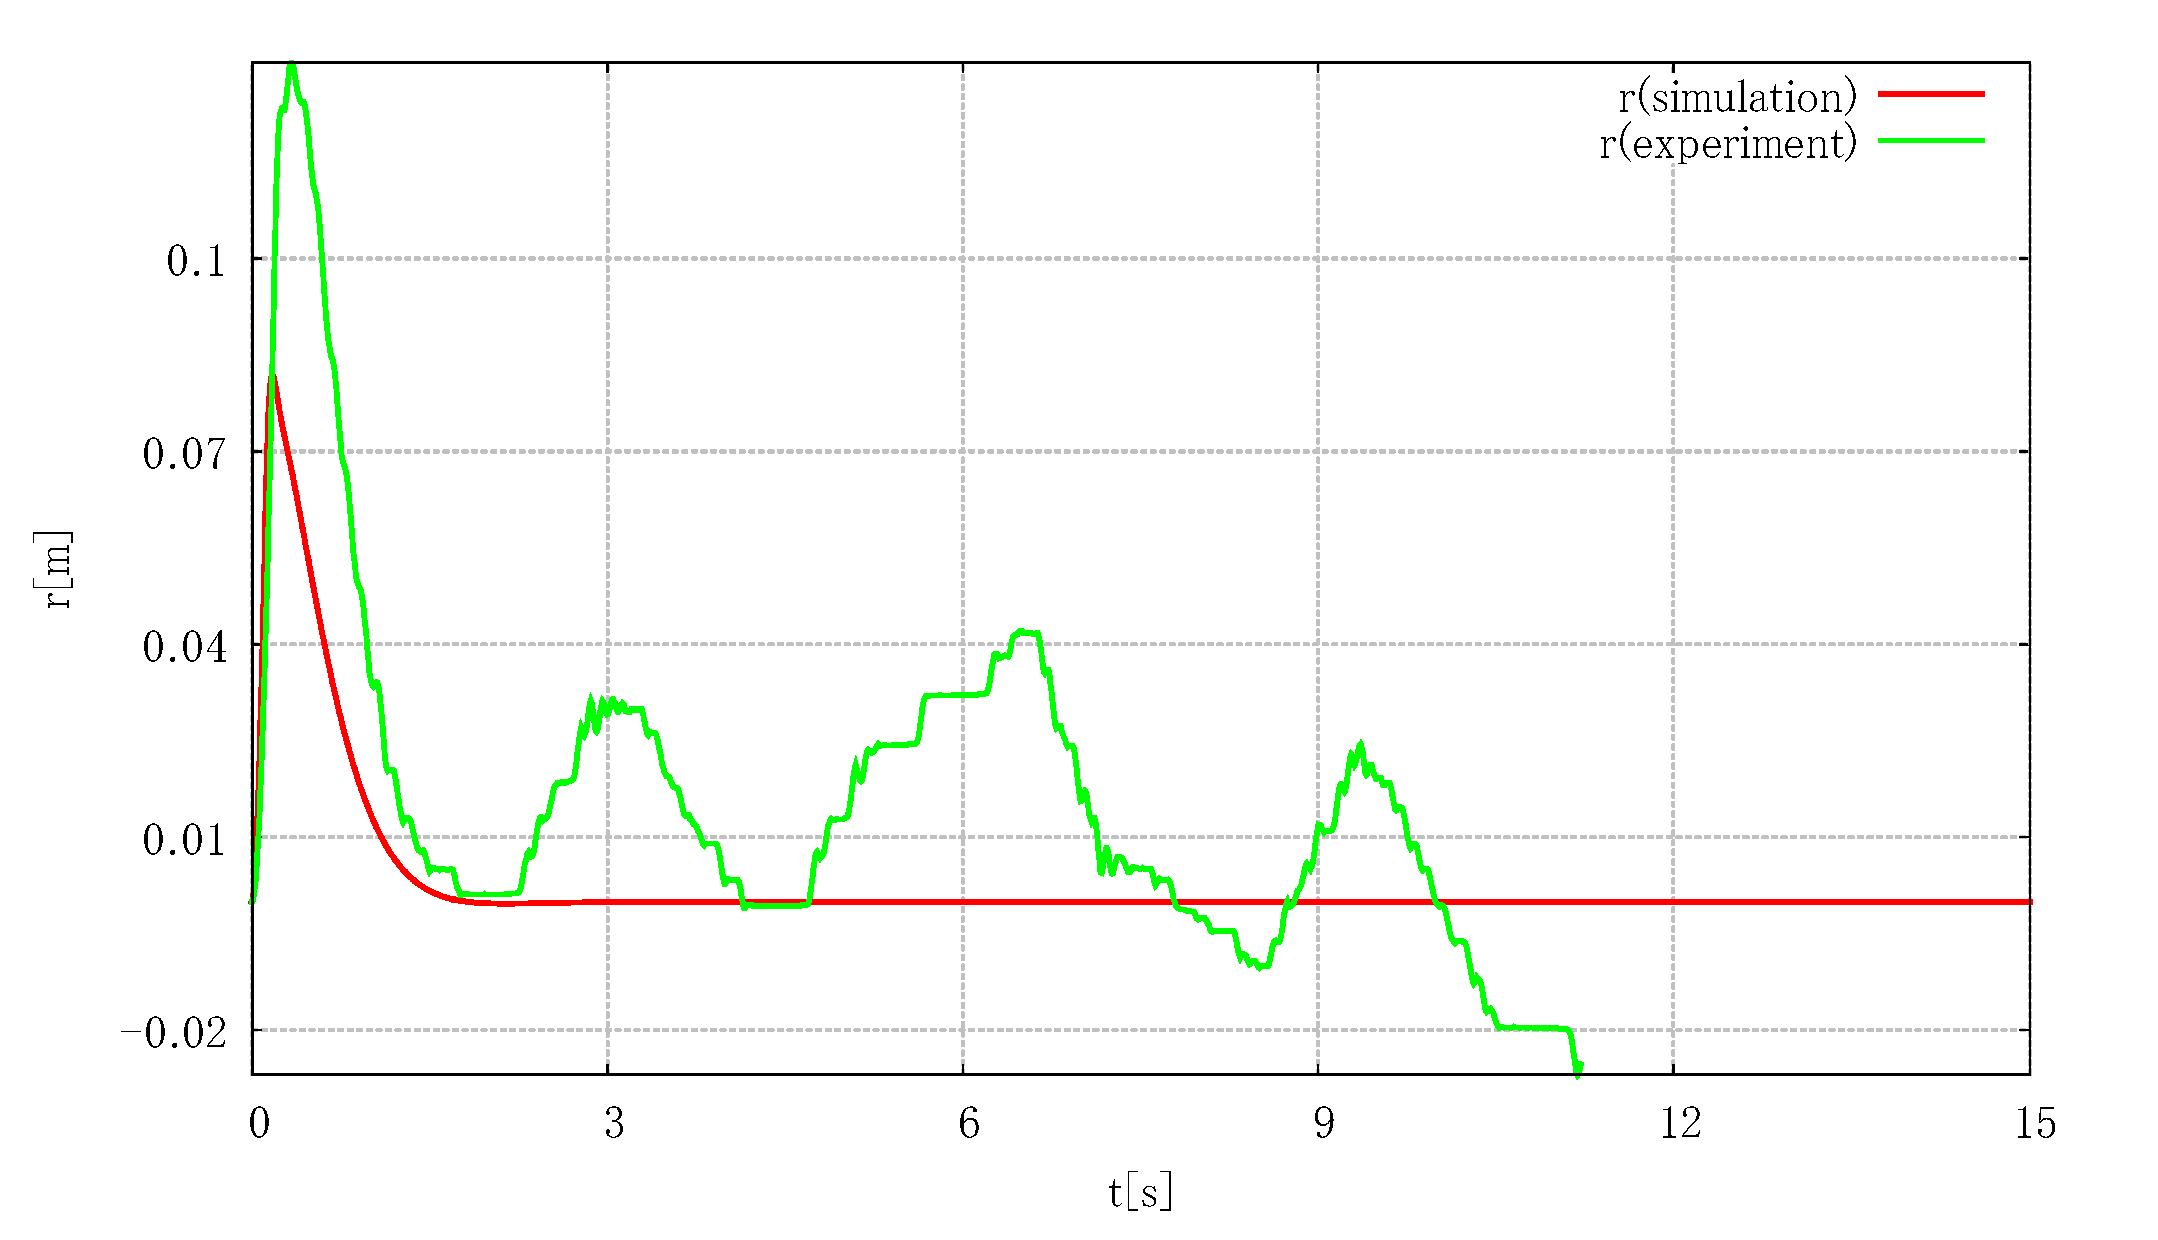
\includegraphics[width=0.8\linewidth]{gazo/experiment_control_R.eps}
		\caption{安定化制御実験結果(台車位置)}
		\label{image:experiment_control_R}
	\end{figure}
	\begin{figure}[H]
		\centering
		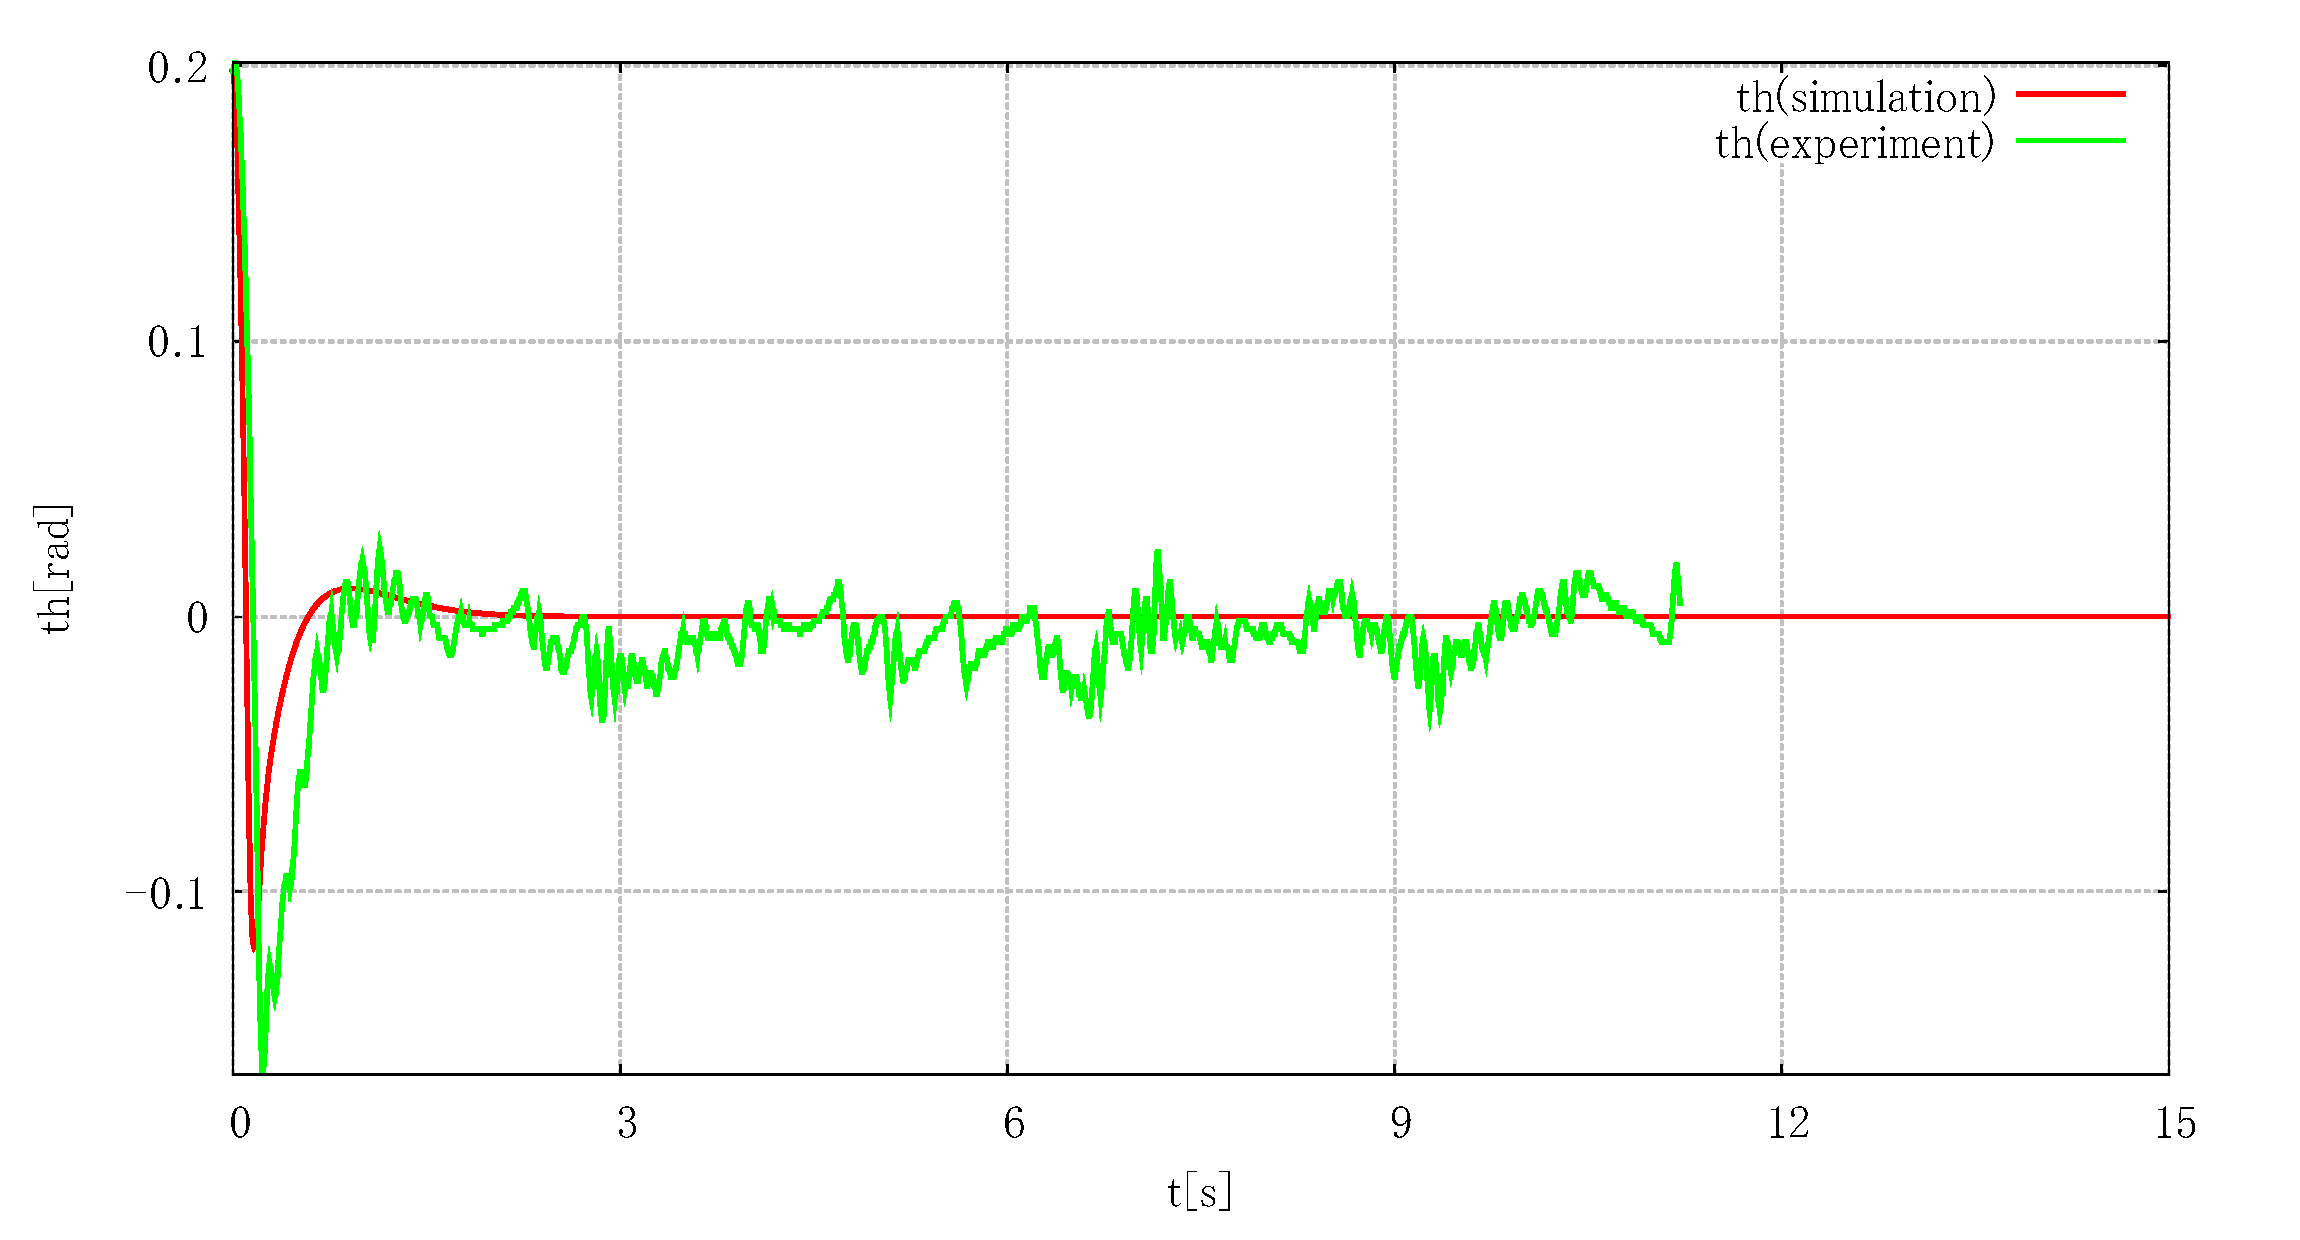
\includegraphics[width=0.8\linewidth]{gazo/experiment_control_TH.eps}
		\caption{安定化制御実験結果(振子角度)}
		\label{image:experiment_control_TH}
	\end{figure}
	図\ref{image:experiment_control_R}と図\ref{image:experiment_control_TH}
	より一番最初の山は実験のほうが大幅に大きくなっているのと、ノイズが乗っている点を除いてシミュレーションと実験結果は
	概ね一致しているといえる。これは、実験のほうではデータの計測を開始して振子から手を離したためその影響が出たといえる。
	この時の初期角度は$11.34°$である。%radに直してほしいなぁ
	よって、初期角度がある程度ある中で実験を開始し、安定化制御を行うことができたため、
	実験目的の第一項目を達成できたといえる。
	
	
	
%-----------------------------------------------------------
\newpage
\section{目標値の変更実験}
	台車に目標値を与えて、その目標値に台車が移動しても安定化制御可能か実験を行う。(実験項目の第二項目)
	なお、目標値は5秒ごとに0→0.1→0のように変更される。
	以下に、重み行列を変更した場合の比較、オブザーバの極を変更した場合の比較、サンプリング周期を変更した場合の比較を
	行った図を示す。
	\par
	\subsection{重み行列の違いによる実験結果の比較}
	最初に重み行列を変更した場合の実験結果の比較を見てみる。
	\begin{figure}[H]
		\centering
		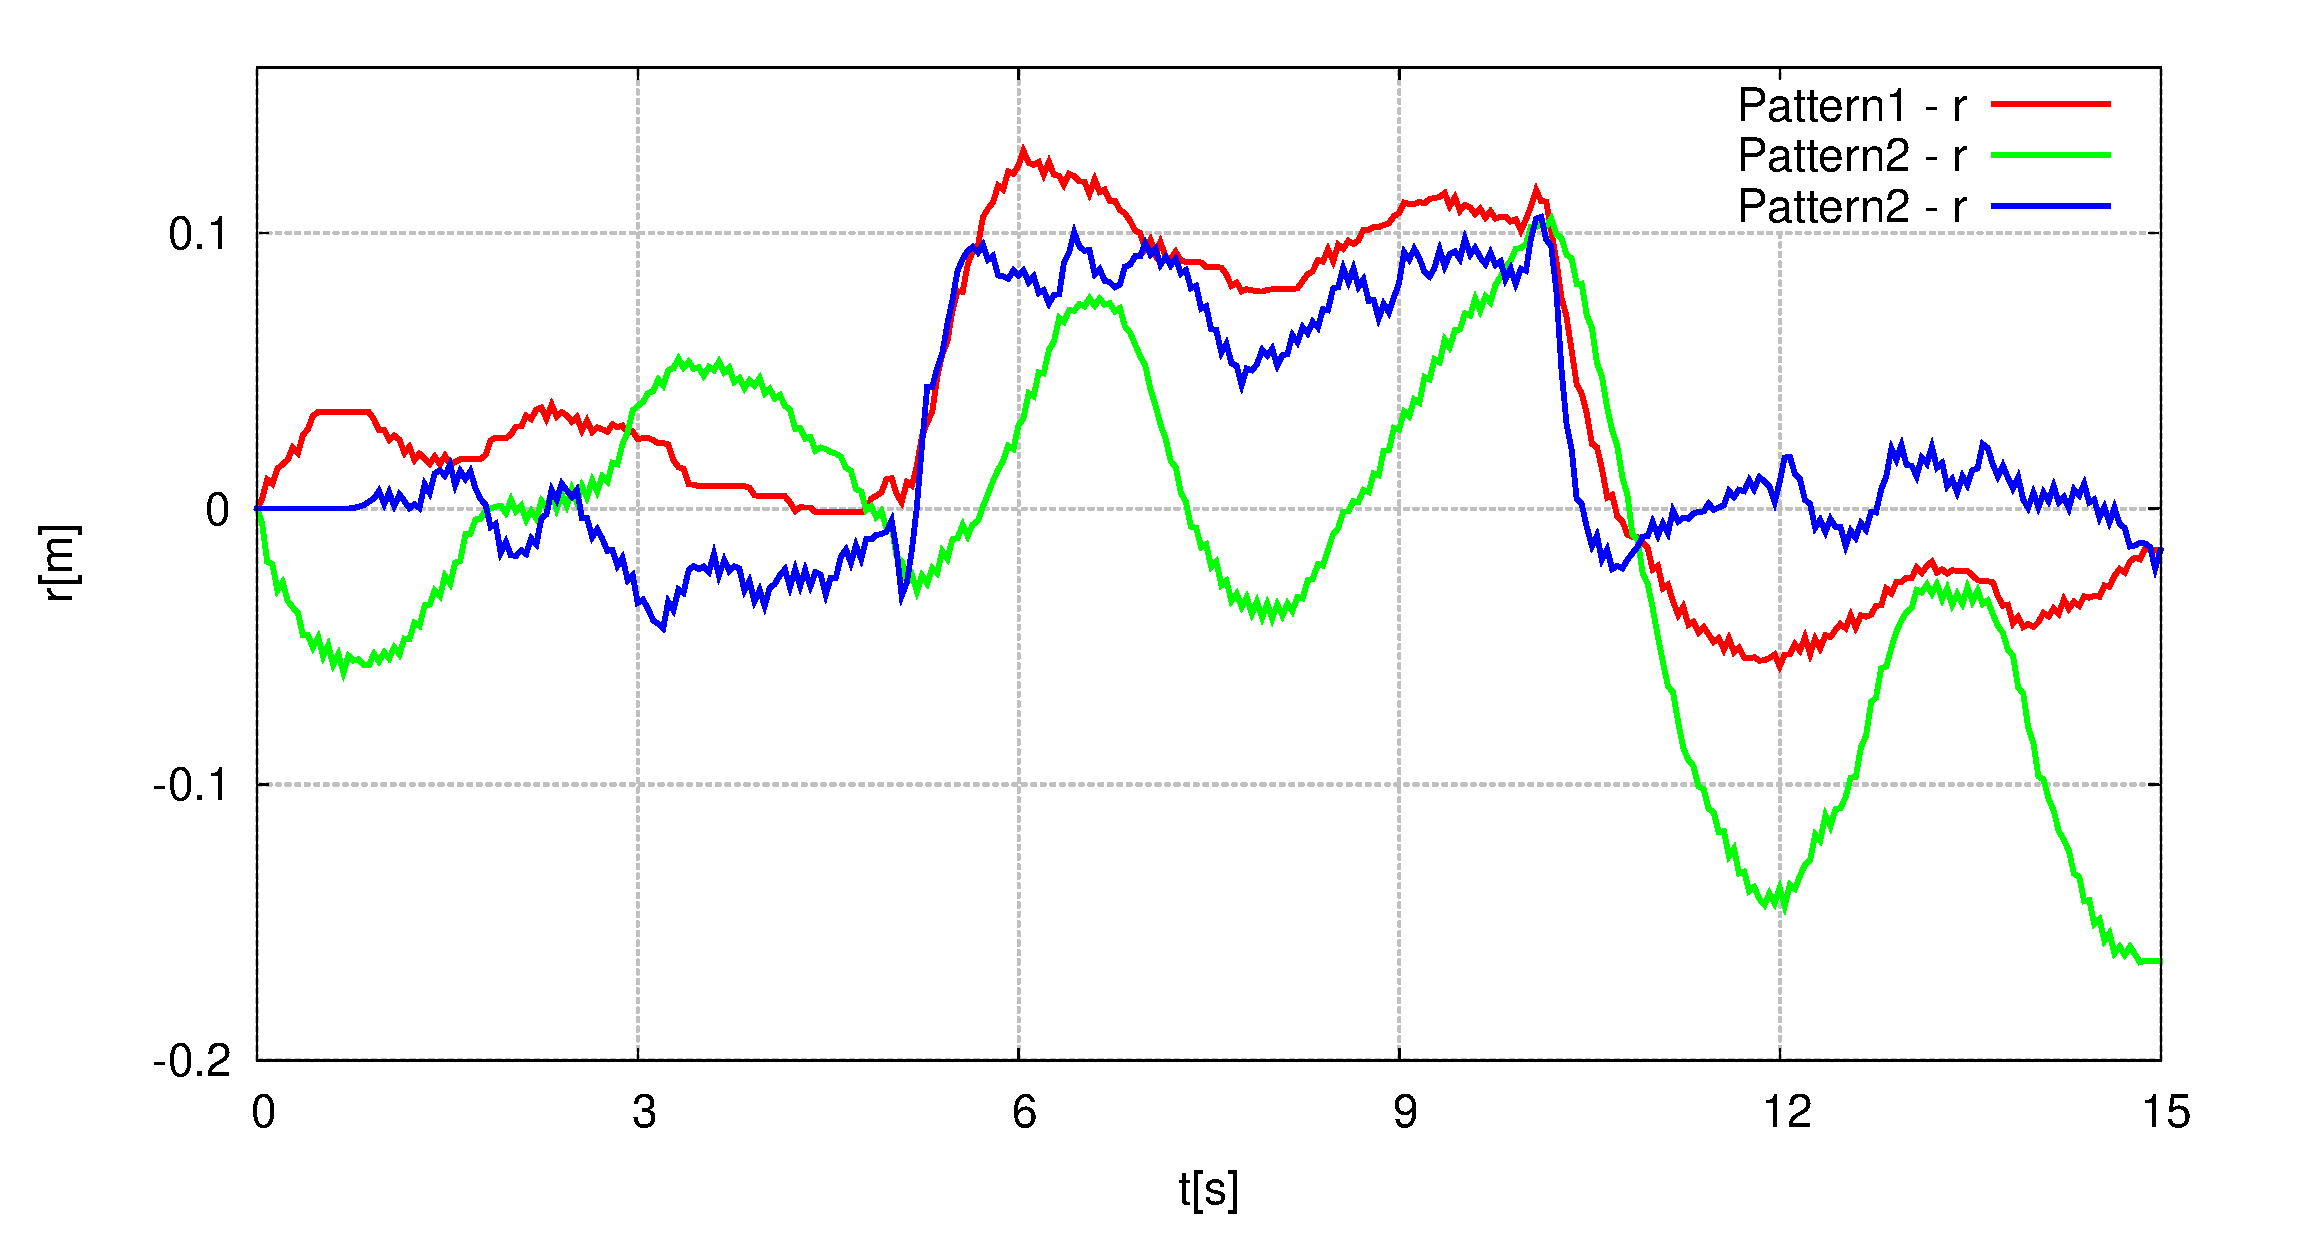
\includegraphics[width=0.49\linewidth]{gazo/Compare_Q_R.eps}
		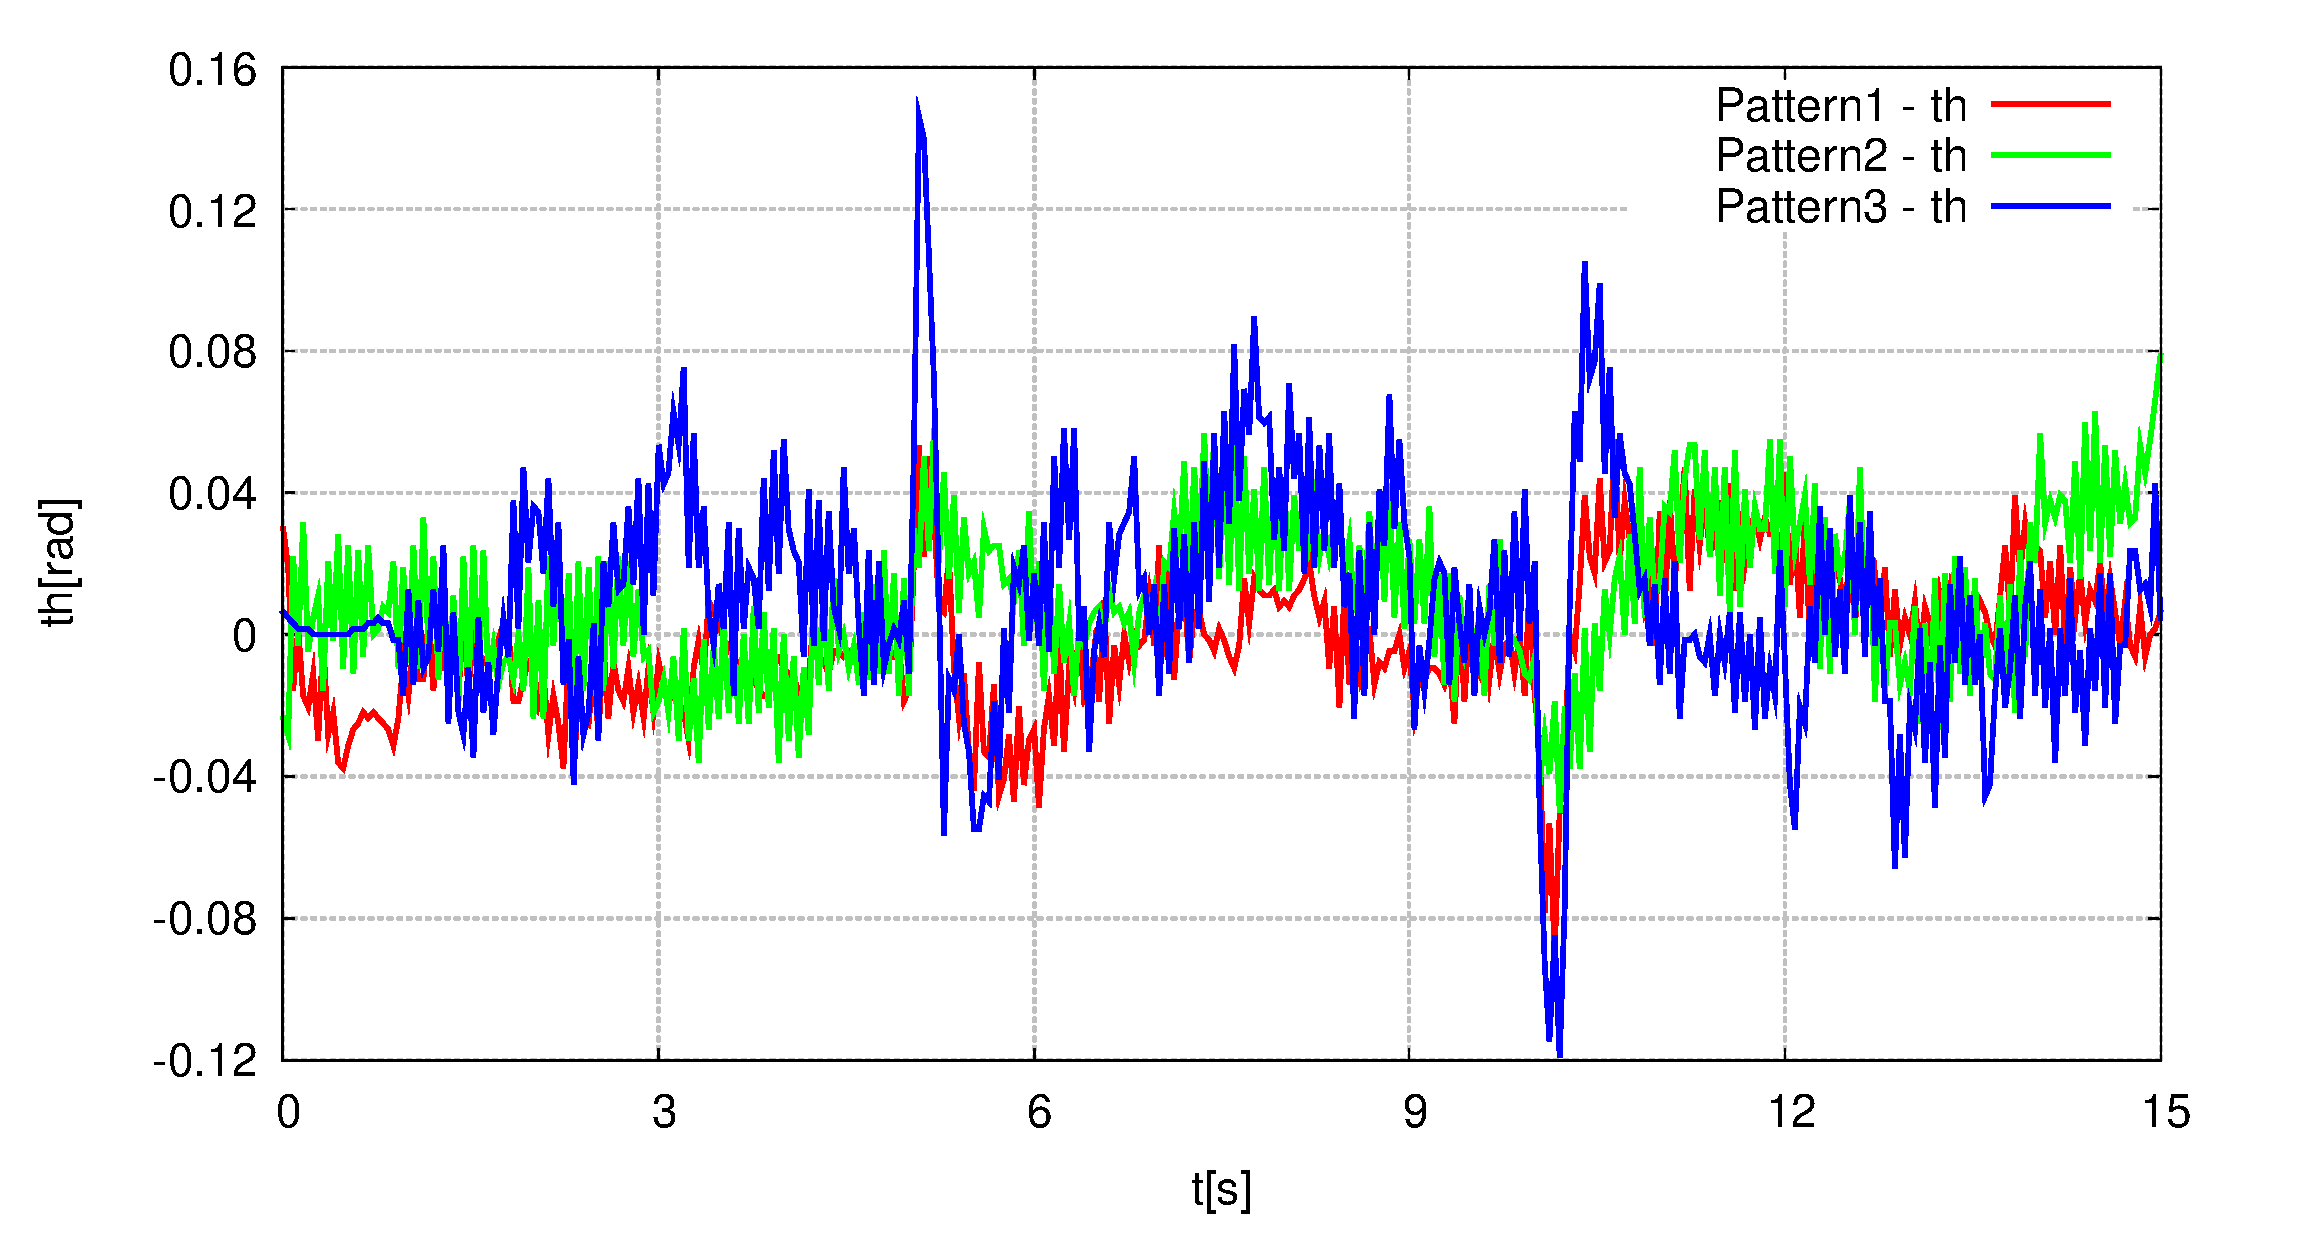
\includegraphics[width=0.49\linewidth]{gazo/Compare_Q_TH.eps}
		\caption{重み行列の違いによる実験結果の比較}
		\label{image:comp_Q}
	\end{figure}
	図中のPatternは以下の表に対応するパラメータである。
	\begin{table}[H]
		\begin{center}
			\caption{パターンとパラメータの対応表}
			\medskip
			
			\begin{tabular}{|c|c|c|c|}\hline
				パターン & 重み行列$Q$ & オブザーバの極$P$ & サンプリング周期$\Delta[\rm{s}]$ \\ \hline\hline
				Pattern1 & $Q_1$:$\rm{diag}(1E5,1E5,1,1)$ & $P_1$:$((-30,0),(-30,0))^{'}$ & $\Delta_1$:0.005 \\ \hline
				Pattern2 & $Q_1$:$\rm{diag}(1E5,1E6,1,1)$ & $P_1$:$((-30,0),(-30,0))^{'}$ & $\Delta_1$:0.005 \\ \hline
				Pattern3 & $Q_1$:$\rm{diag}(1E6,1E5,1,1)$ & $P_1$:$((-30,0),(-30,0))^{'}$ & $\Delta_1$:0.005 \\ \hline
			\end{tabular}
		\end{center}
		\label{table:huriage_control}
	\end{table}
	図\ref{image:comp_Q}の左図を見えると、ノイズがひどいがPattern1、Pattern2は目標値の変更に追従
	できているが、Pattern3は目標値の変更に追従できていない。また、Pattern1とPattern2では大きな違いは確認できないが、
	若干Pattern1のほうが応答が目標値に追従できている。
	右図からは、Pattern3が目標値変更の時間(5秒と10秒)において角度が大きく出ており、一番応答が悪いといえる。
	このことからシミュレーションで行った考察と概ね一致しているといえる。しかし、シミュレーションのときには
	現れなかった目標値変化への追従性の違いが現れた。また、シミュレーションでは応答を良くしたい状態に対応する成分を
	大きくすればよいと考察したが、実験結果からは、重み行列に偏りをつけるより、良くしたい状態に対応する成分をバランスよく
	大きくしたほうが応答がよくなったといえる。
	\par
	\subsection{オブザーバの極の違いによる実験結果の比較}
	次にオブザーバの極の違いによる実験結果の比較を見てみる。
	\begin{figure}[H]
		\centering
		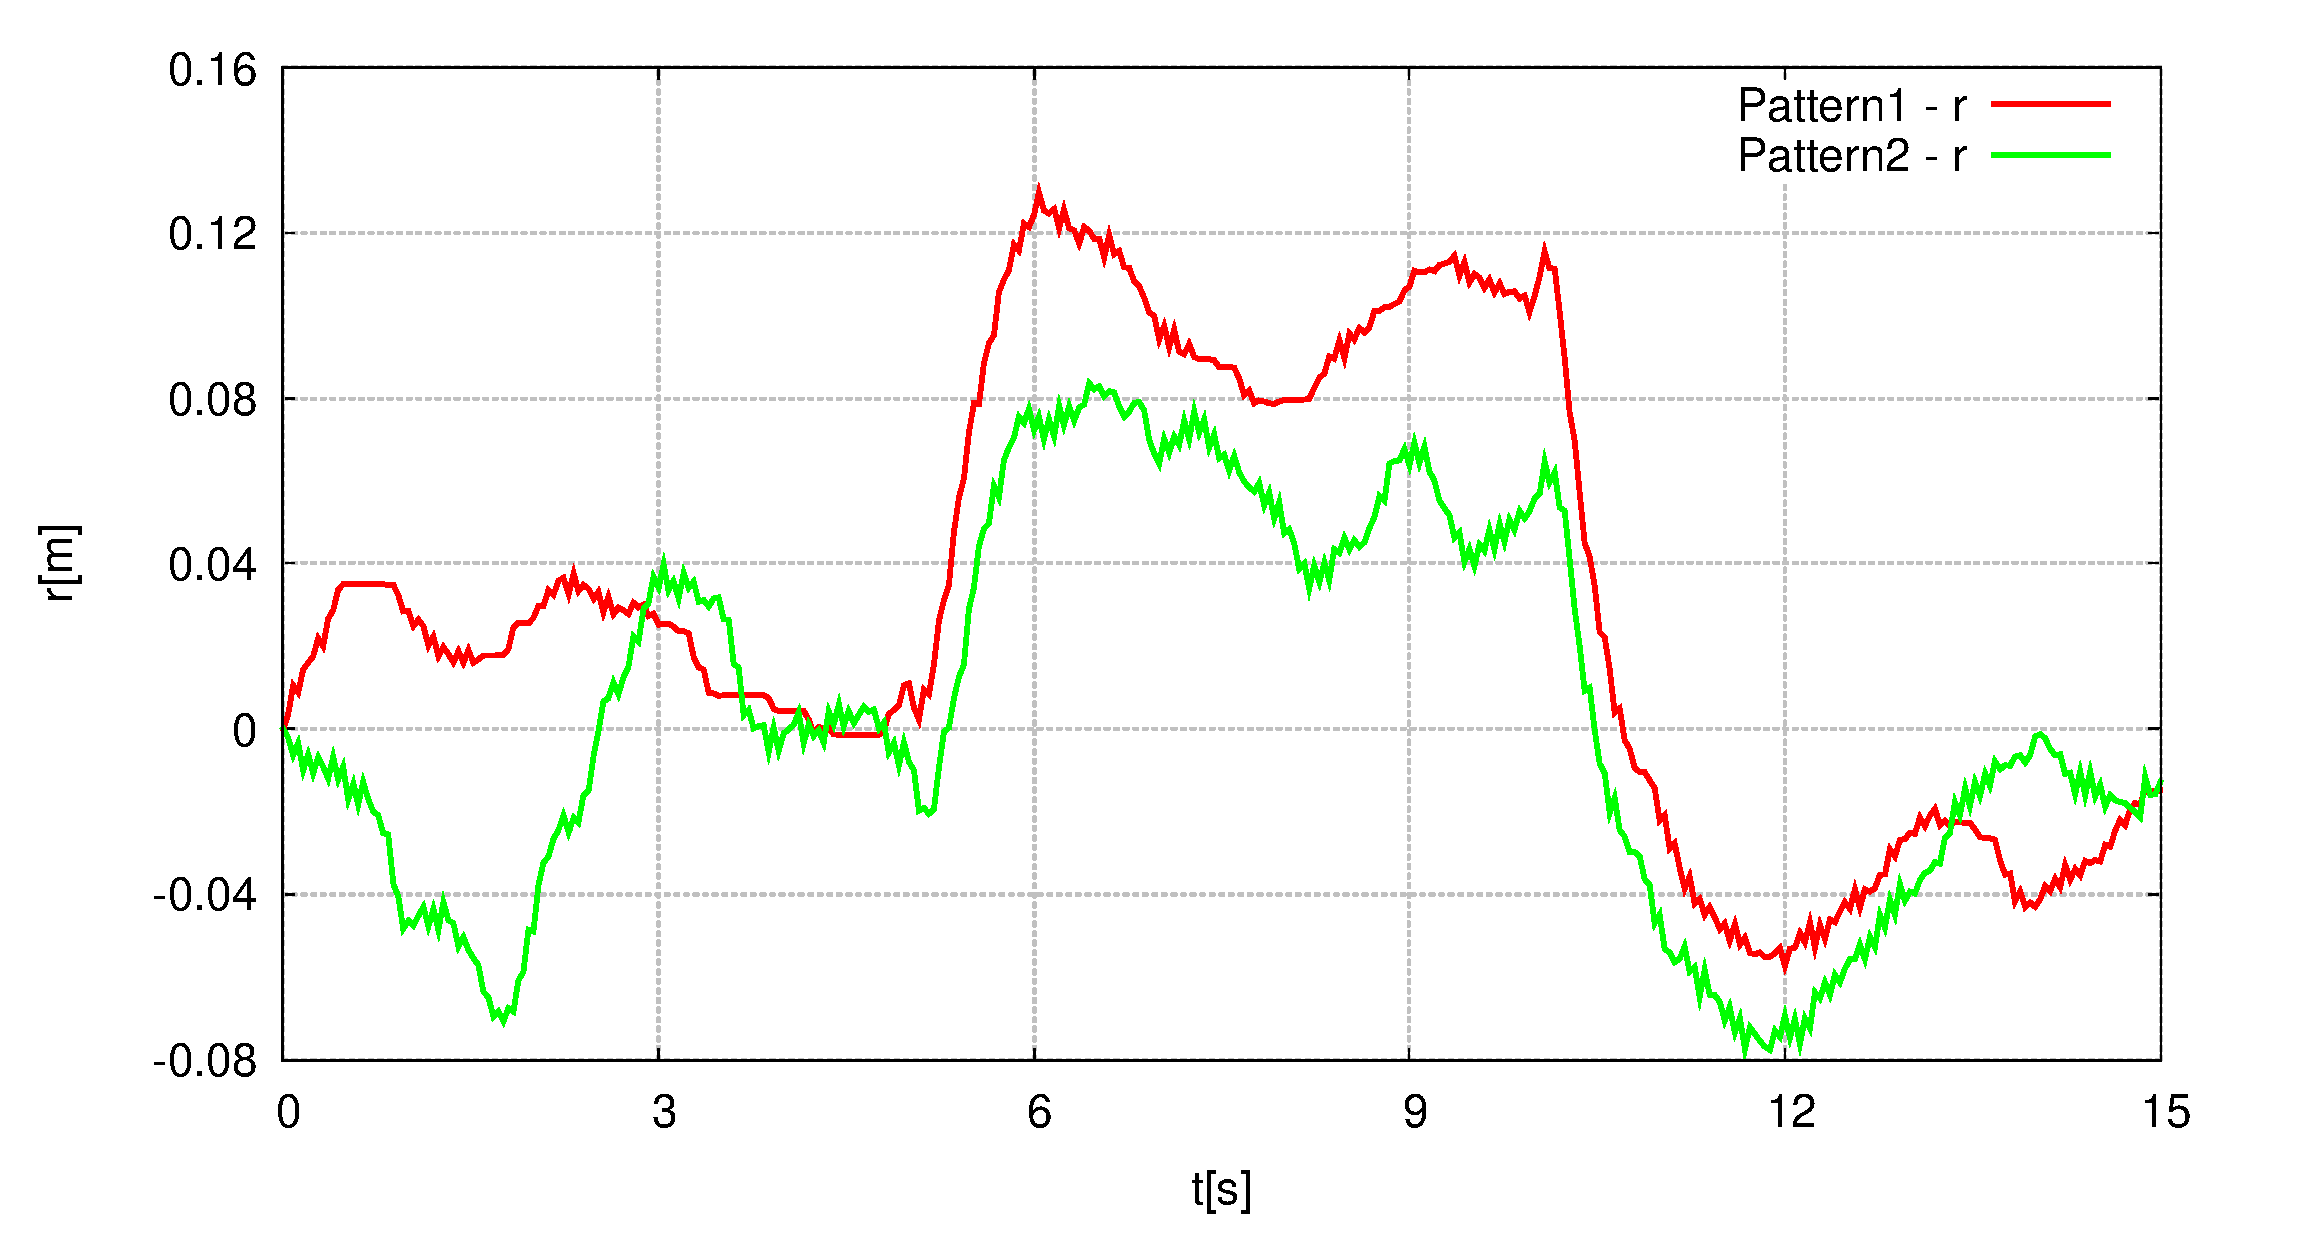
\includegraphics[width=0.49\linewidth]{gazo/Compare_obs_R.eps}
		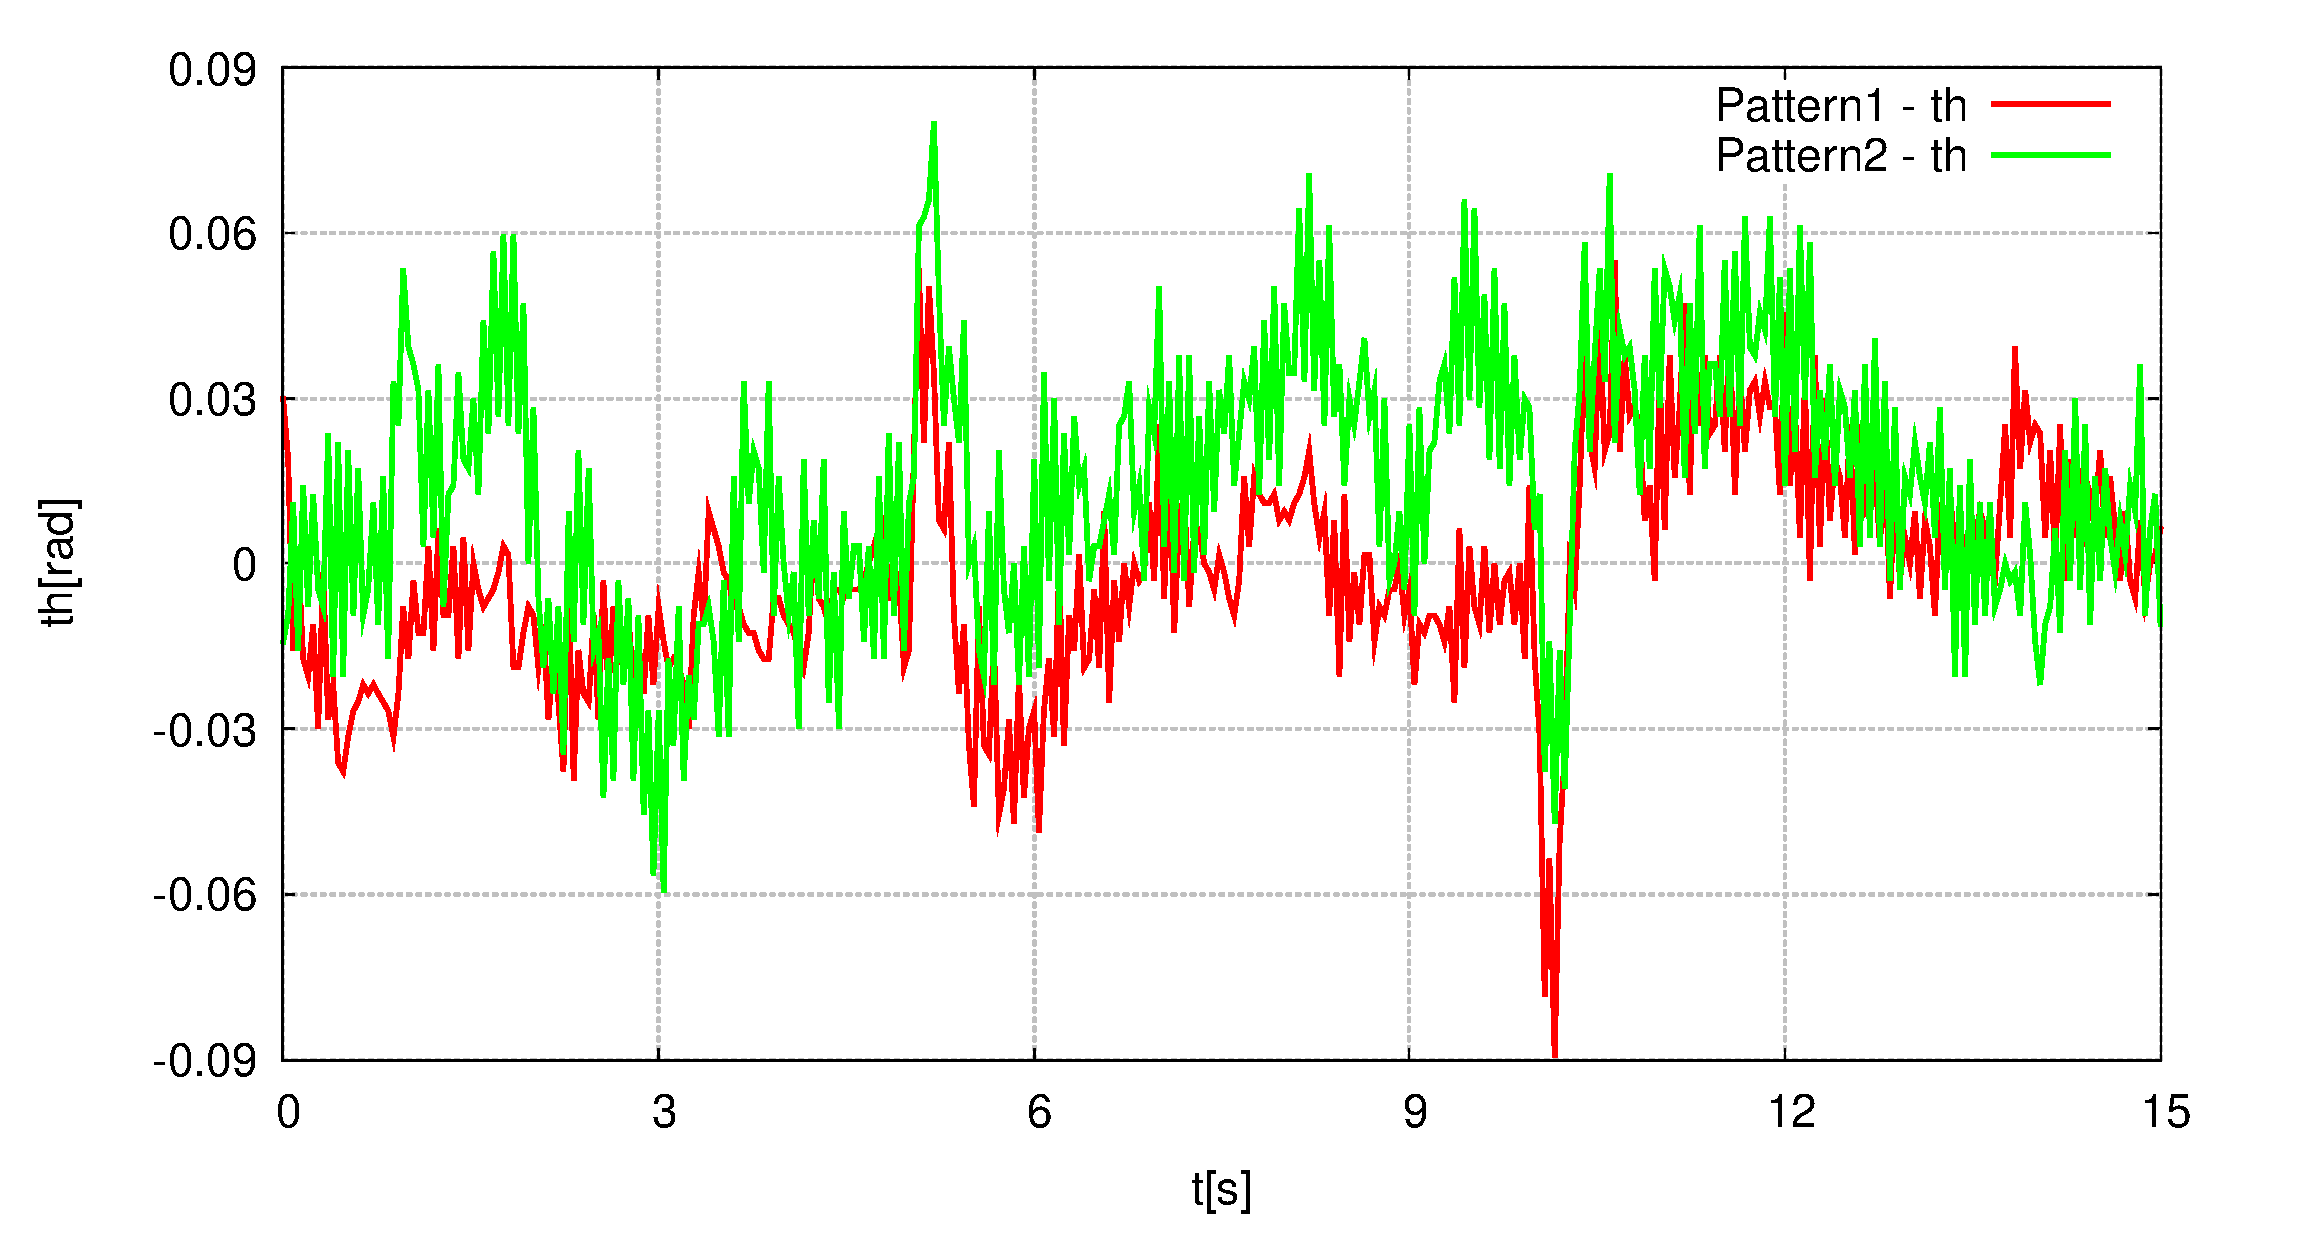
\includegraphics[width=0.49\linewidth]{gazo/Compare_obs_TH.eps}
		\caption{オブザーバの極の違いによる実験結果の比較}
		\label{image:comp_obs}
	\end{figure}
	図中のPatternは以下の表に対応するパラメータである。
	\begin{table}[H]
		\begin{center}
			\caption{パターンとパラメータの対応表}
			\medskip
			
			\begin{tabular}{|c|c|c|c|}\hline
				パターン & 重み行列$Q$ & オブザーバの極$P$ & サンプリング周期$\Delta[\rm{s}]$ \\ \hline\hline
				Pattern1 & $Q_1$:$\rm{diag}(1E5,1E5,1,1)$ & $P_1$:$((-30,0),(-30,0))^{'}$ & $\Delta_1$:0.005 \\ \hline
				Pattern2 & $Q_1$:$\rm{diag}(1E5,1E6,1,1)$ & $P_1$:$((-60,0),(-60,0))^{'}$ & $\Delta_1$:0.005 \\ \hline
			\end{tabular}
		\end{center}
		\label{table:huriage_control}
	\end{table}
	図\ref{image:comp_obs}の左図より、台車の位置についてはPattern2よりもPattern1の方が目標値変化に追従できているといえる。
	つまり、オブザーバの極が虚軸に近い方が目標値変化へ追従できるといえる。
	シミュレーションのときには大きな違いが出なかったが、実験においては目標値変化への追従性という形で違いが出てきている。
	右図より、振子の角度については、Pattern1とPattern2では大きな違いは確認できないといえる。
	\newpage
	\subsection{サンプリング周期の違いによる実験結果の比較}
	次にサンプリング周期の違いによる実験結果の比較を見てみる。
	\begin{figure}[H]
		\centering
		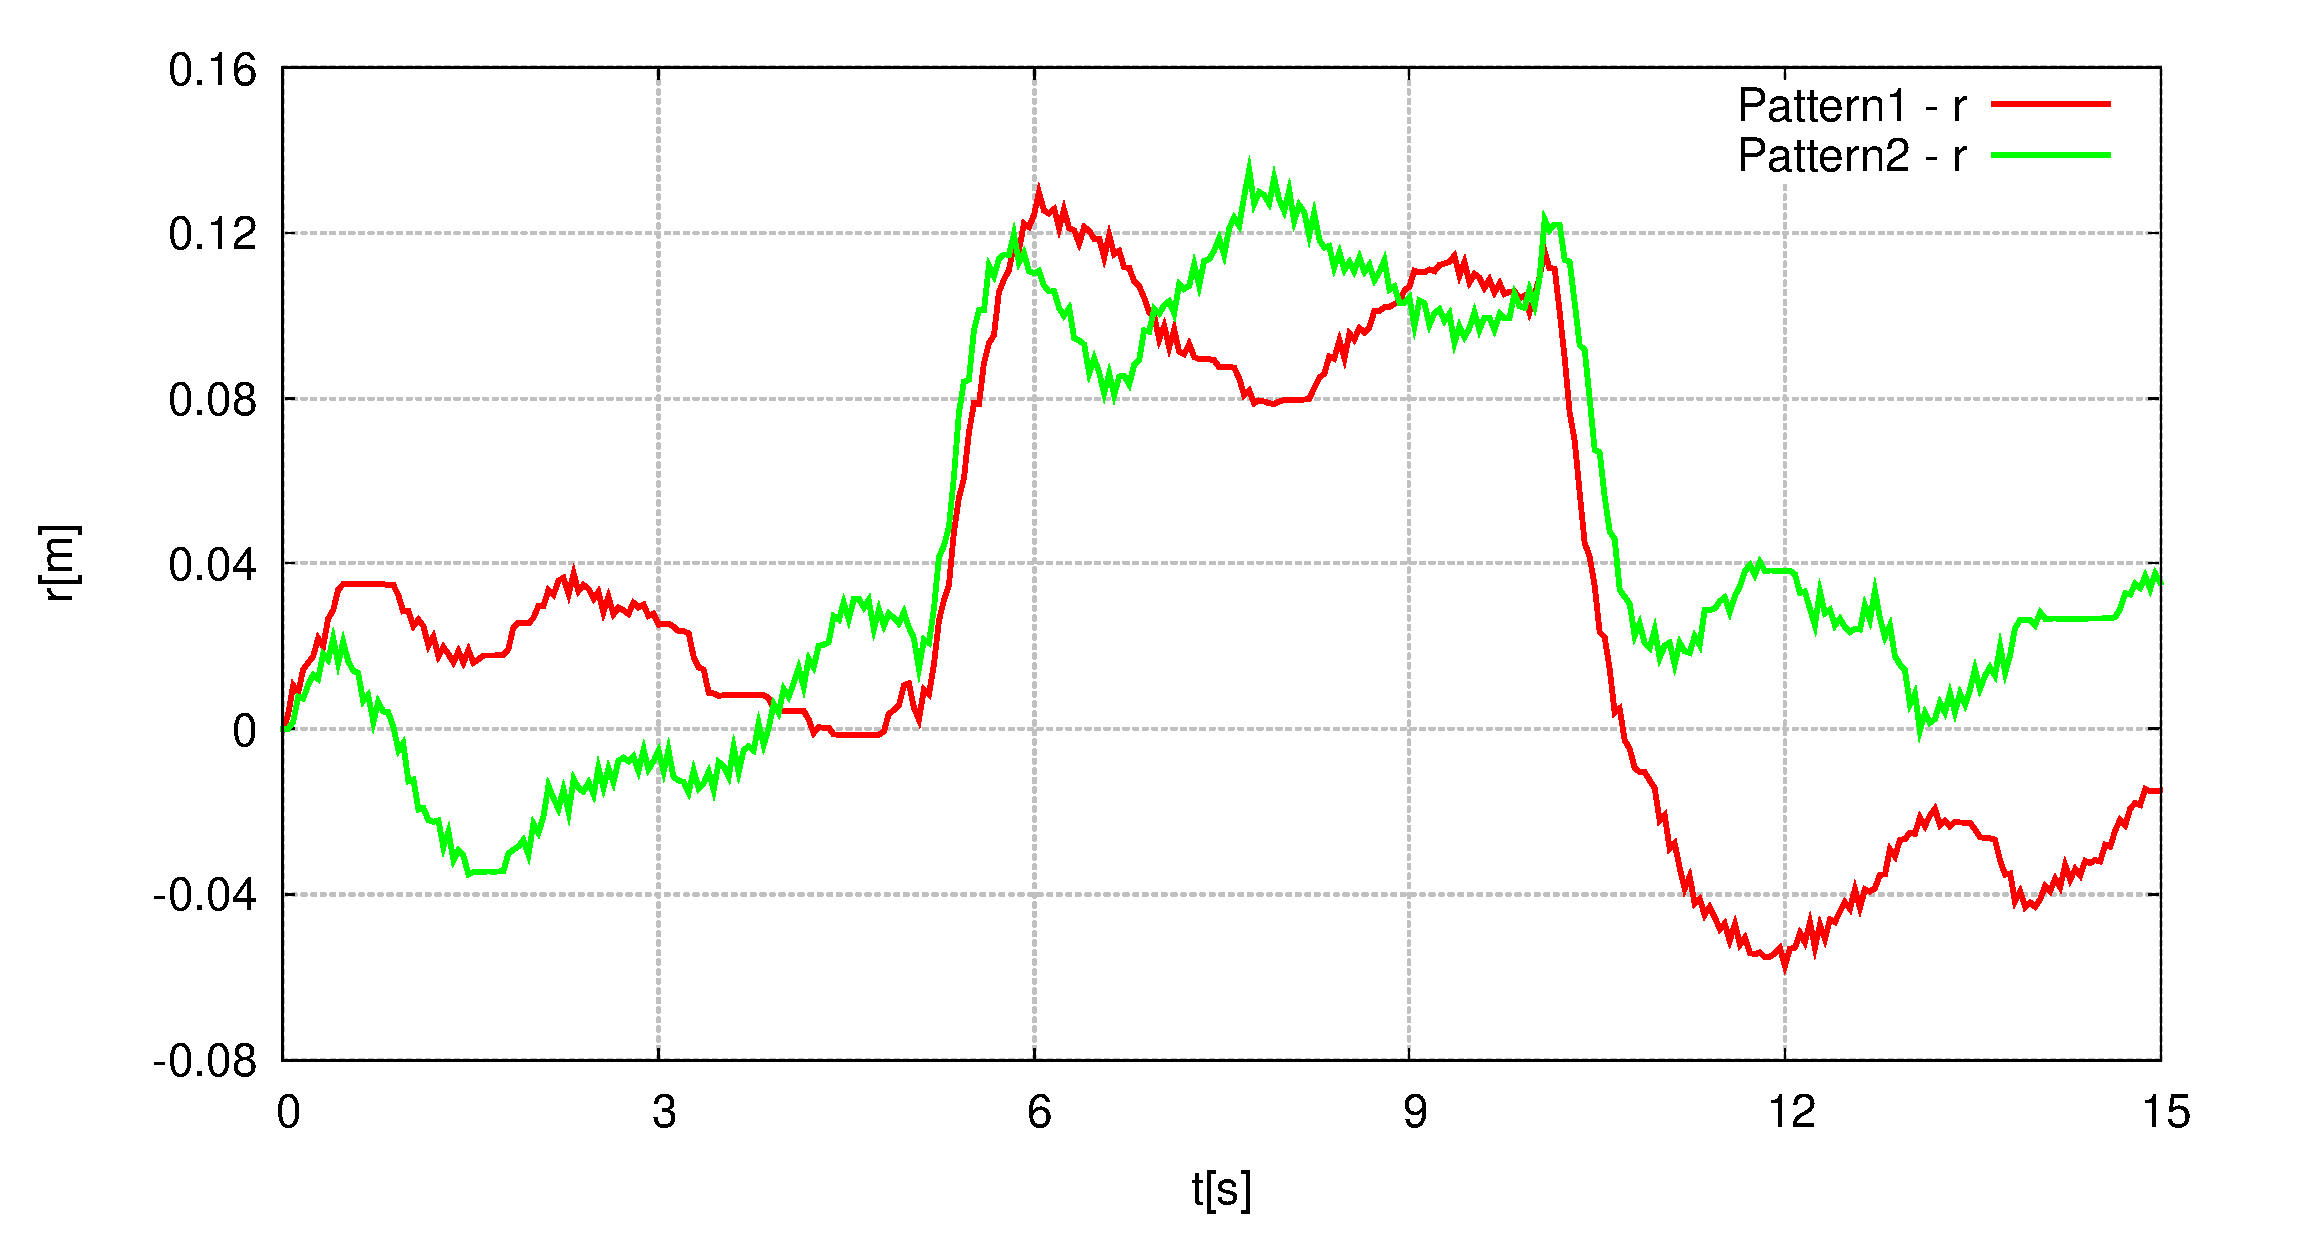
\includegraphics[width=0.49\linewidth]{gazo/Compare_dt_R.eps}
		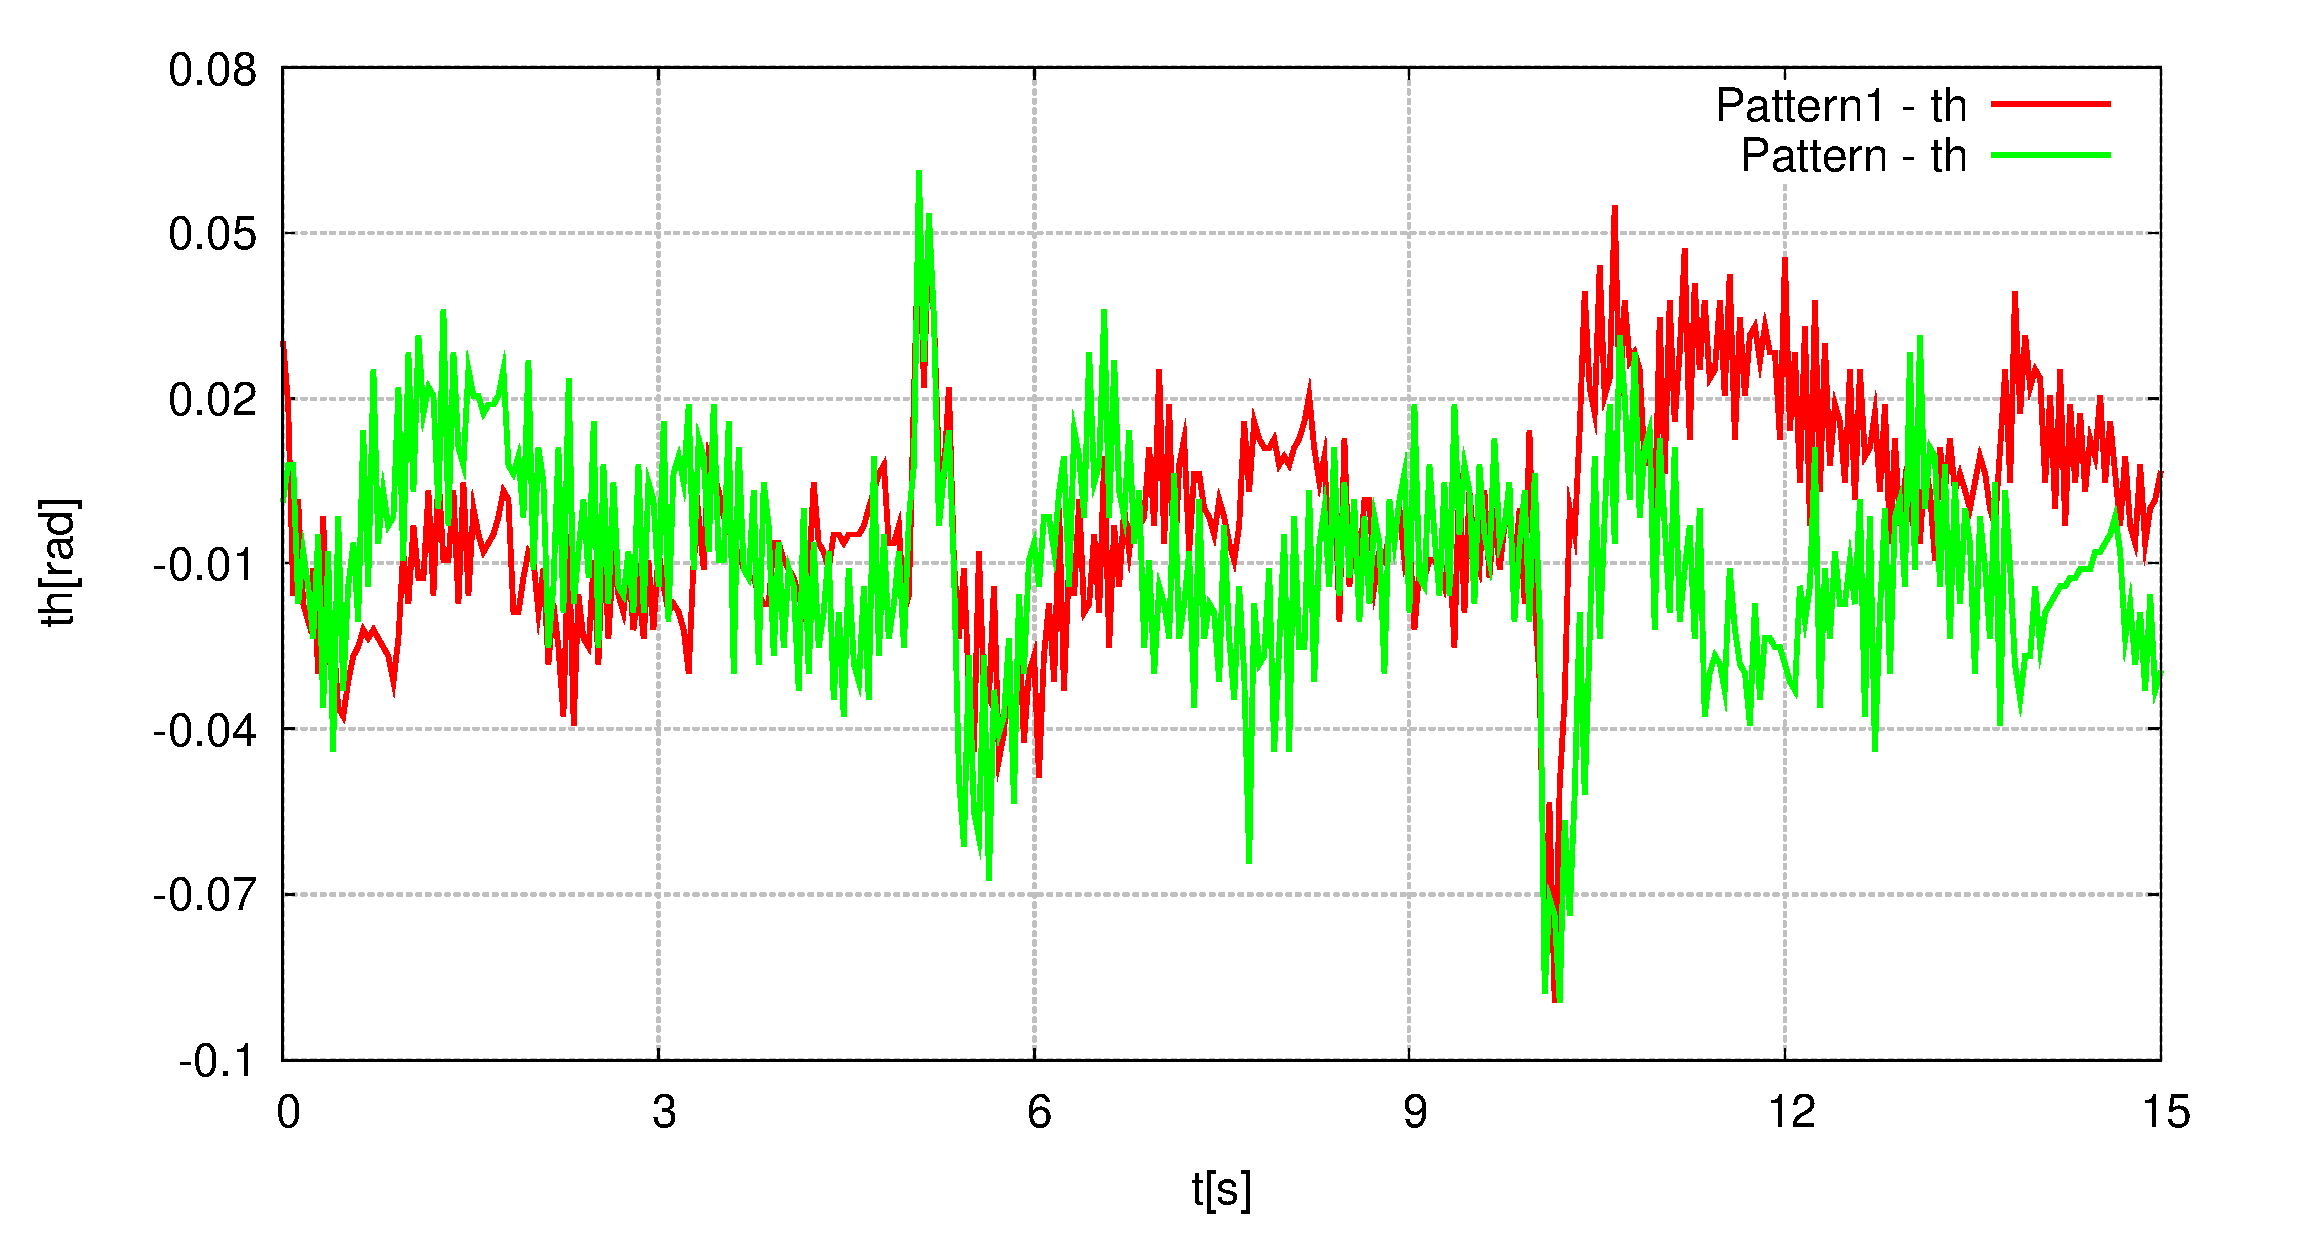
\includegraphics[width=0.49\linewidth]{gazo/Compare_dt_TH.eps}
		\caption{サンプリング周期の違いによる実験結果の比較}
		\label{image:comp_dt}
	\end{figure}
	図中のPatternは以下の表に対応するパラメータである。
	\begin{table}[H]
		\begin{center}
			\caption{パターンとパラメータの対応表}
			\medskip
			
			\begin{tabular}{|c|c|c|c|}\hline
				パターン & 重み行列$Q$ & オブザーバの極$P$ & サンプリング周期$\Delta[\rm{s}]$ \\ \hline\hline
				Pattern1 & $Q_1$:$\rm{diag}(1E5,1E5,1,1)$ & $P_1$:$((-30,0),(-30,0))^{'}$ & $\Delta_1$:0.005 \\ \hline
				Pattern2 & $Q_1$:$\rm{diag}(1E5,1E6,1,1)$ & $P_1$:$((-30,0),(-30,0))^{'}$ & $\Delta_1$:0.010 \\ \hline
			\end{tabular}
		\end{center}
		\label{table:huriage_control}
	\end{table}
	図\ref{image:comp_dt}の左図より、台車の位置については2パターンとも大きな違いはないといえる。右図より、振子の角度についても2パターンとも
	大きな違いはないといえる。このことから概ねシミュレーションと同じ結果を得ることができたといえる。
	\newpage
	\subsection{シミュレーション結果と実験結果の比較}
	以下に実験結果とシミュレーション結果との比較を行った図を示す。
	また、図の数が多いので図のキャプションとその図における各パラメータの対応表を示す。
	\begin{table}[H]
		\begin{center}
			\caption{図に対応するパラメータの組}
			\begin{tabular}{|c|c|c|c|}\hline
				図のキャプション & 重み行列$Q$ & オブザーバの極$P$ & サンプリング周期$\Delta[\rm{s}]$ \\ \hline\hline
				比較結果その1 & $Q_1$:$\rm{diag}(1E5,1E5,1,1)$ & $P_1$:$((-30,0),(-30,0))^{'}$ & $\Delta_1$:0.005 \\ \hline
				比較結果その2 & $Q_1$:$\rm{diag}(1E5,1E6,1,1)$ & $P_1$:$((-30,0),(-30,0))^{'}$ & $\Delta_1$:0.005 \\ \hline
				比較結果その3 & $Q_1$:$\rm{diag}(1E6,1E5,1,1)$ & $P_1$:$((-30,0),(-30,0))^{'}$ & $\Delta_1$:0.005 \\ \hline
				比較結果その4 & $Q_1$:$\rm{diag}(1E5,1E5,1,1)$ & $P_1$:$((-60,0),(-30,0))^{'}$ & $\Delta_1$:0.005 \\ \hline
				比較結果その5 & $Q_1$:$\rm{diag}(1E5,1E6,1,1)$ & $P_1$:$((-60,0),(-30,0))^{'}$ & $\Delta_1$:0.005 \\ \hline
				比較結果その6 & $Q_1$:$\rm{diag}(1E6,1E5,1,1)$ & $P_1$:$((-60,0),(-30,0))^{'}$ & $\Delta_1$:0.005 \\ \hline
				比較結果その7 & $Q_1$:$\rm{diag}(1E5,1E5,1,1)$ & $P_1$:$((-30,0),(-30,0))^{'}$ & $\Delta_1$:0.010 \\ \hline
				比較結果その8 & $Q_1$:$\rm{diag}(1E5,1E6,1,1)$ & $P_1$:$((-30,0),(-30,0))^{'}$ & $\Delta_1$:0.010 \\ \hline
				比較結果その9 & $Q_1$:$\rm{diag}(1E6,1E5,1,1)$ & $P_1$:$((-30,0),(-30,0))^{'}$ & $\Delta_1$:0.010 \\ \hline
				比較結果その10 & $Q_1$:$\rm{diag}(1E5,1E5,1,1)$ & $P_1$:$((-60,0),(-30,0))^{'}$ & $\Delta_1$:0.010 \\ \hline
				比較結果その11 & $Q_1$:$\rm{diag}(1E5,1E6,1,1)$ & $P_1$:$((-60,0),(-30,0))^{'}$ & $\Delta_1$:0.010 \\ \hline
				比較結果その12 & $Q_1$:$\rm{diag}(1E6,1E5,1,1)$ & $P_1$:$((-60,0),(-30,0))^{'}$ & $\Delta_1$:0.010 \\ \hline
			\end{tabular}
		\end{center}
		\label{table:huriage_control}
	\end{table}
	
	\begin{figure}[H]
		\centering
		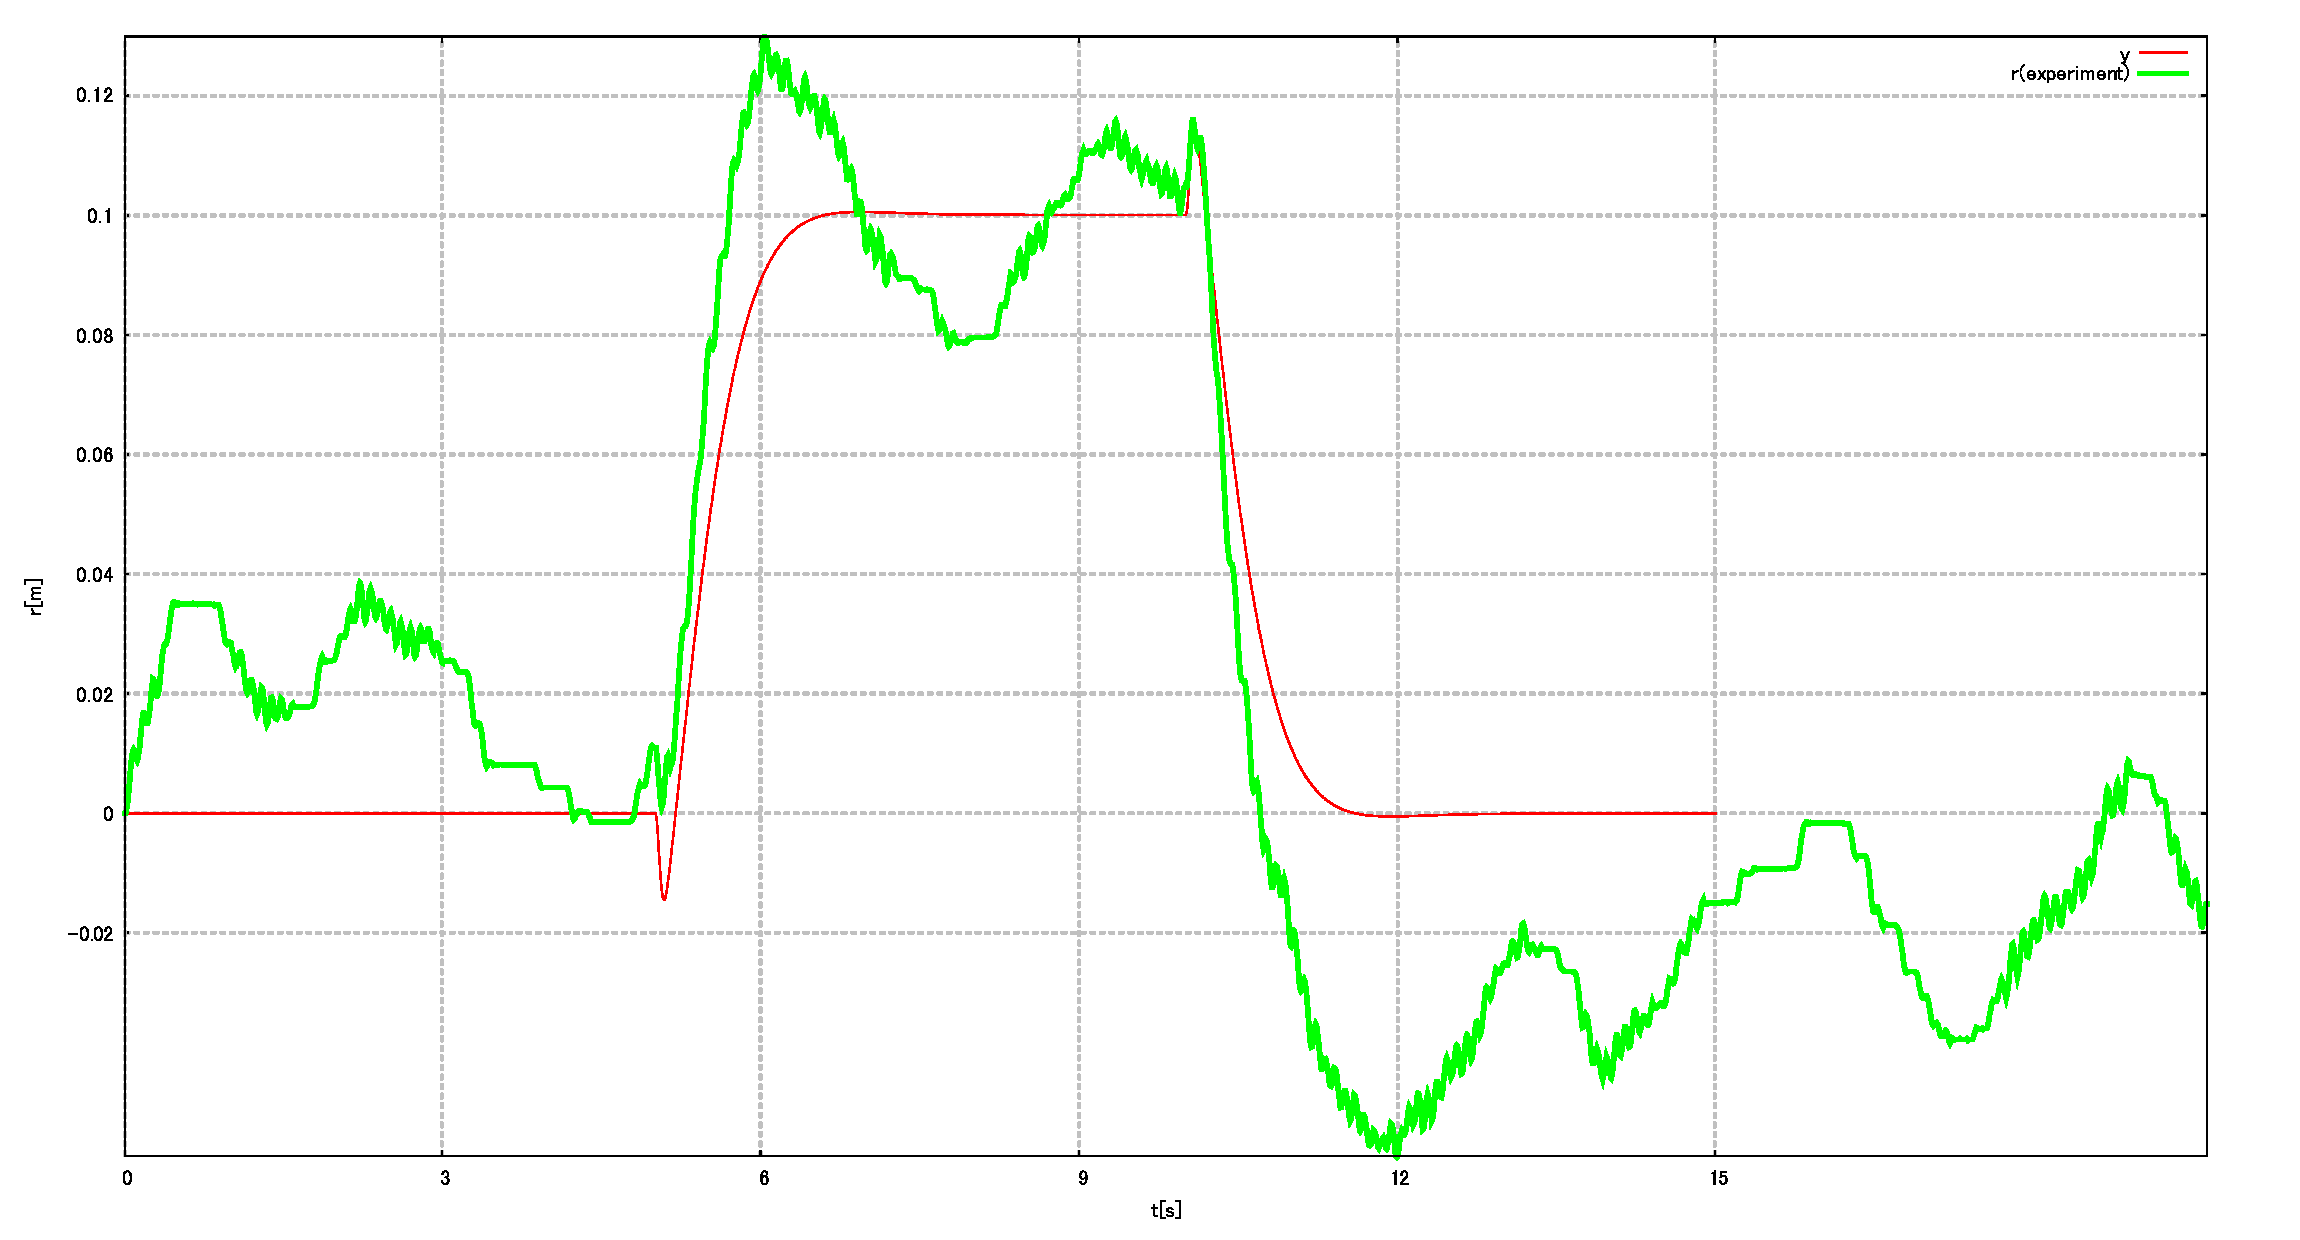
\includegraphics[width=0.49\linewidth]{gazo/experiment_Q55obs30dt05R.eps}
		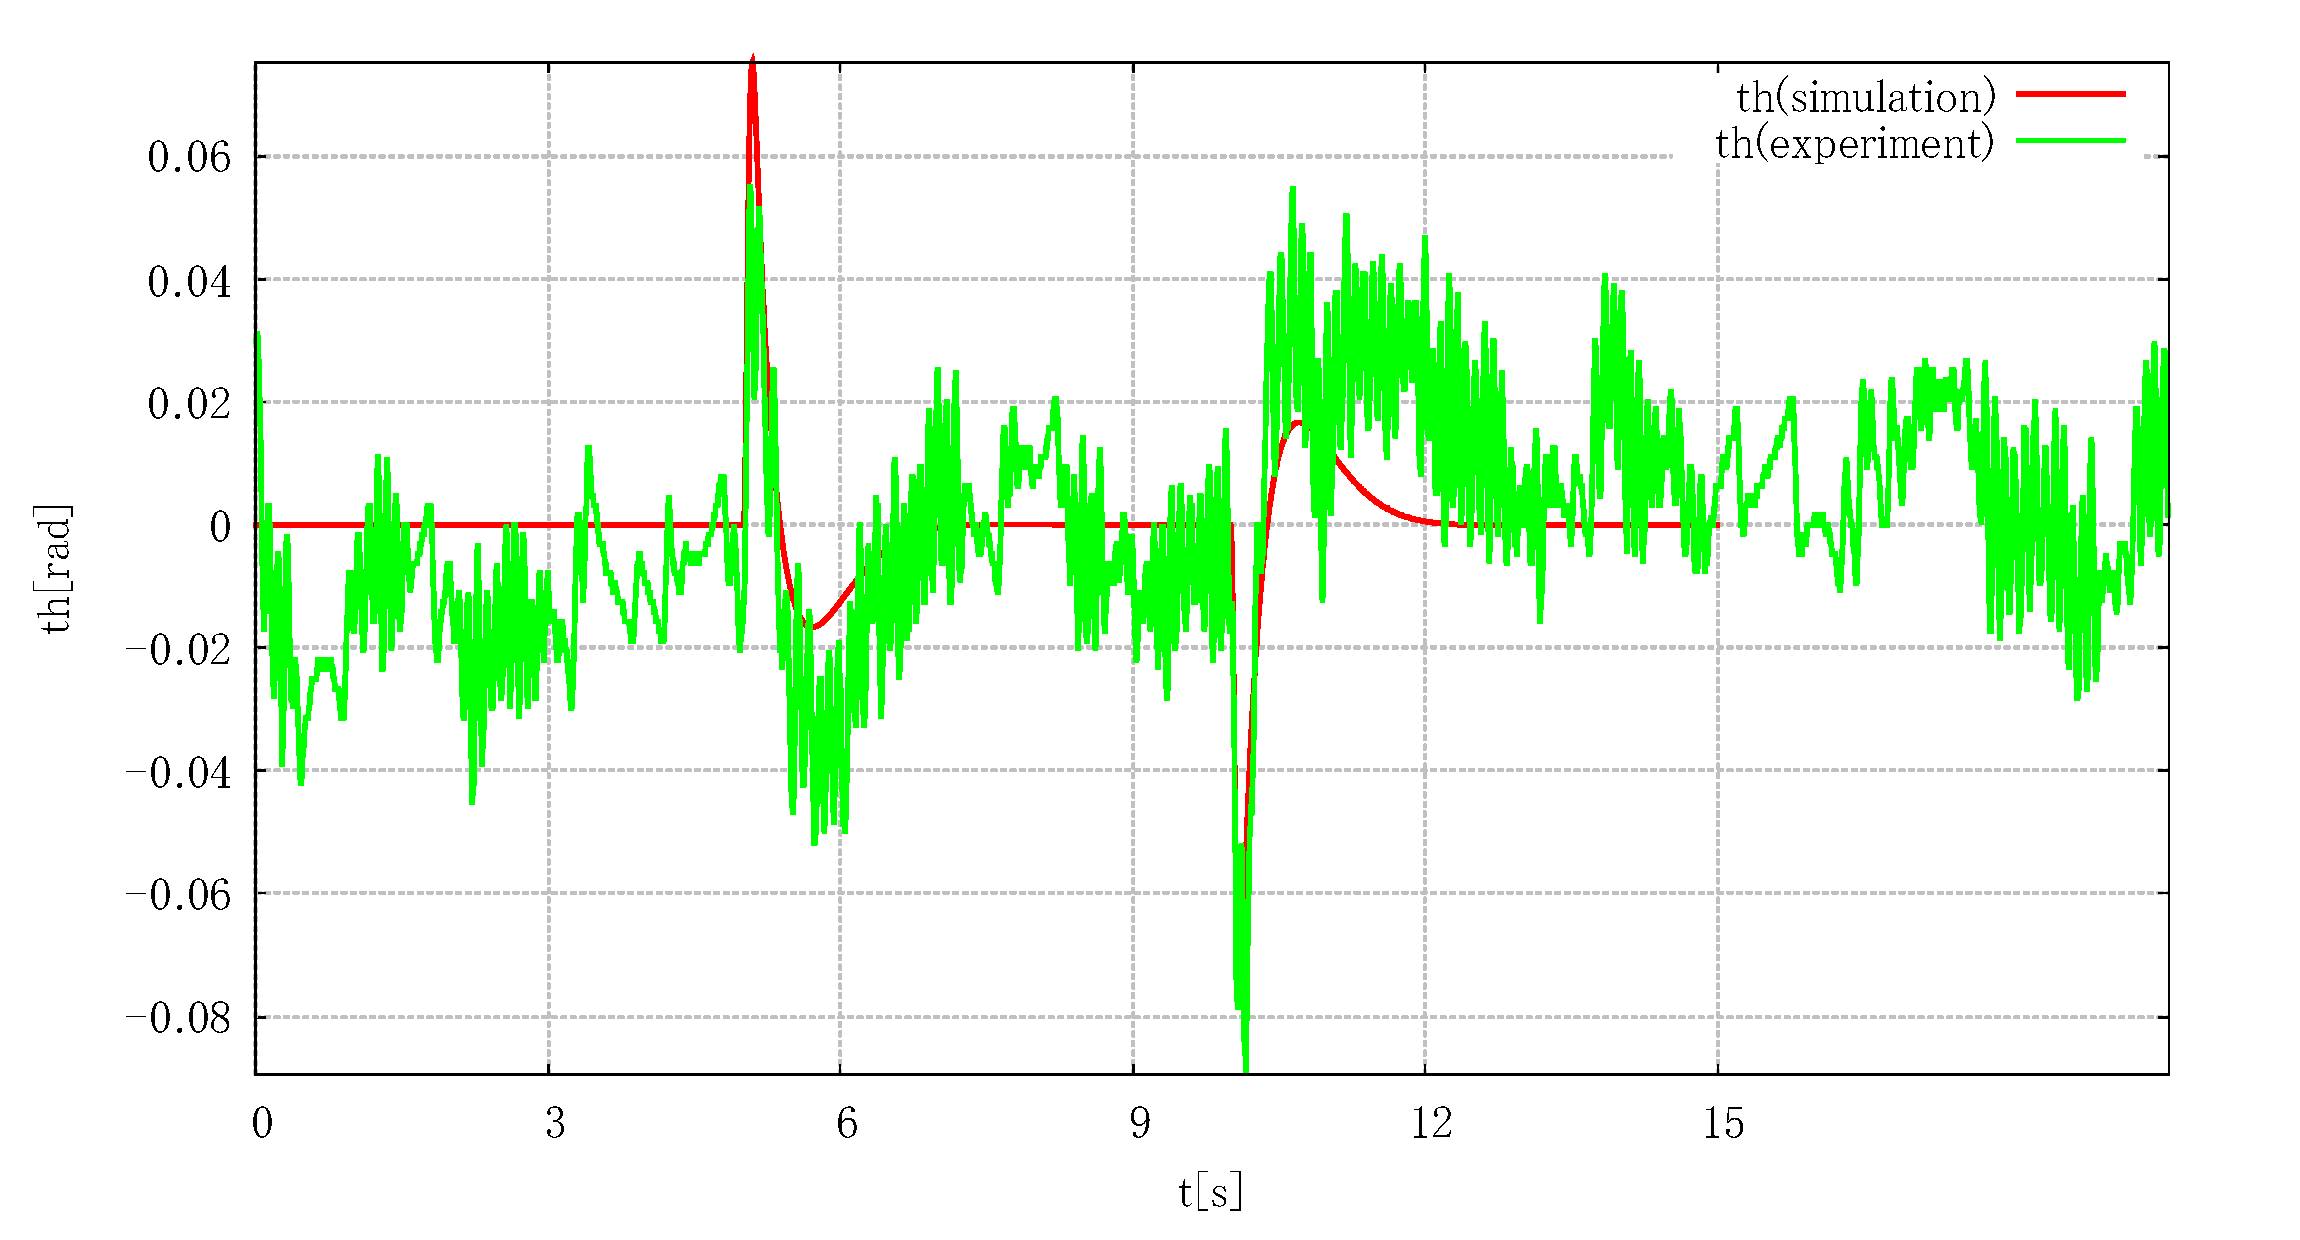
\includegraphics[width=0.49\linewidth]{gazo/experiment_Q55obs30dt05TH.eps}
		\caption{比較結果その1(左図がr,右図が$\theta$)}
		\label{image:sono1}
	\end{figure}
	\begin{figure}[H]
		\centering
		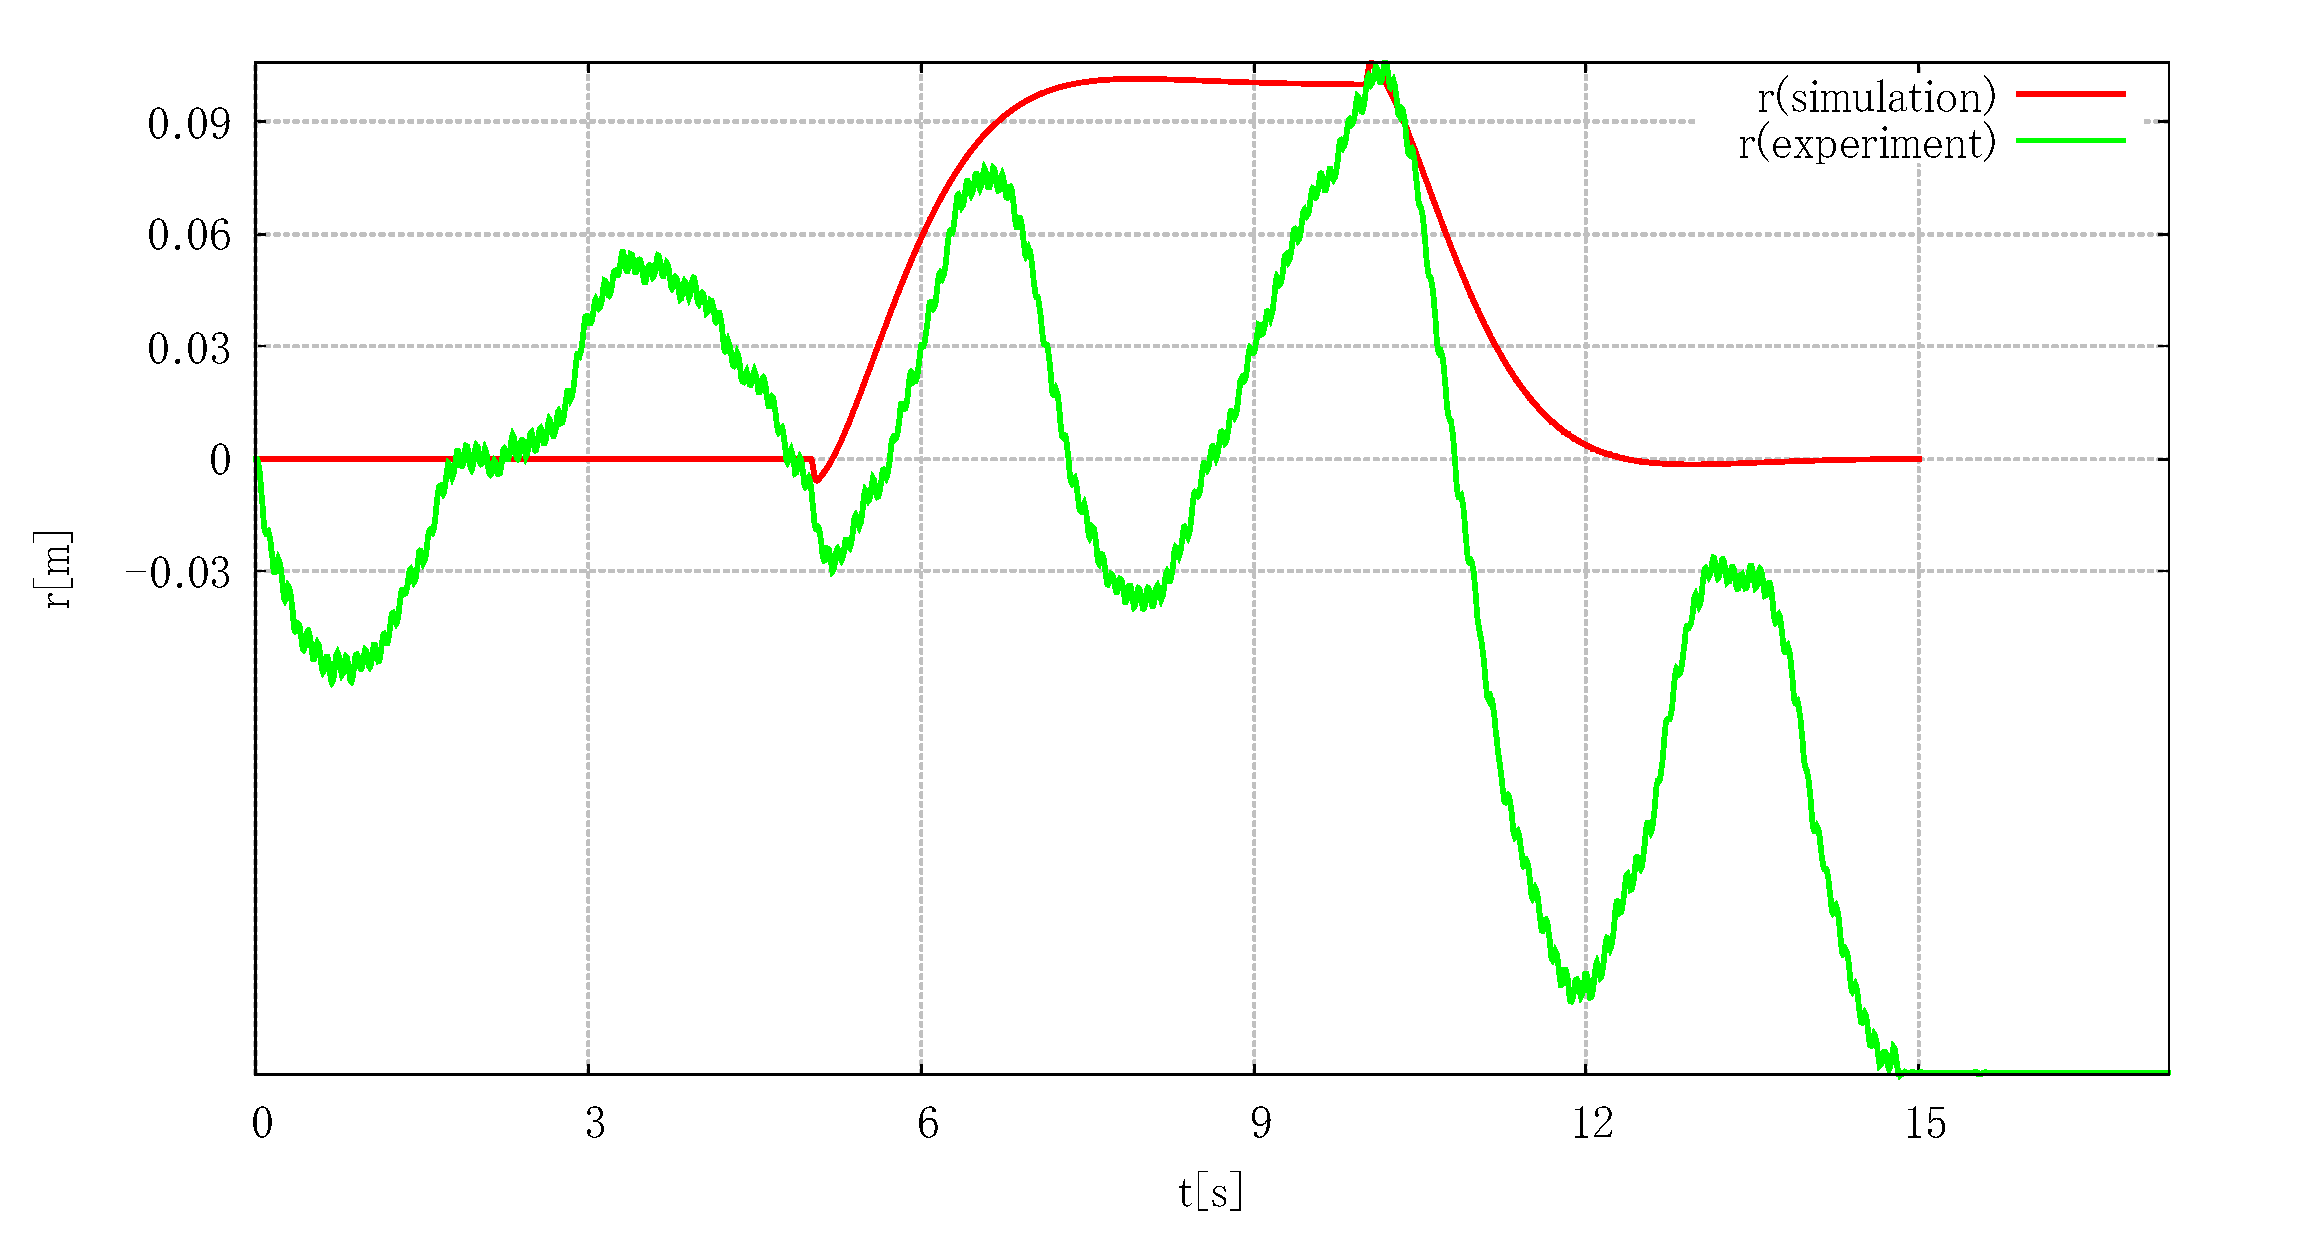
\includegraphics[width=0.49\linewidth]{gazo/experiment_Q56obs30dt05R.eps}
		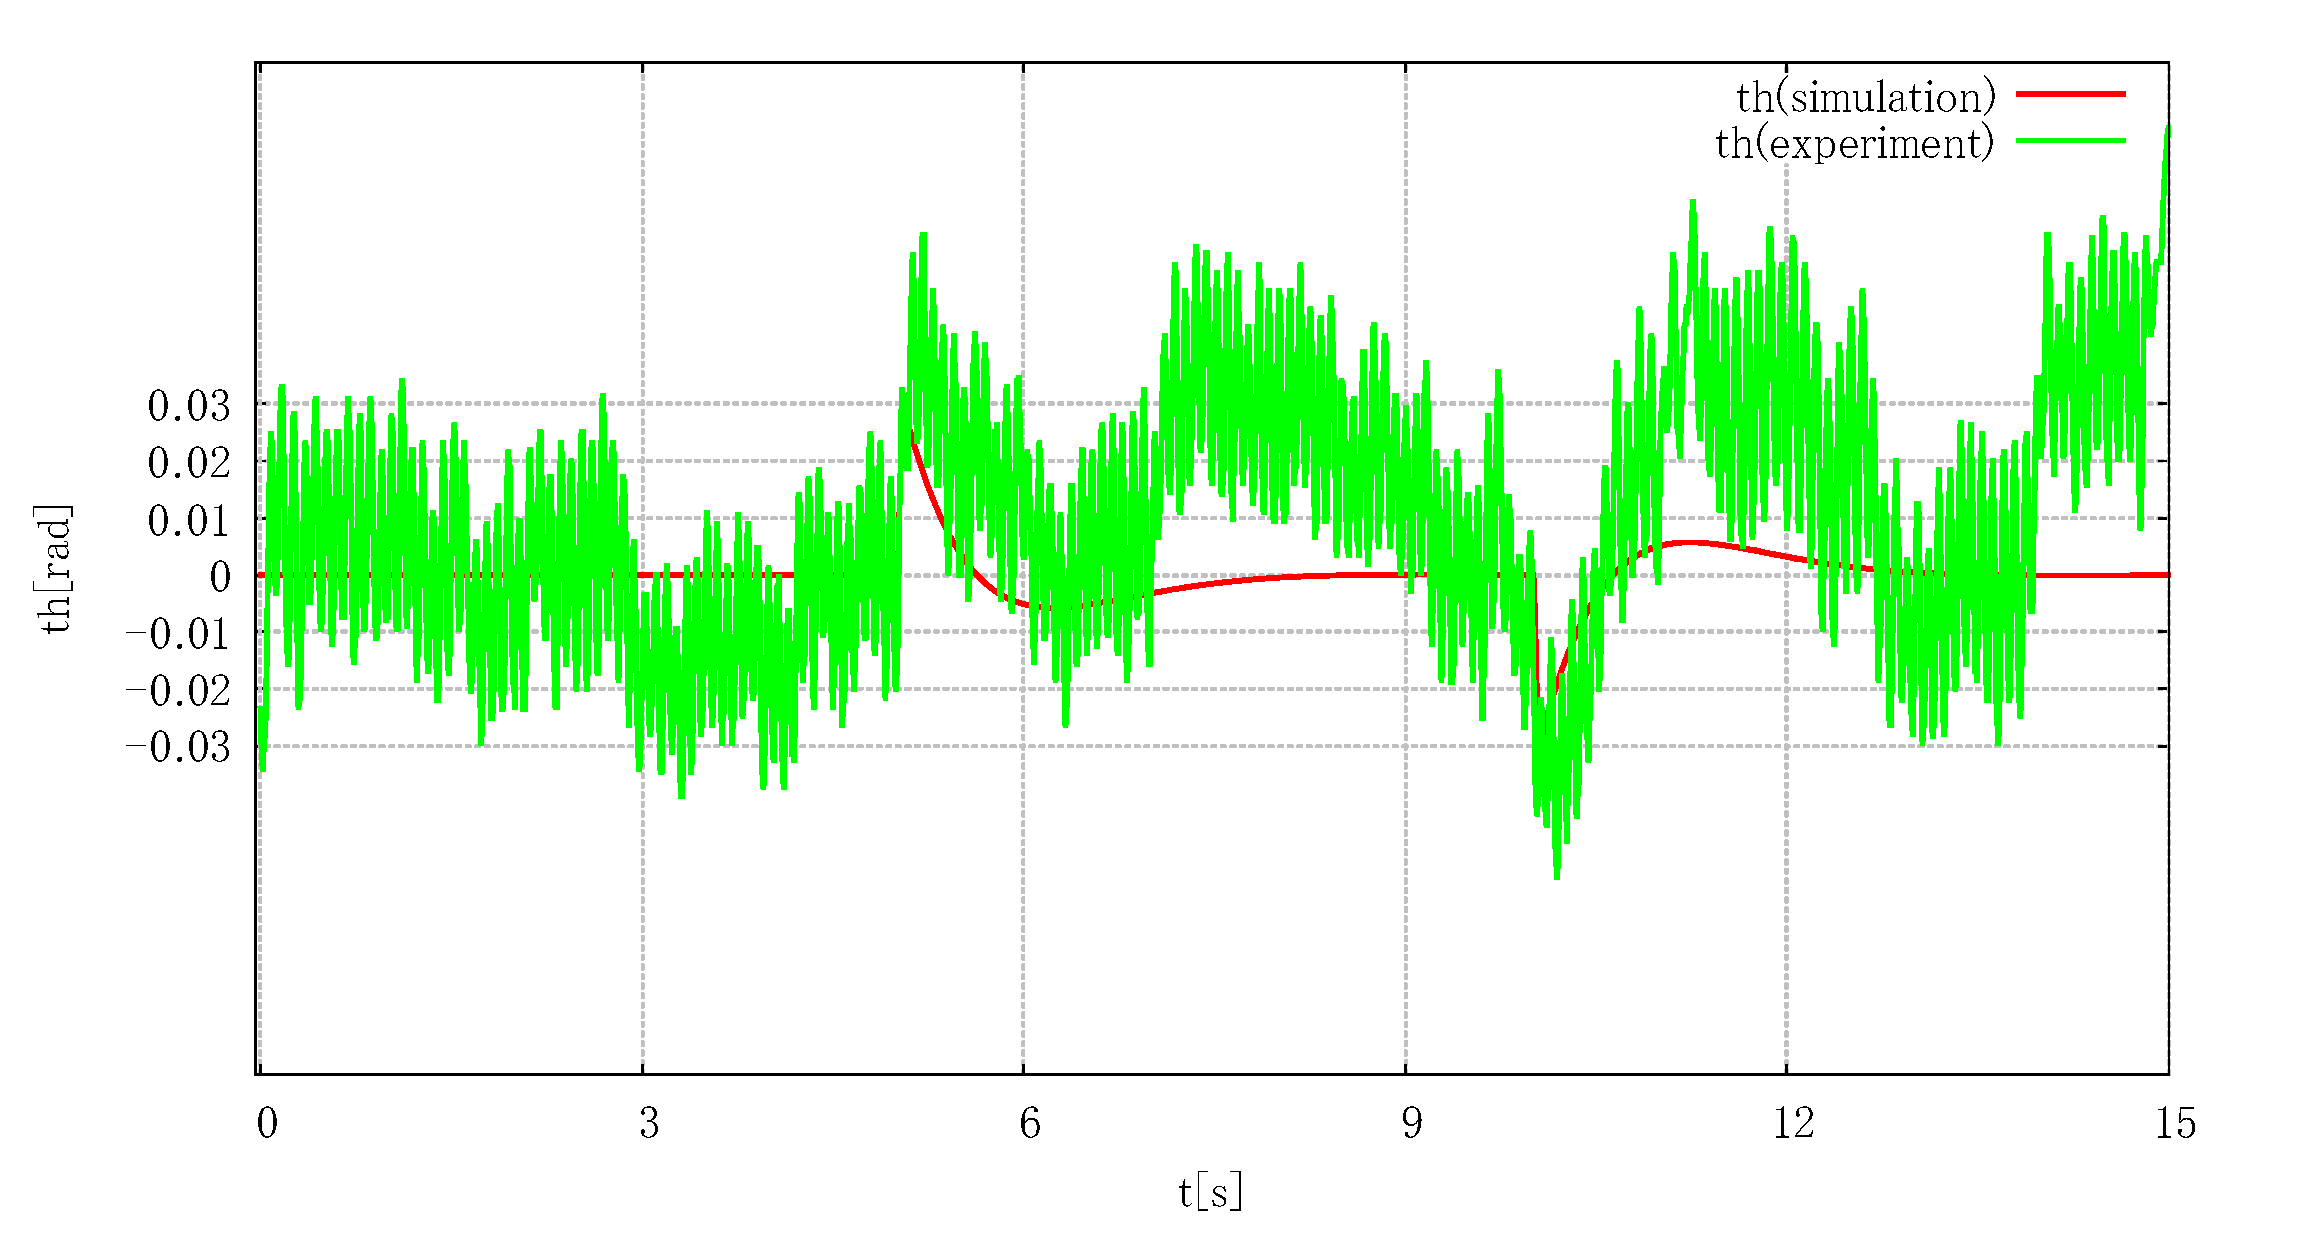
\includegraphics[width=0.49\linewidth]{gazo/experiment_Q56obs30dt05TH.eps}
		\caption{比較結果その2(左図がr,右図が$\theta$)}
		\label{image:sono2}
	\end{figure}
	\begin{figure}[H]
		\centering
		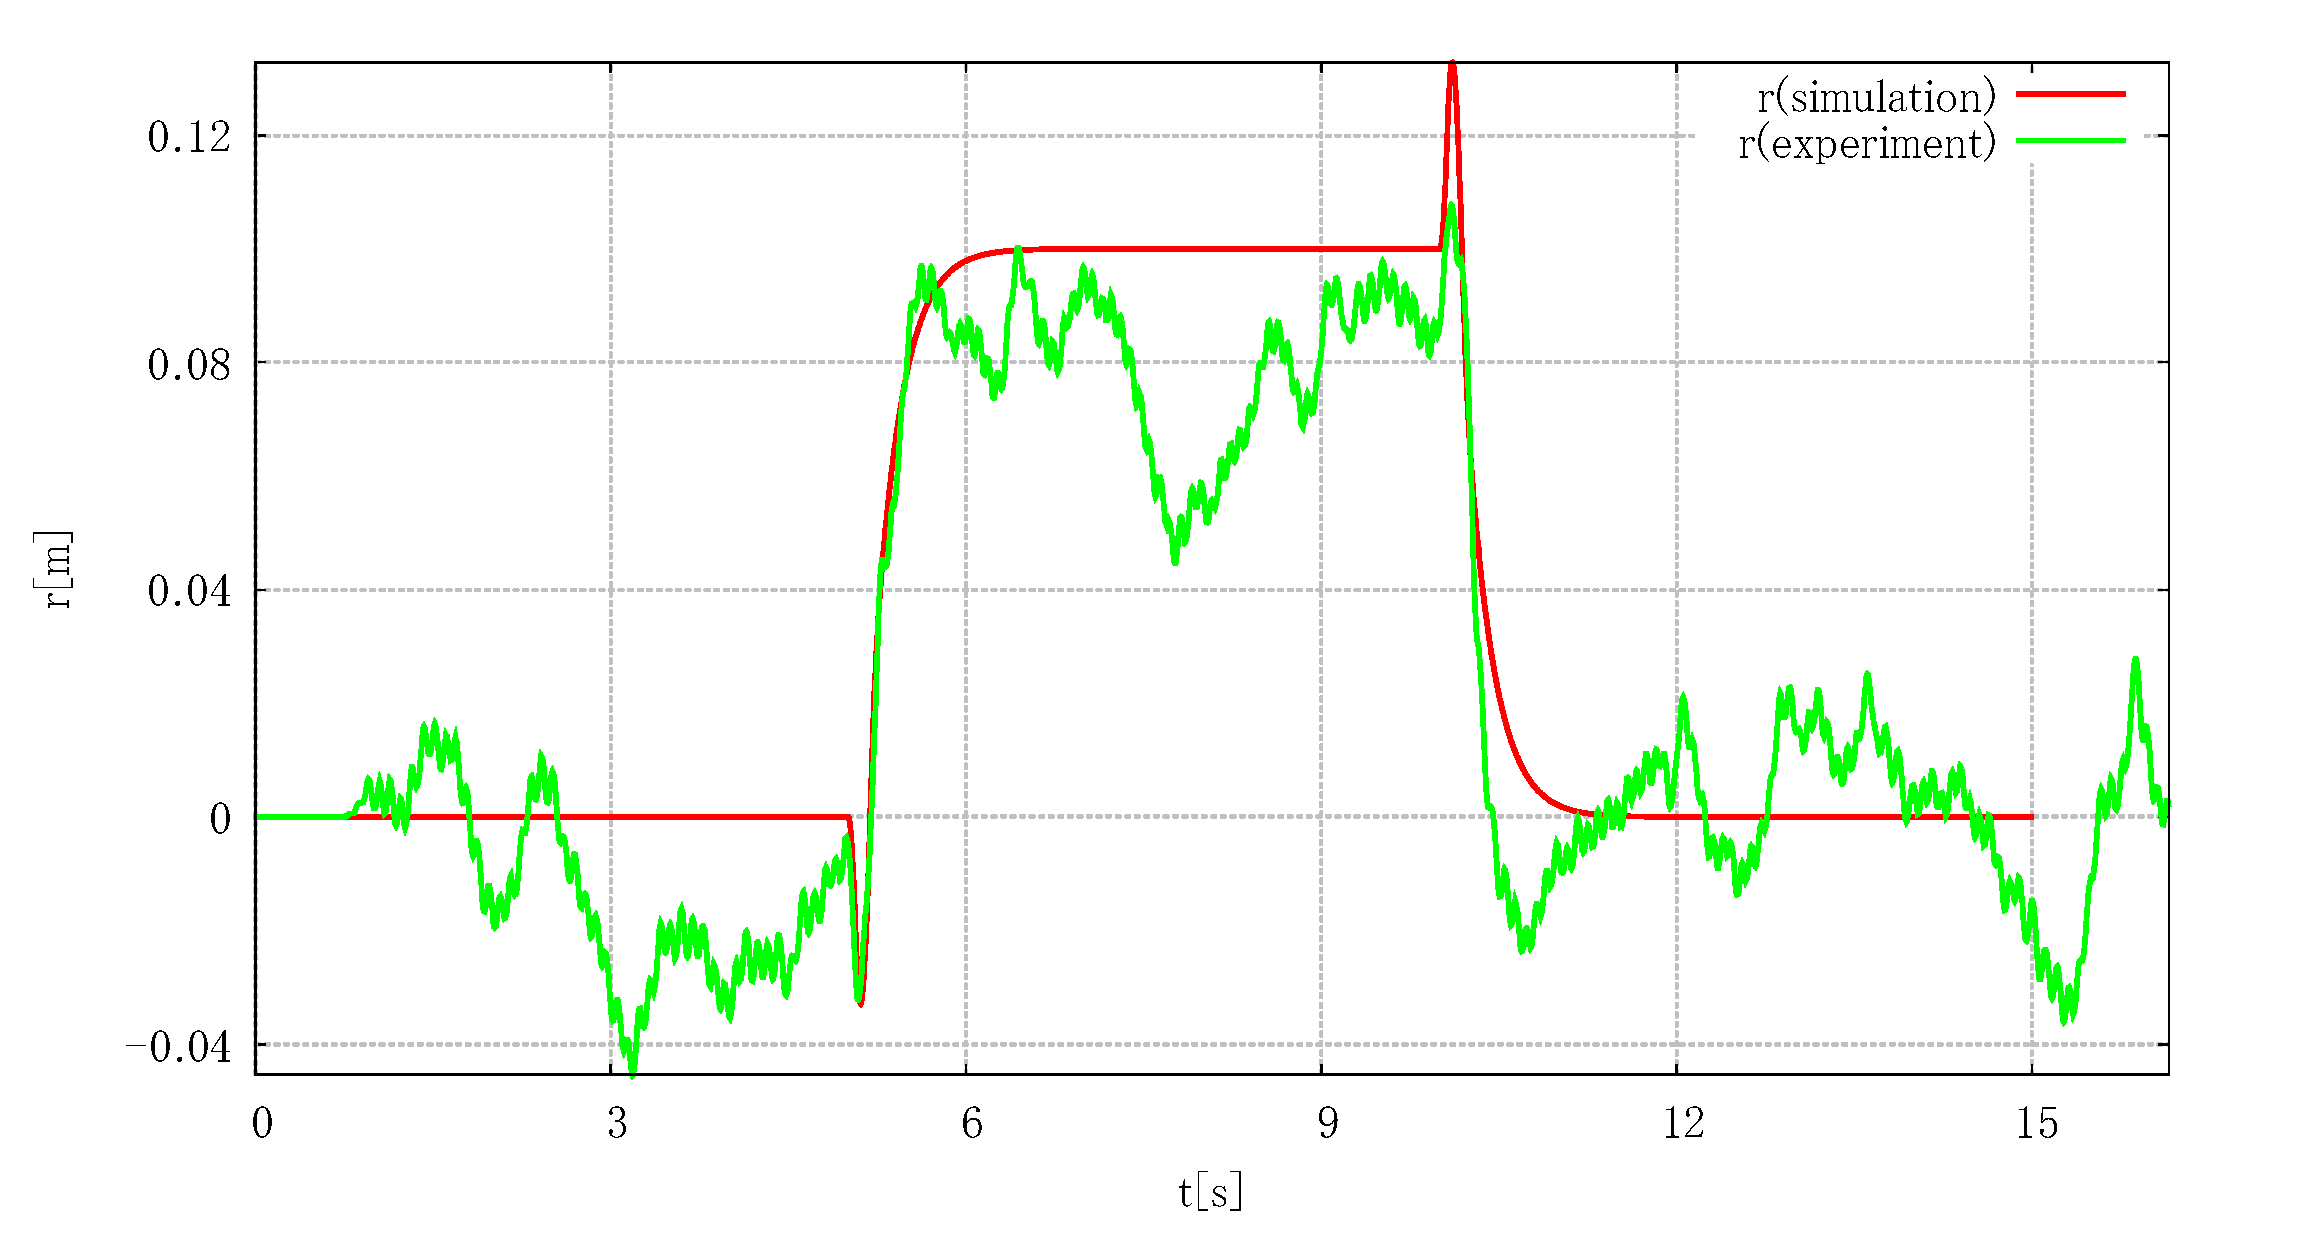
\includegraphics[width=0.49\linewidth]{gazo/experiment_Q65obs30dt05R.eps}
		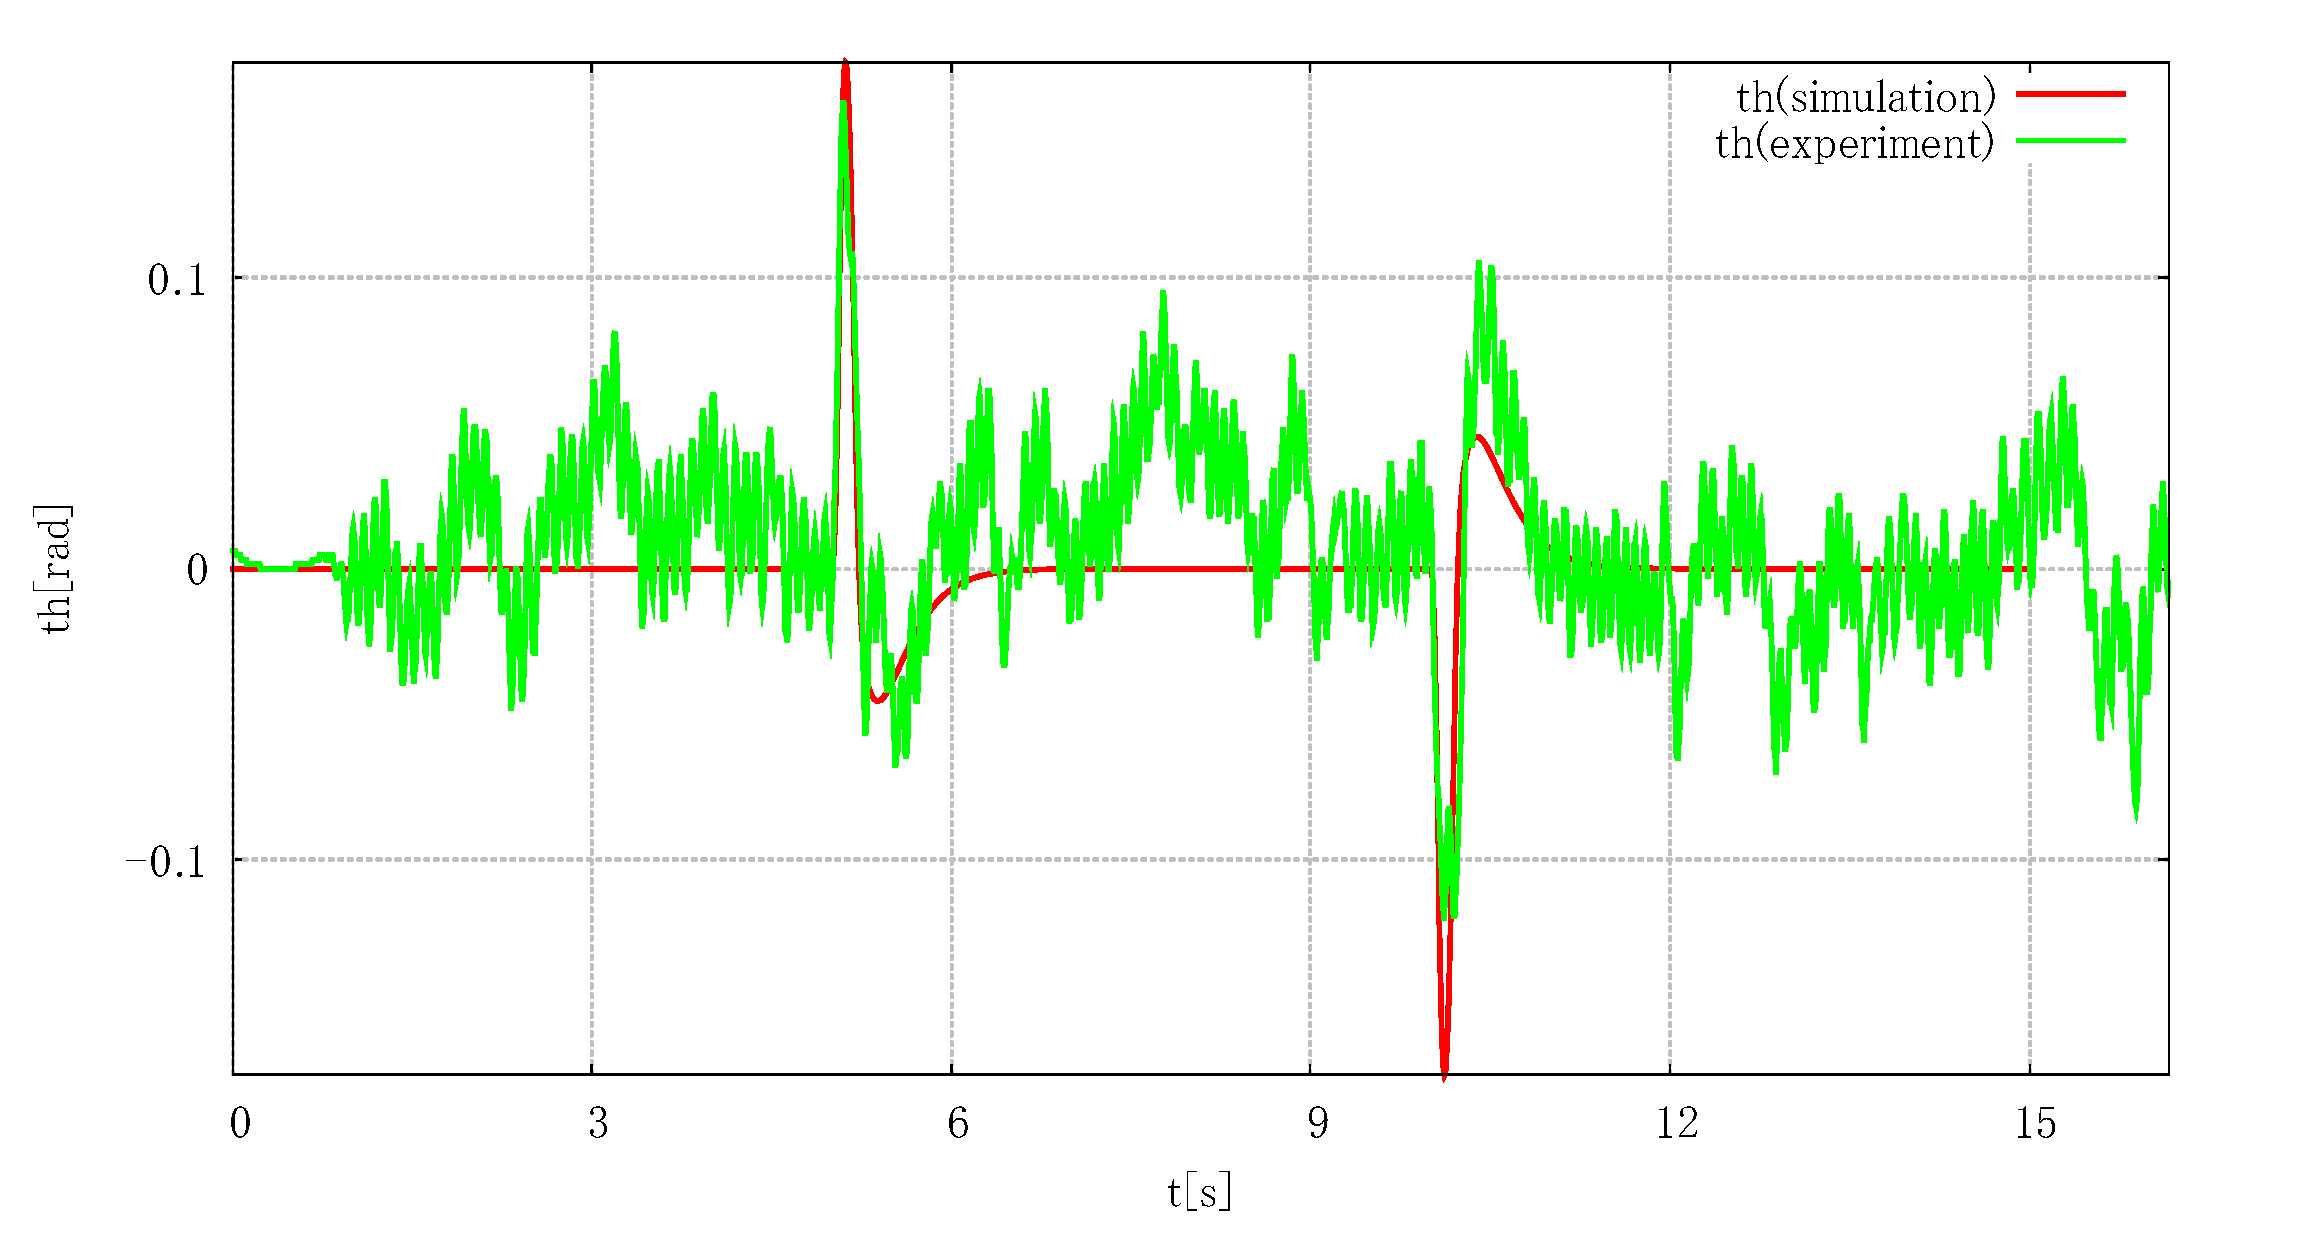
\includegraphics[width=0.49\linewidth]{gazo/experiment_Q65obs30dt05TH.eps}
		\caption{比較結果その3(左図がr,右図が$\theta$)}
		\label{image:sono3}
	\end{figure}
	\begin{figure}[H]
		\centering
		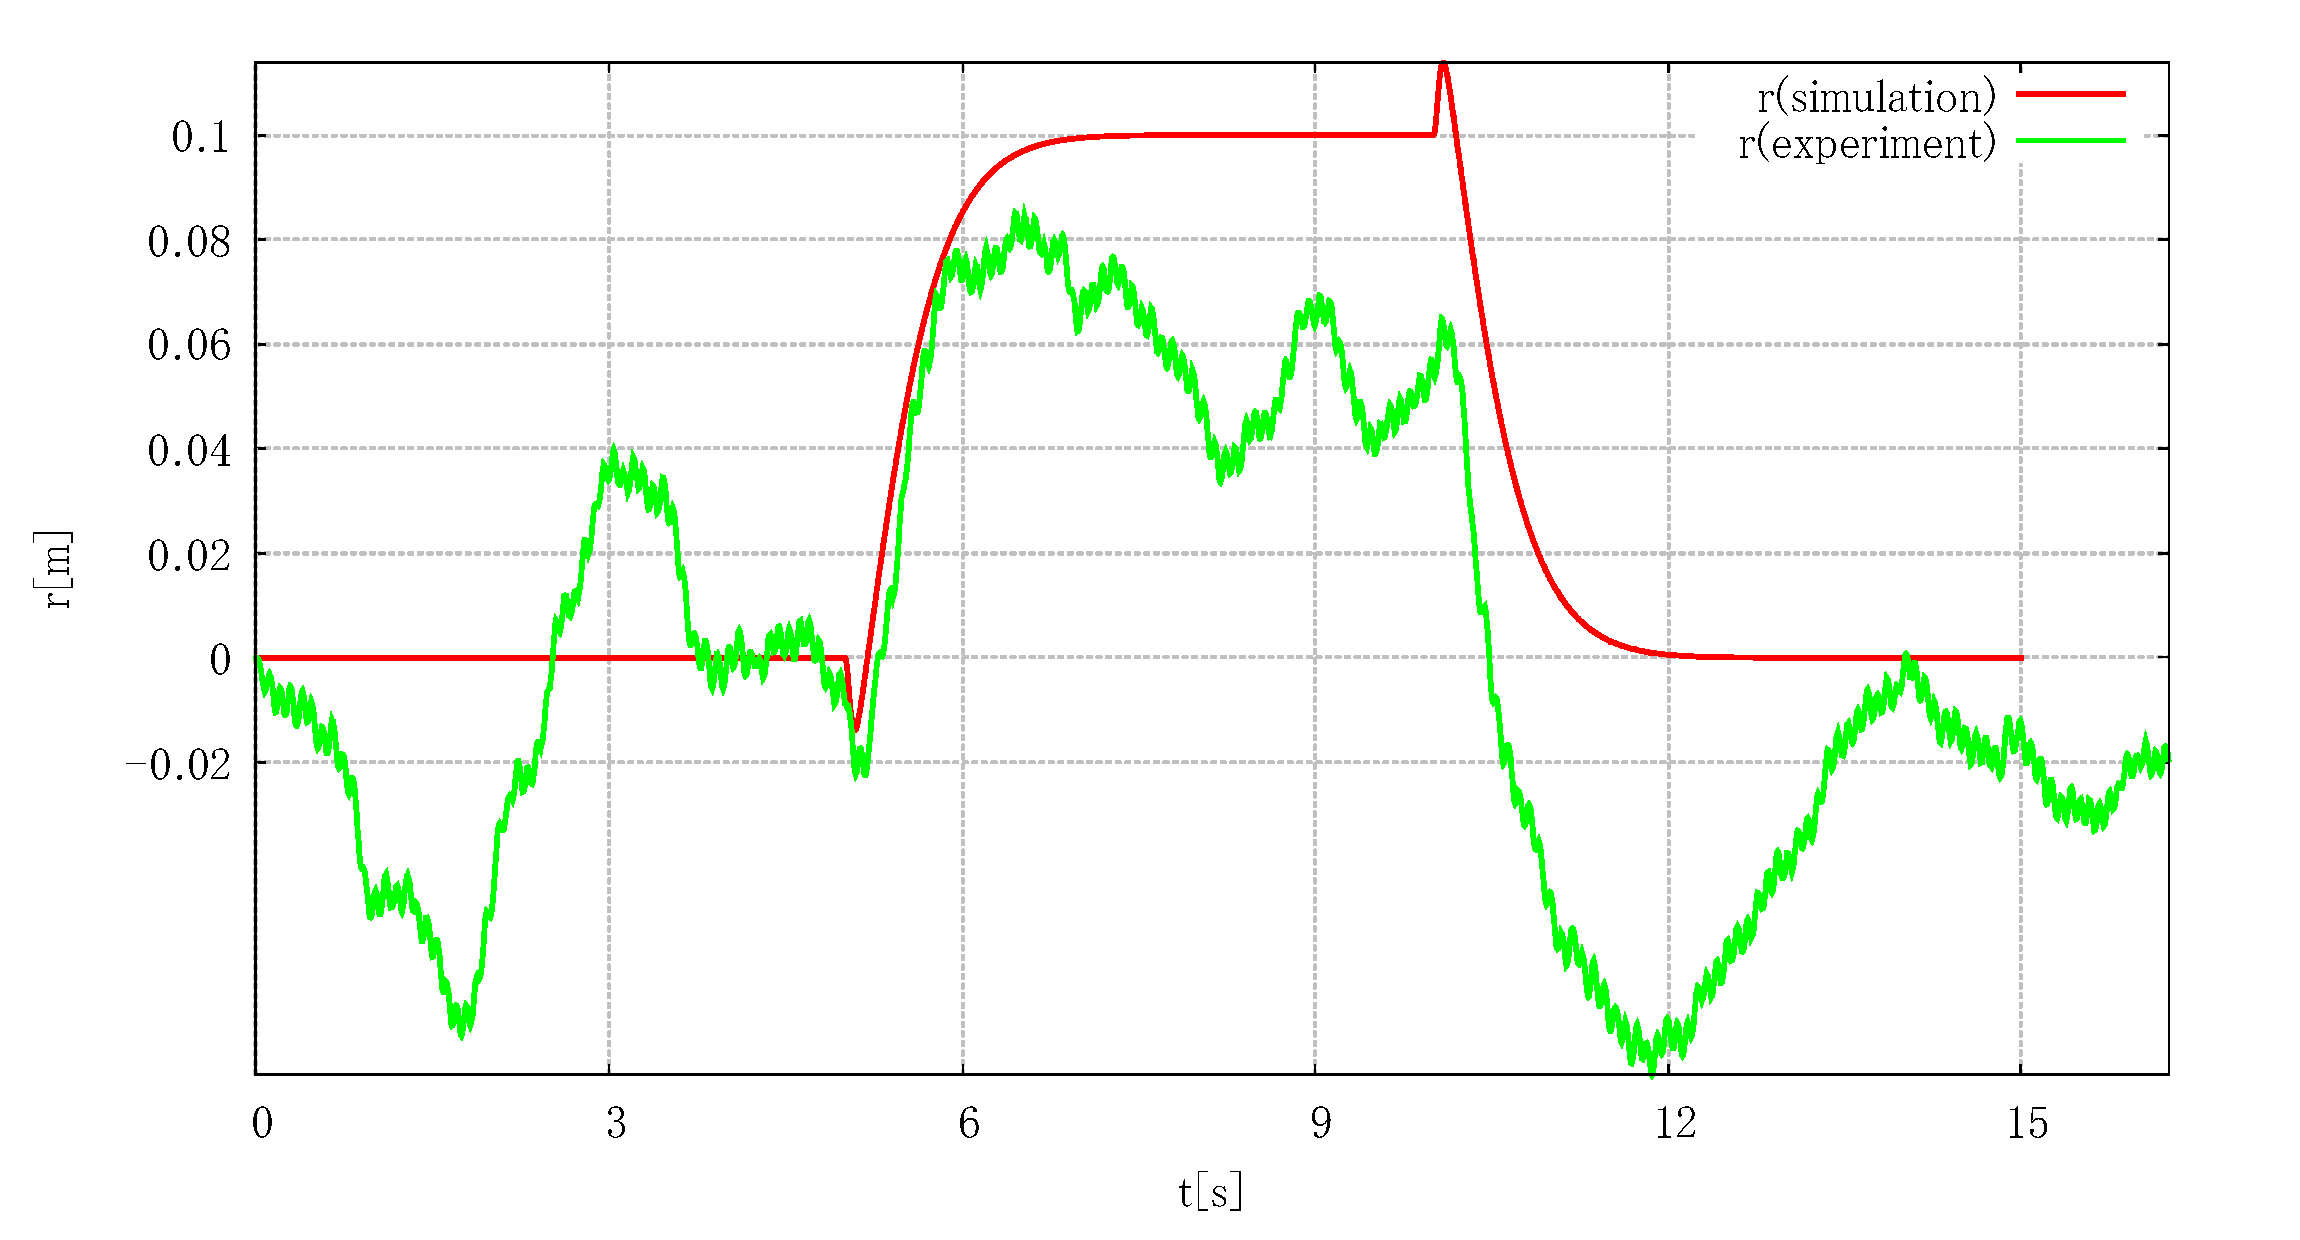
\includegraphics[width=0.49\linewidth]{gazo/experiment_Q55obs60dt05R.eps}
		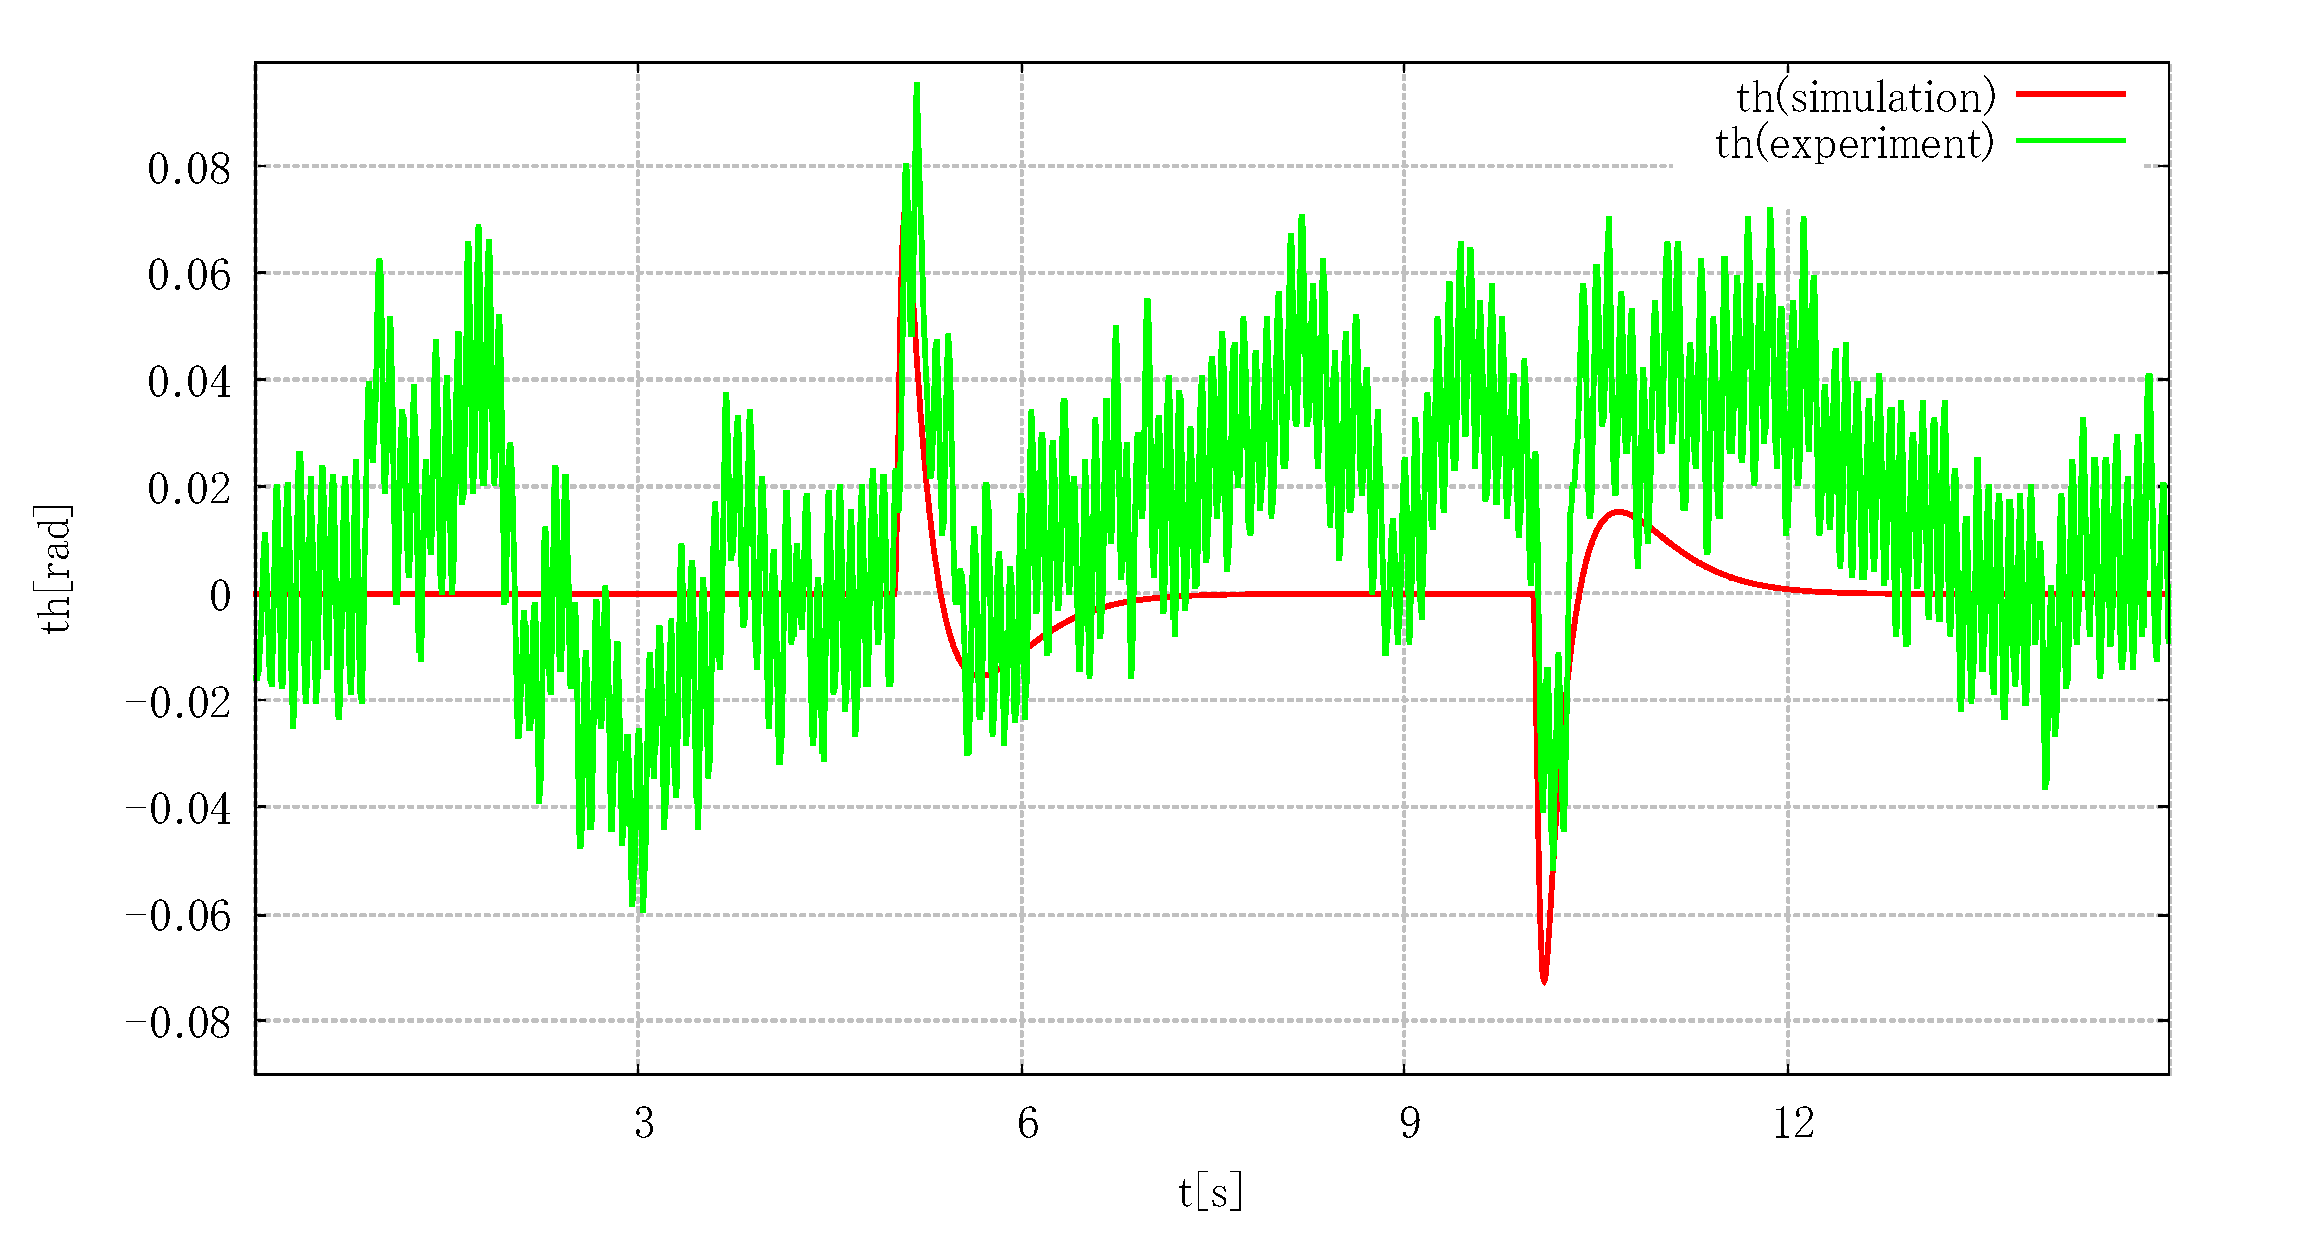
\includegraphics[width=0.49\linewidth]{gazo/experiment_Q55obs60dt05TH.eps}
		\caption{比較結果その4(左図がr,右図が$\theta$)}
		\label{image:sono4}
	\end{figure}
	\begin{figure}[H]
		\centering
		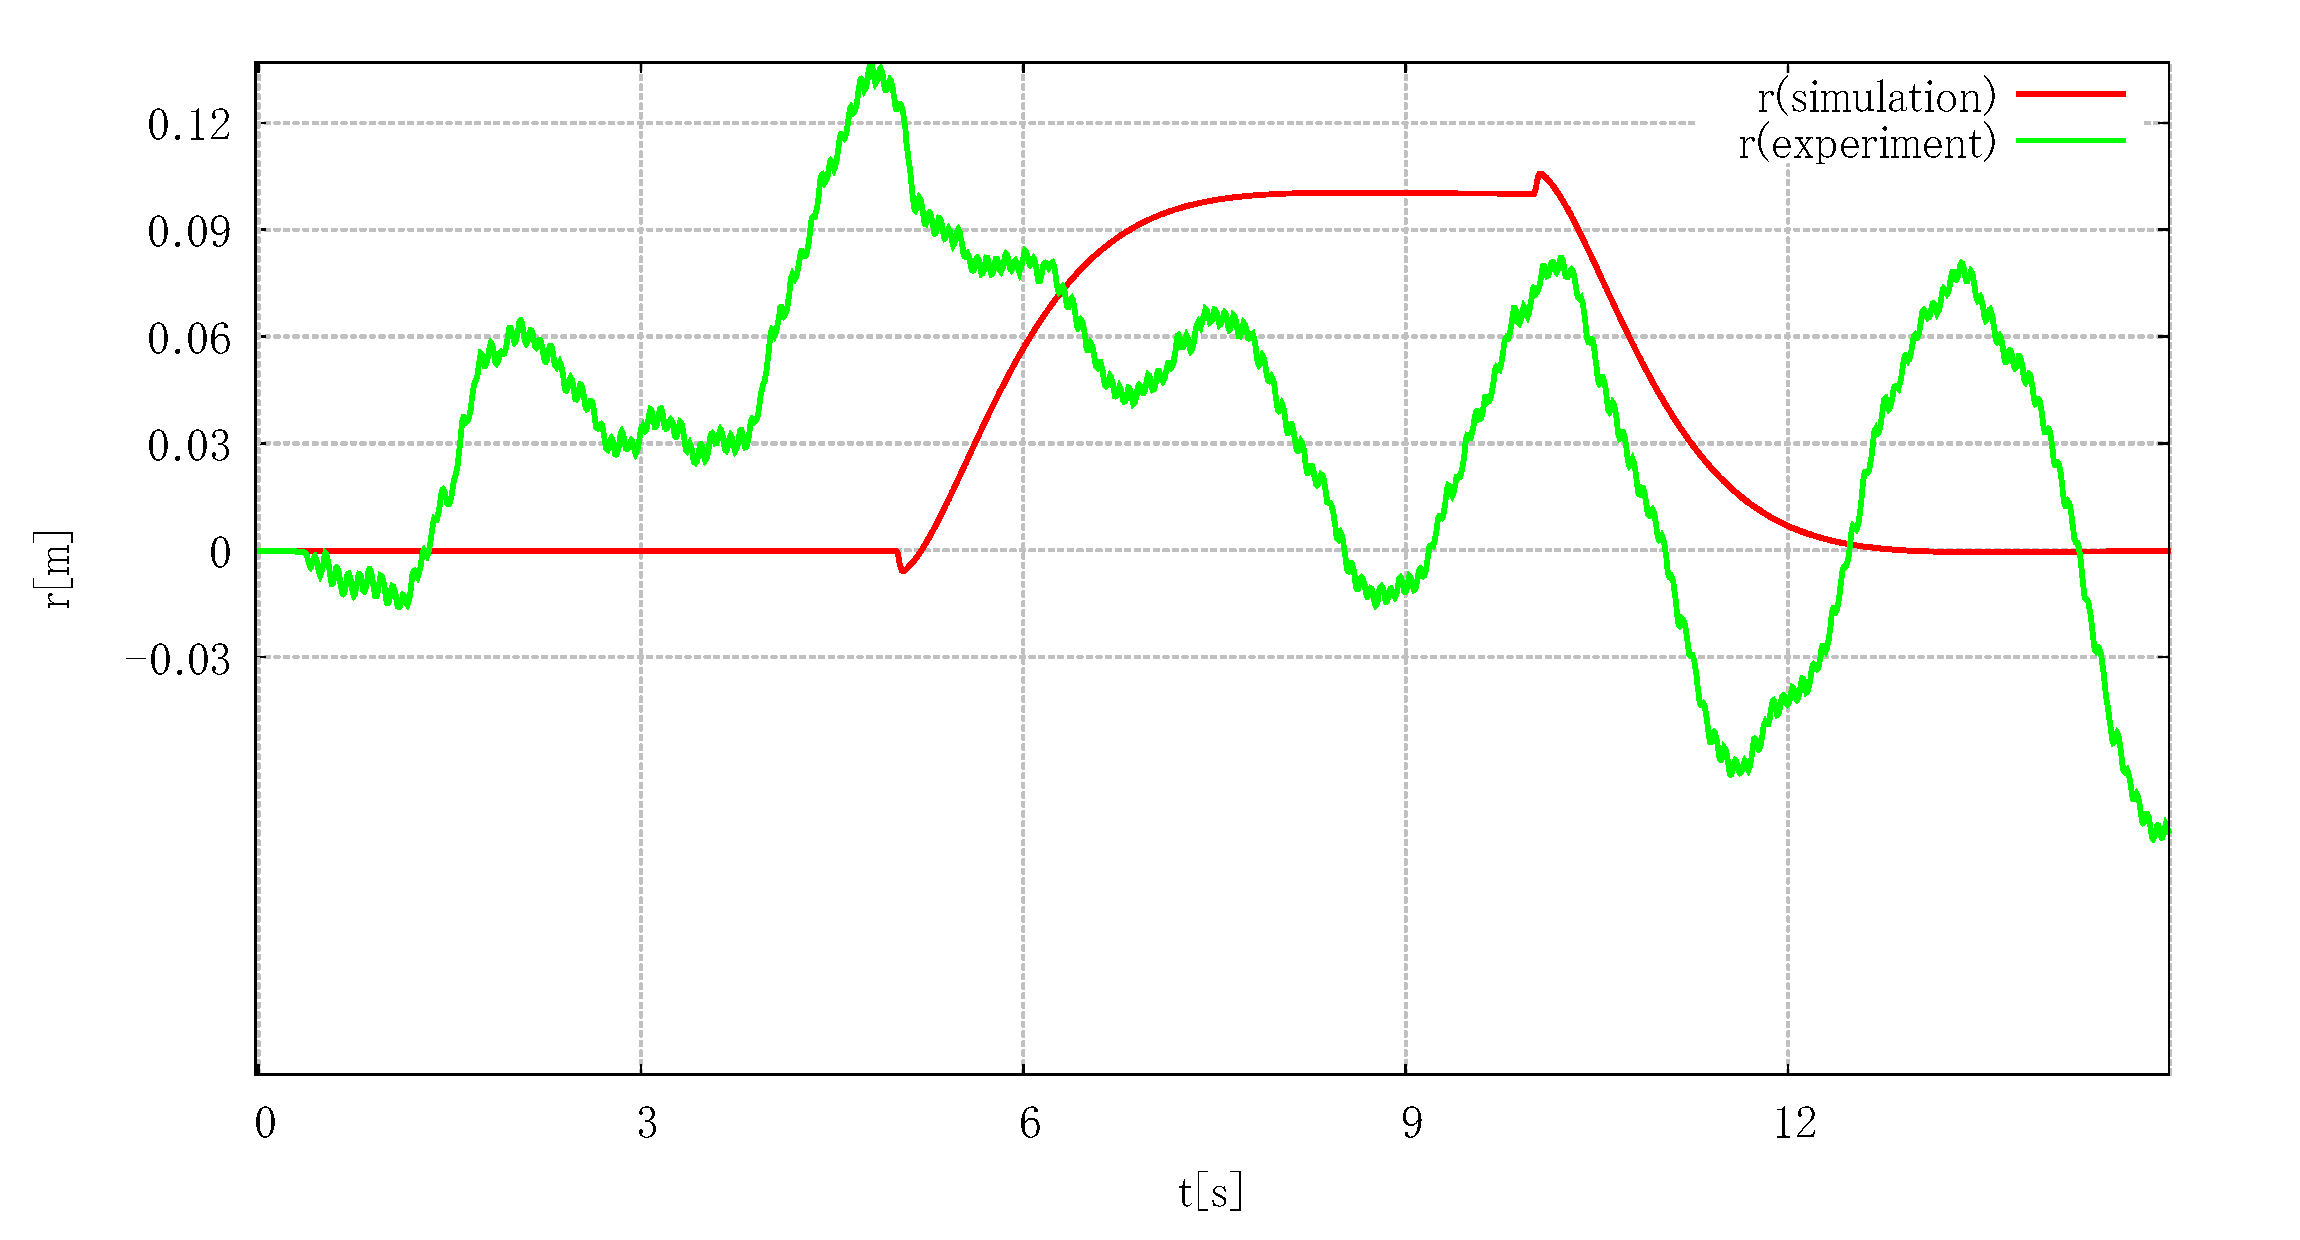
\includegraphics[width=0.49\linewidth]{gazo/experiment_Q56obs60dt05R.eps}
		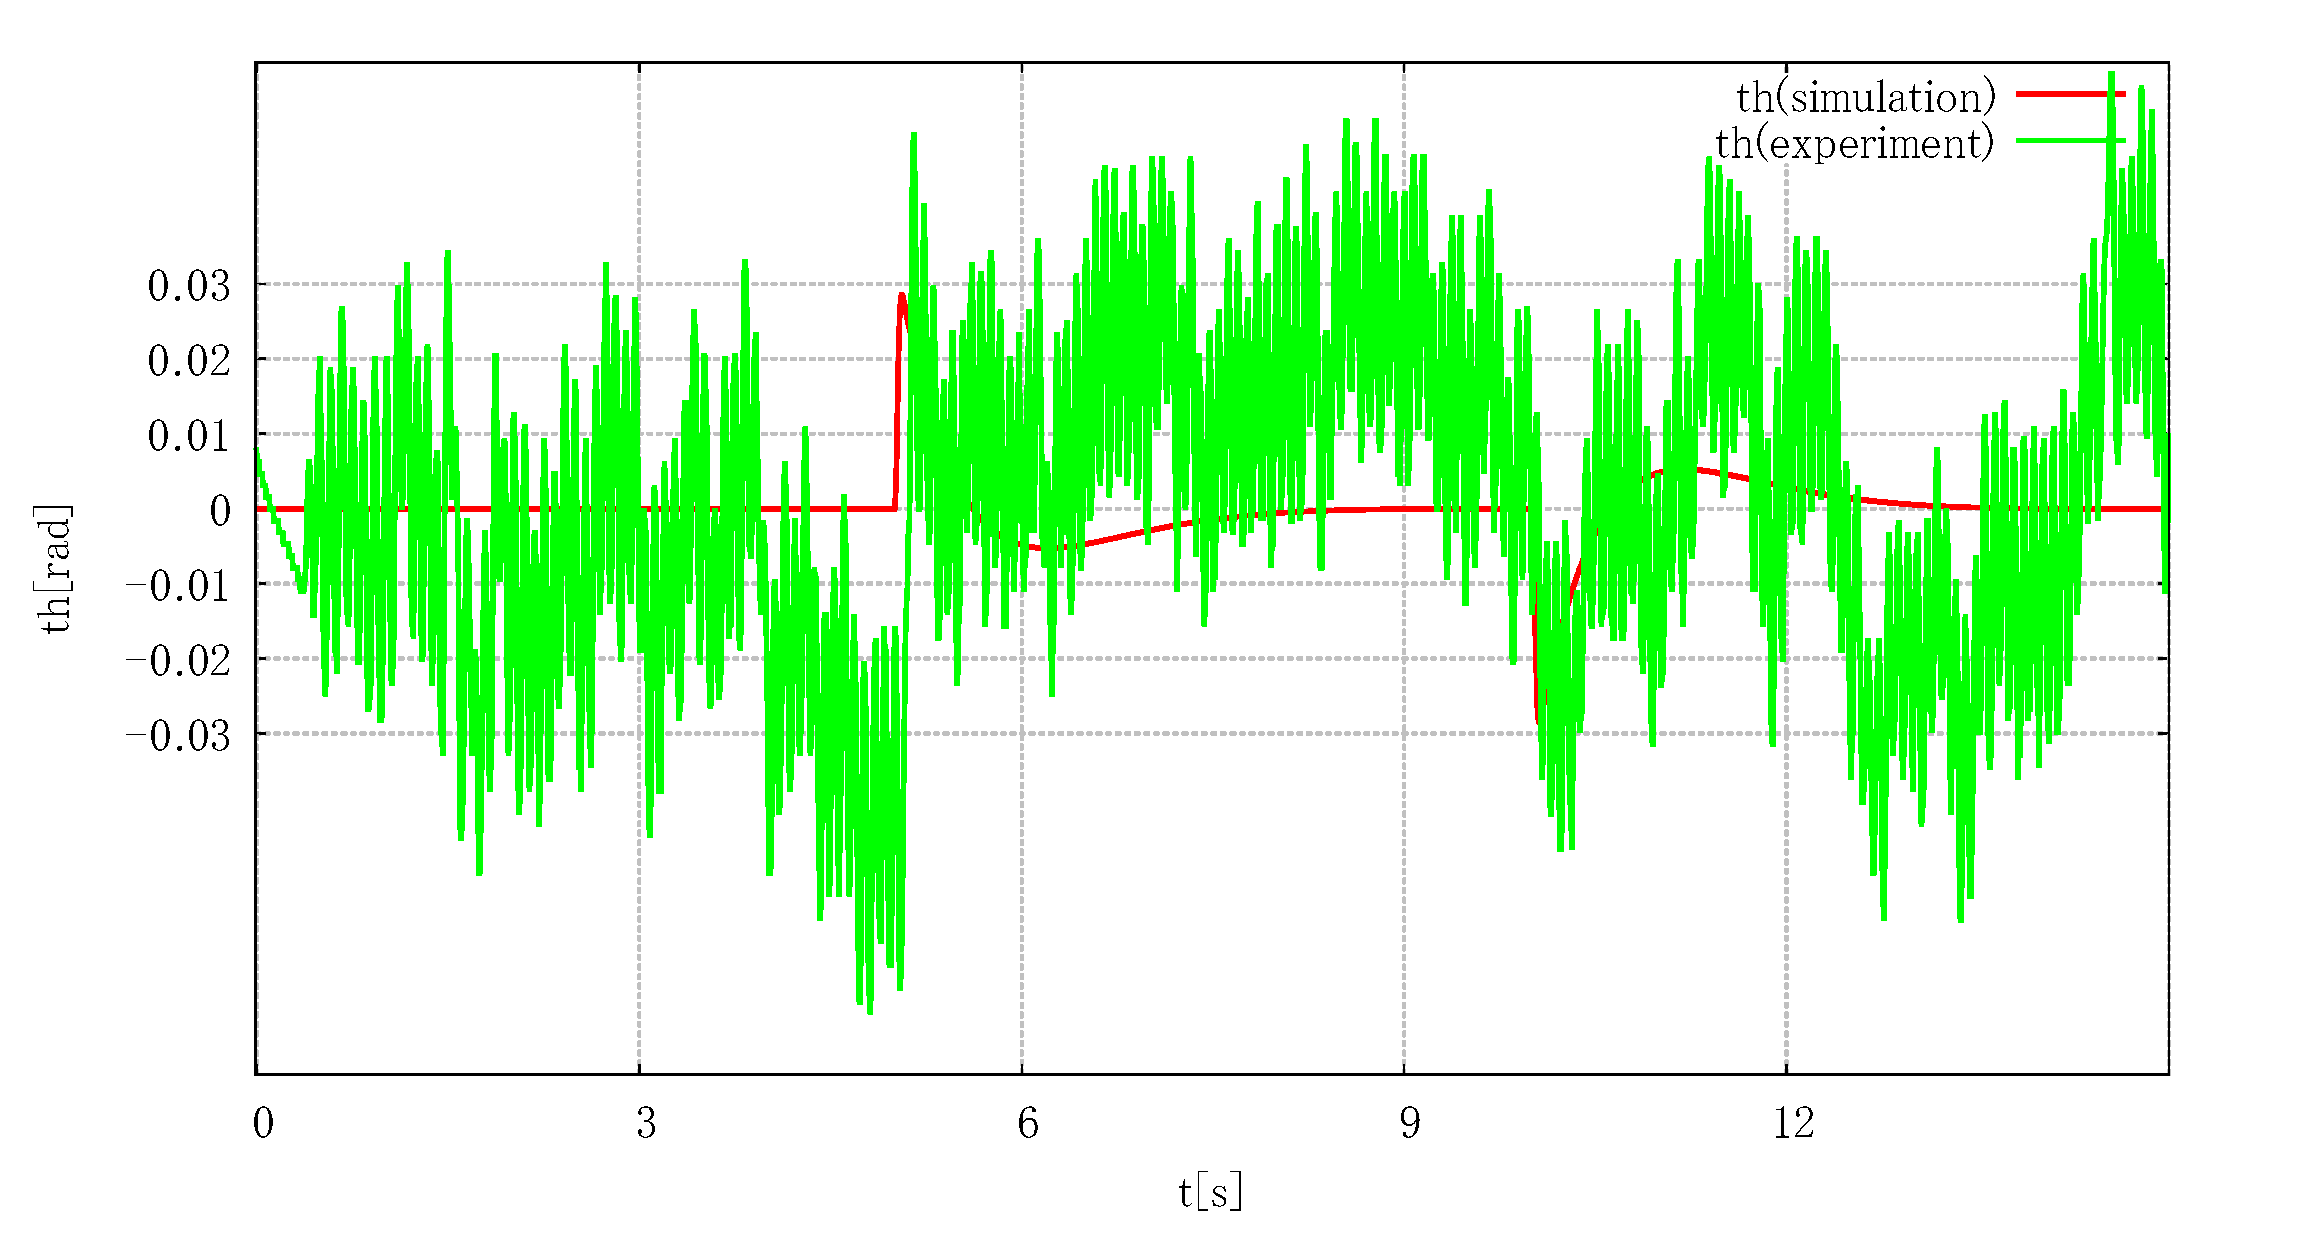
\includegraphics[width=0.49\linewidth]{gazo/experiment_Q56obs60dt05TH.eps}
		\caption{比較結果その5(左図がr,右図が$\theta$)}
		\label{image:sono5}
	\end{figure}
	\begin{figure}[H]
		\centering
		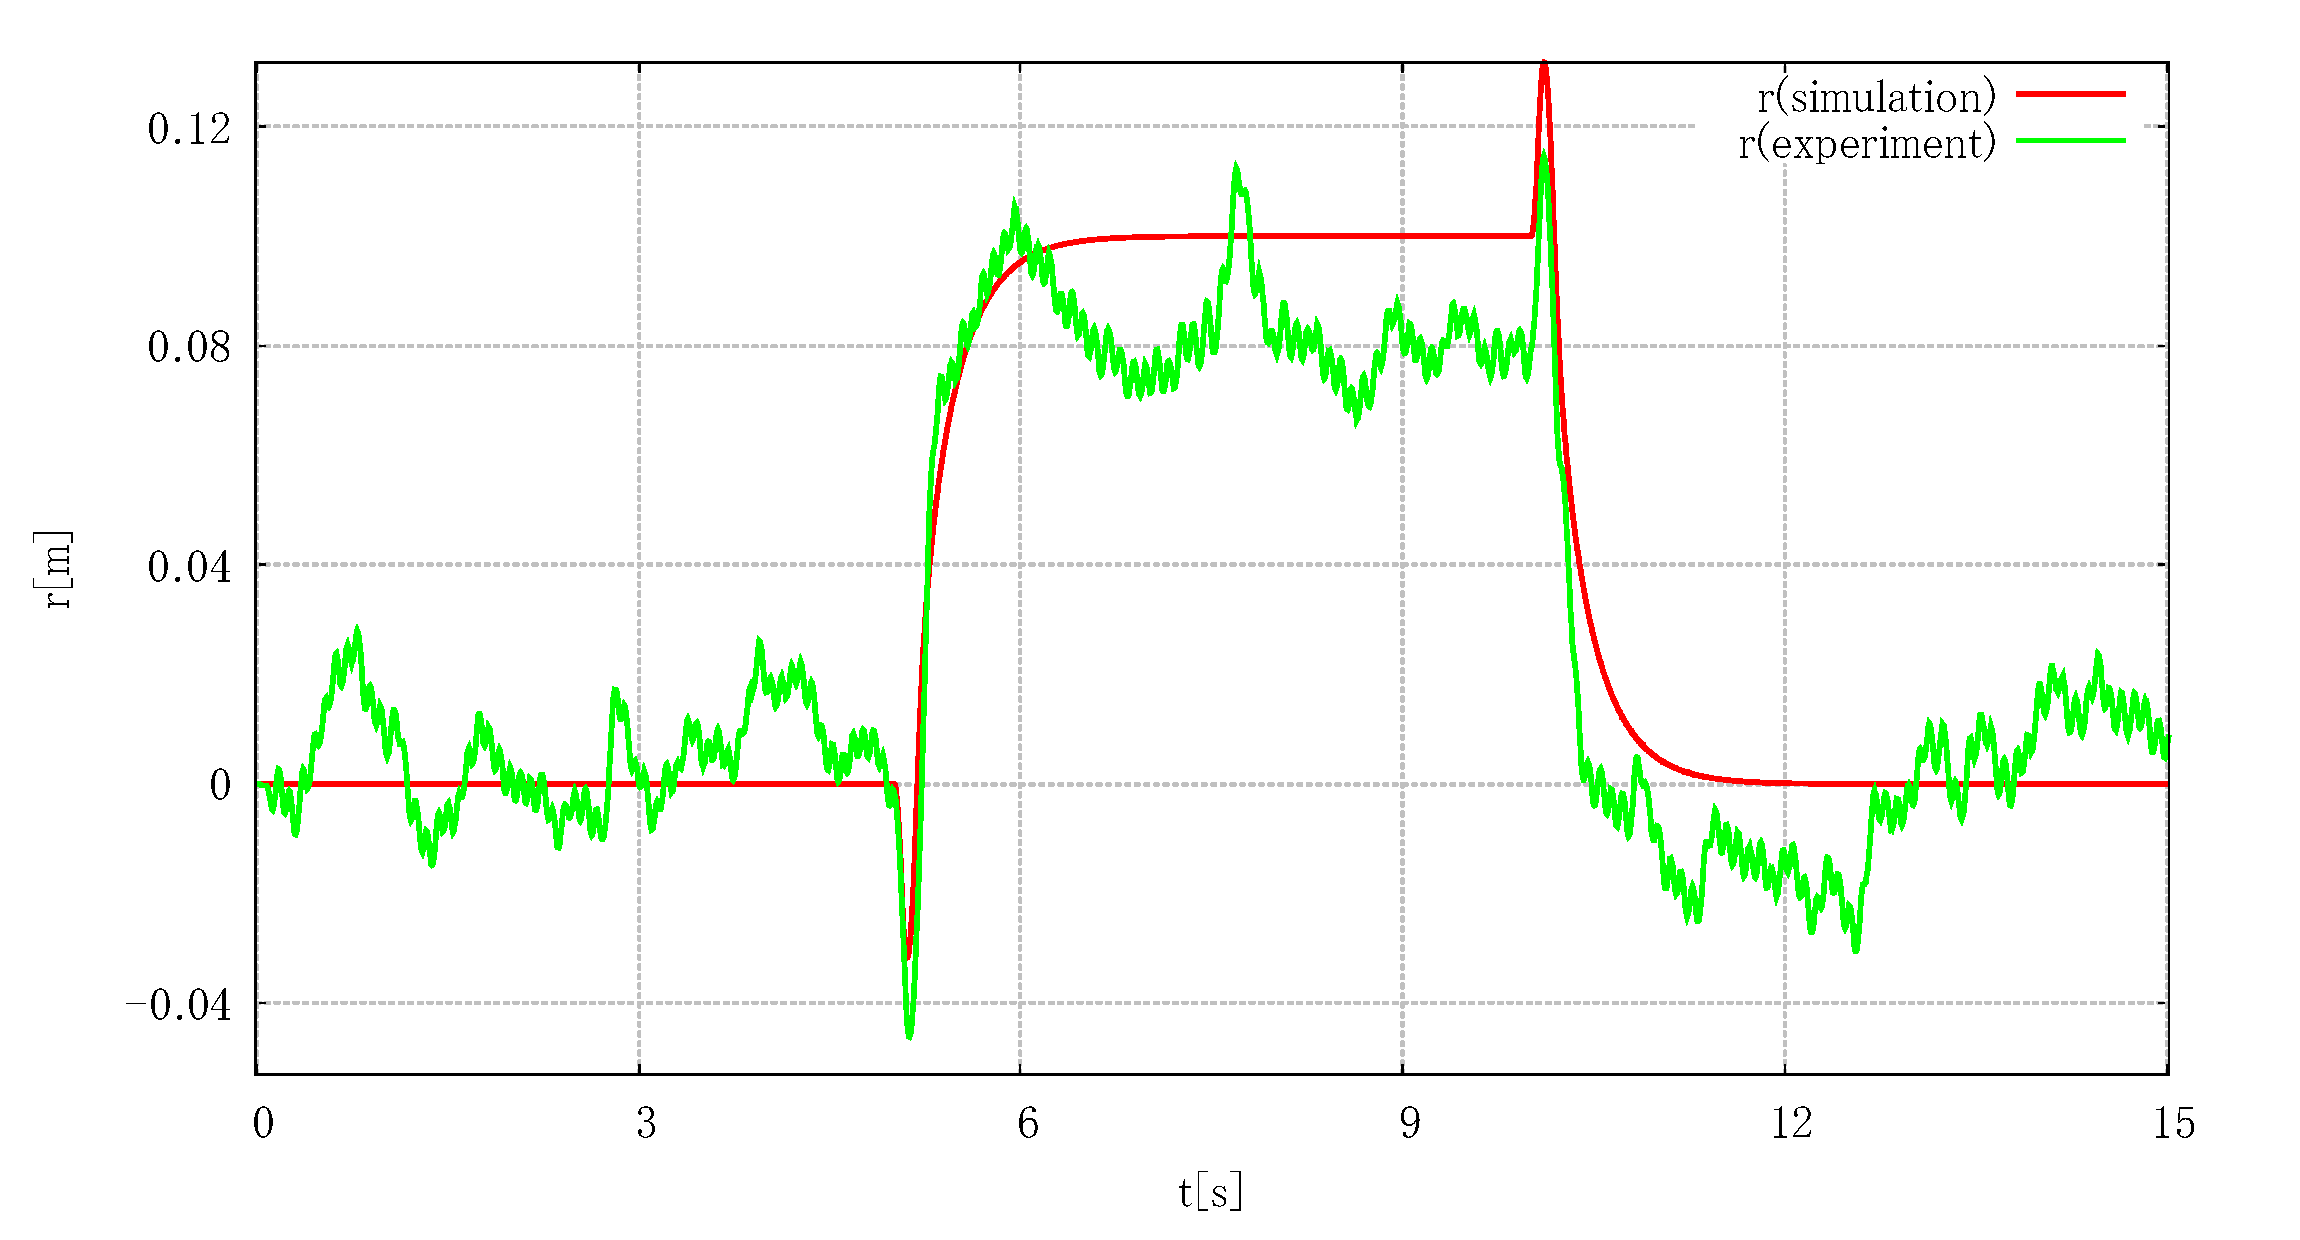
\includegraphics[width=0.49\linewidth]{gazo/experiment_Q65obs60dt05R.eps}
		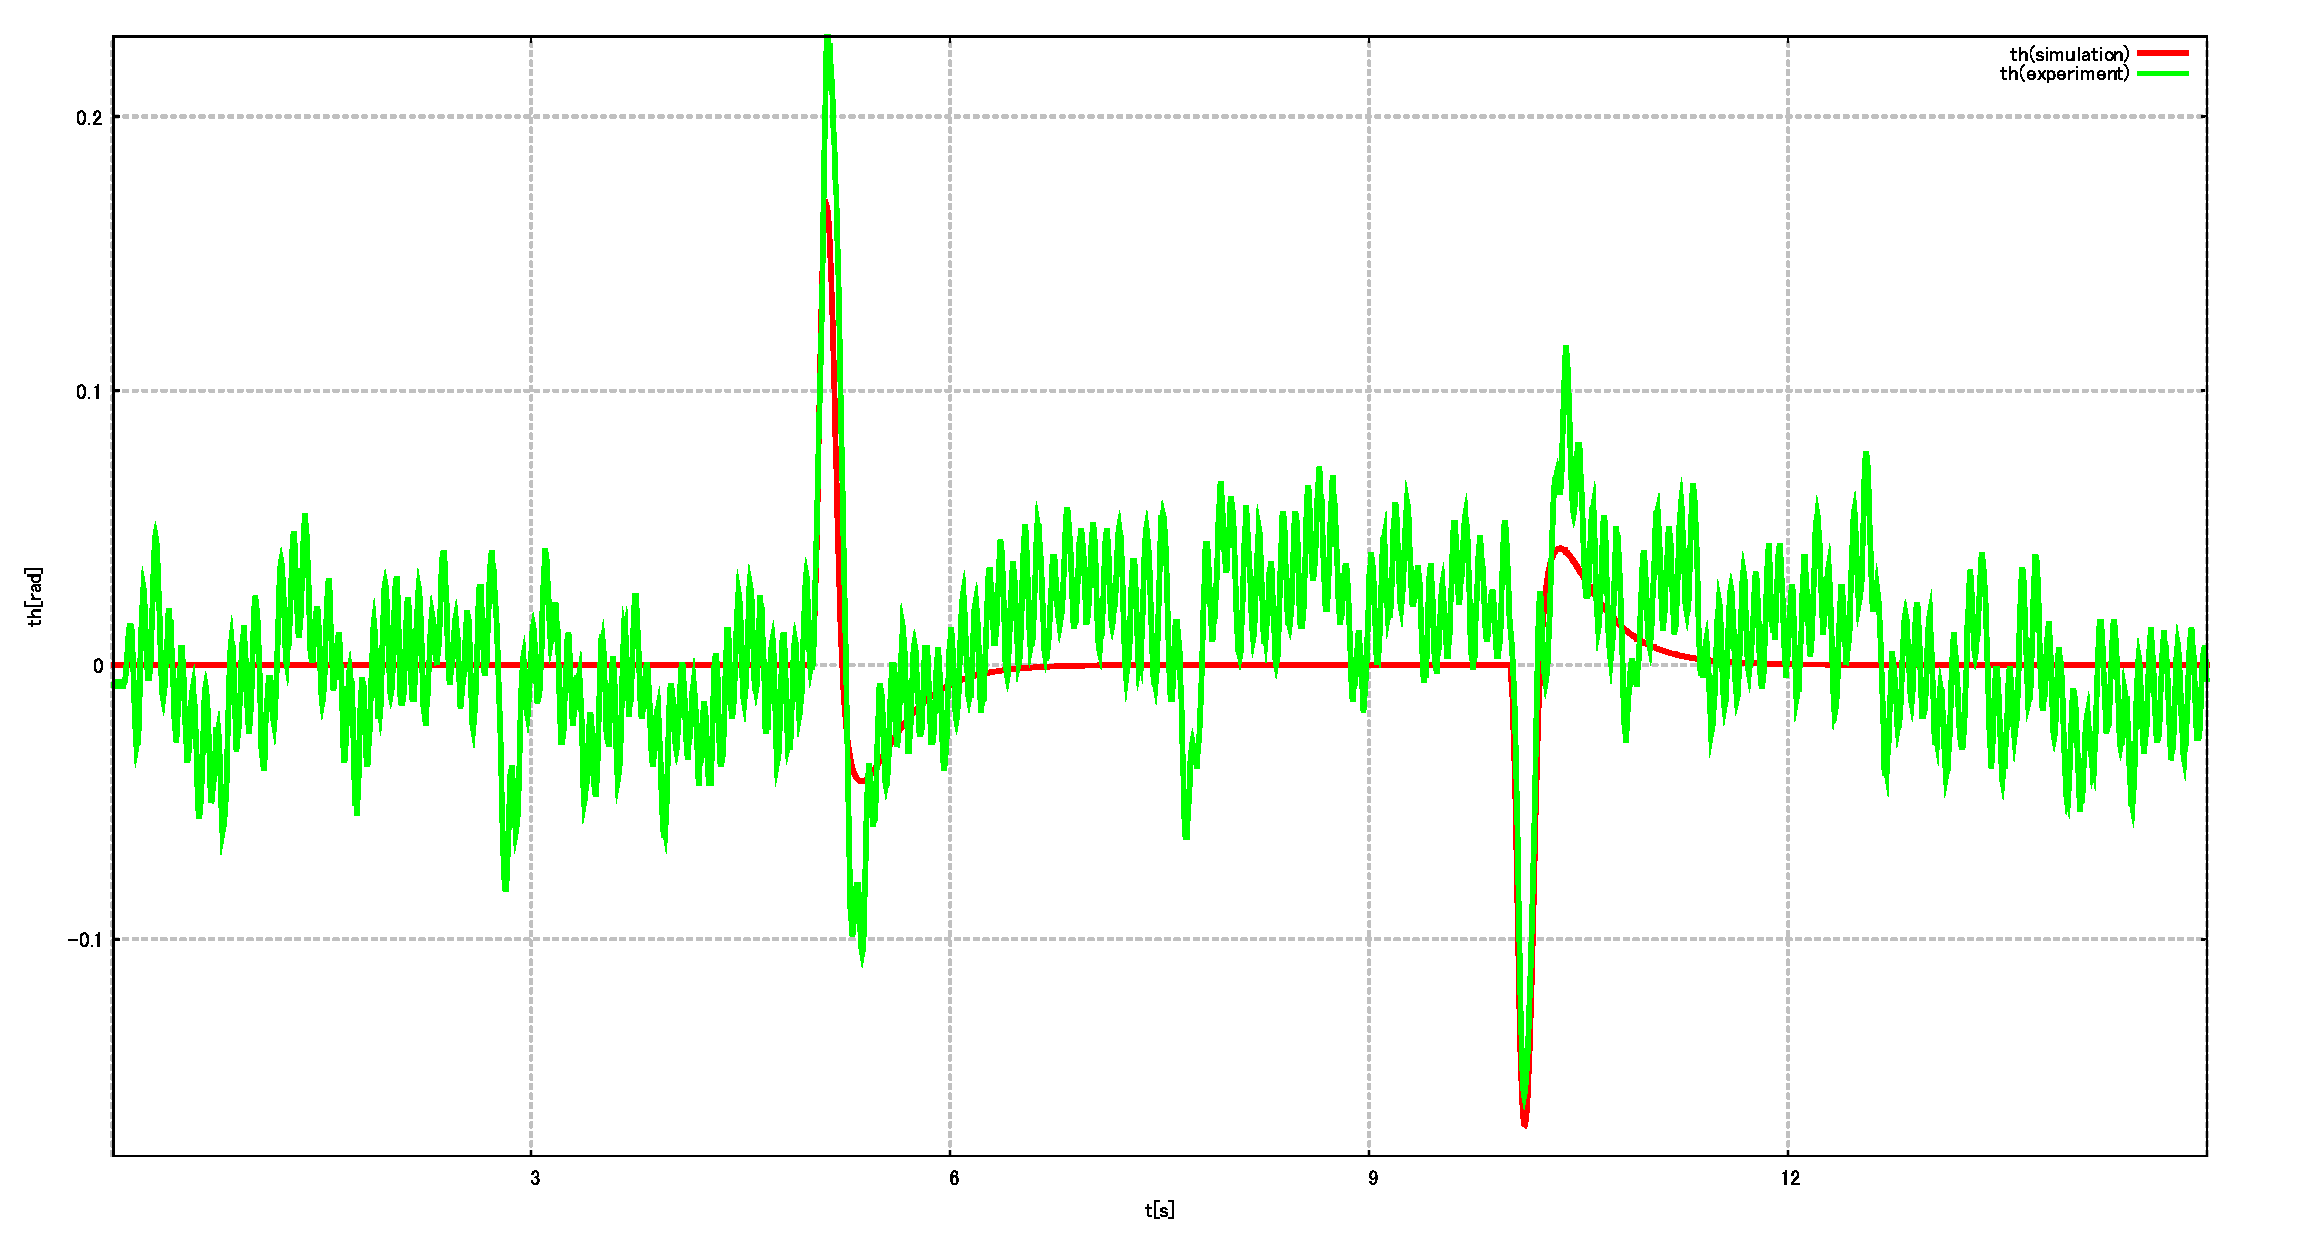
\includegraphics[width=0.49\linewidth]{gazo/experiment_Q65obs60dt05TH.eps}
		\caption{比較結果その6(左図がr,右図が$\theta$)}
		\label{image:sono6}
	\end{figure}
	\begin{figure}[H]
		\centering
		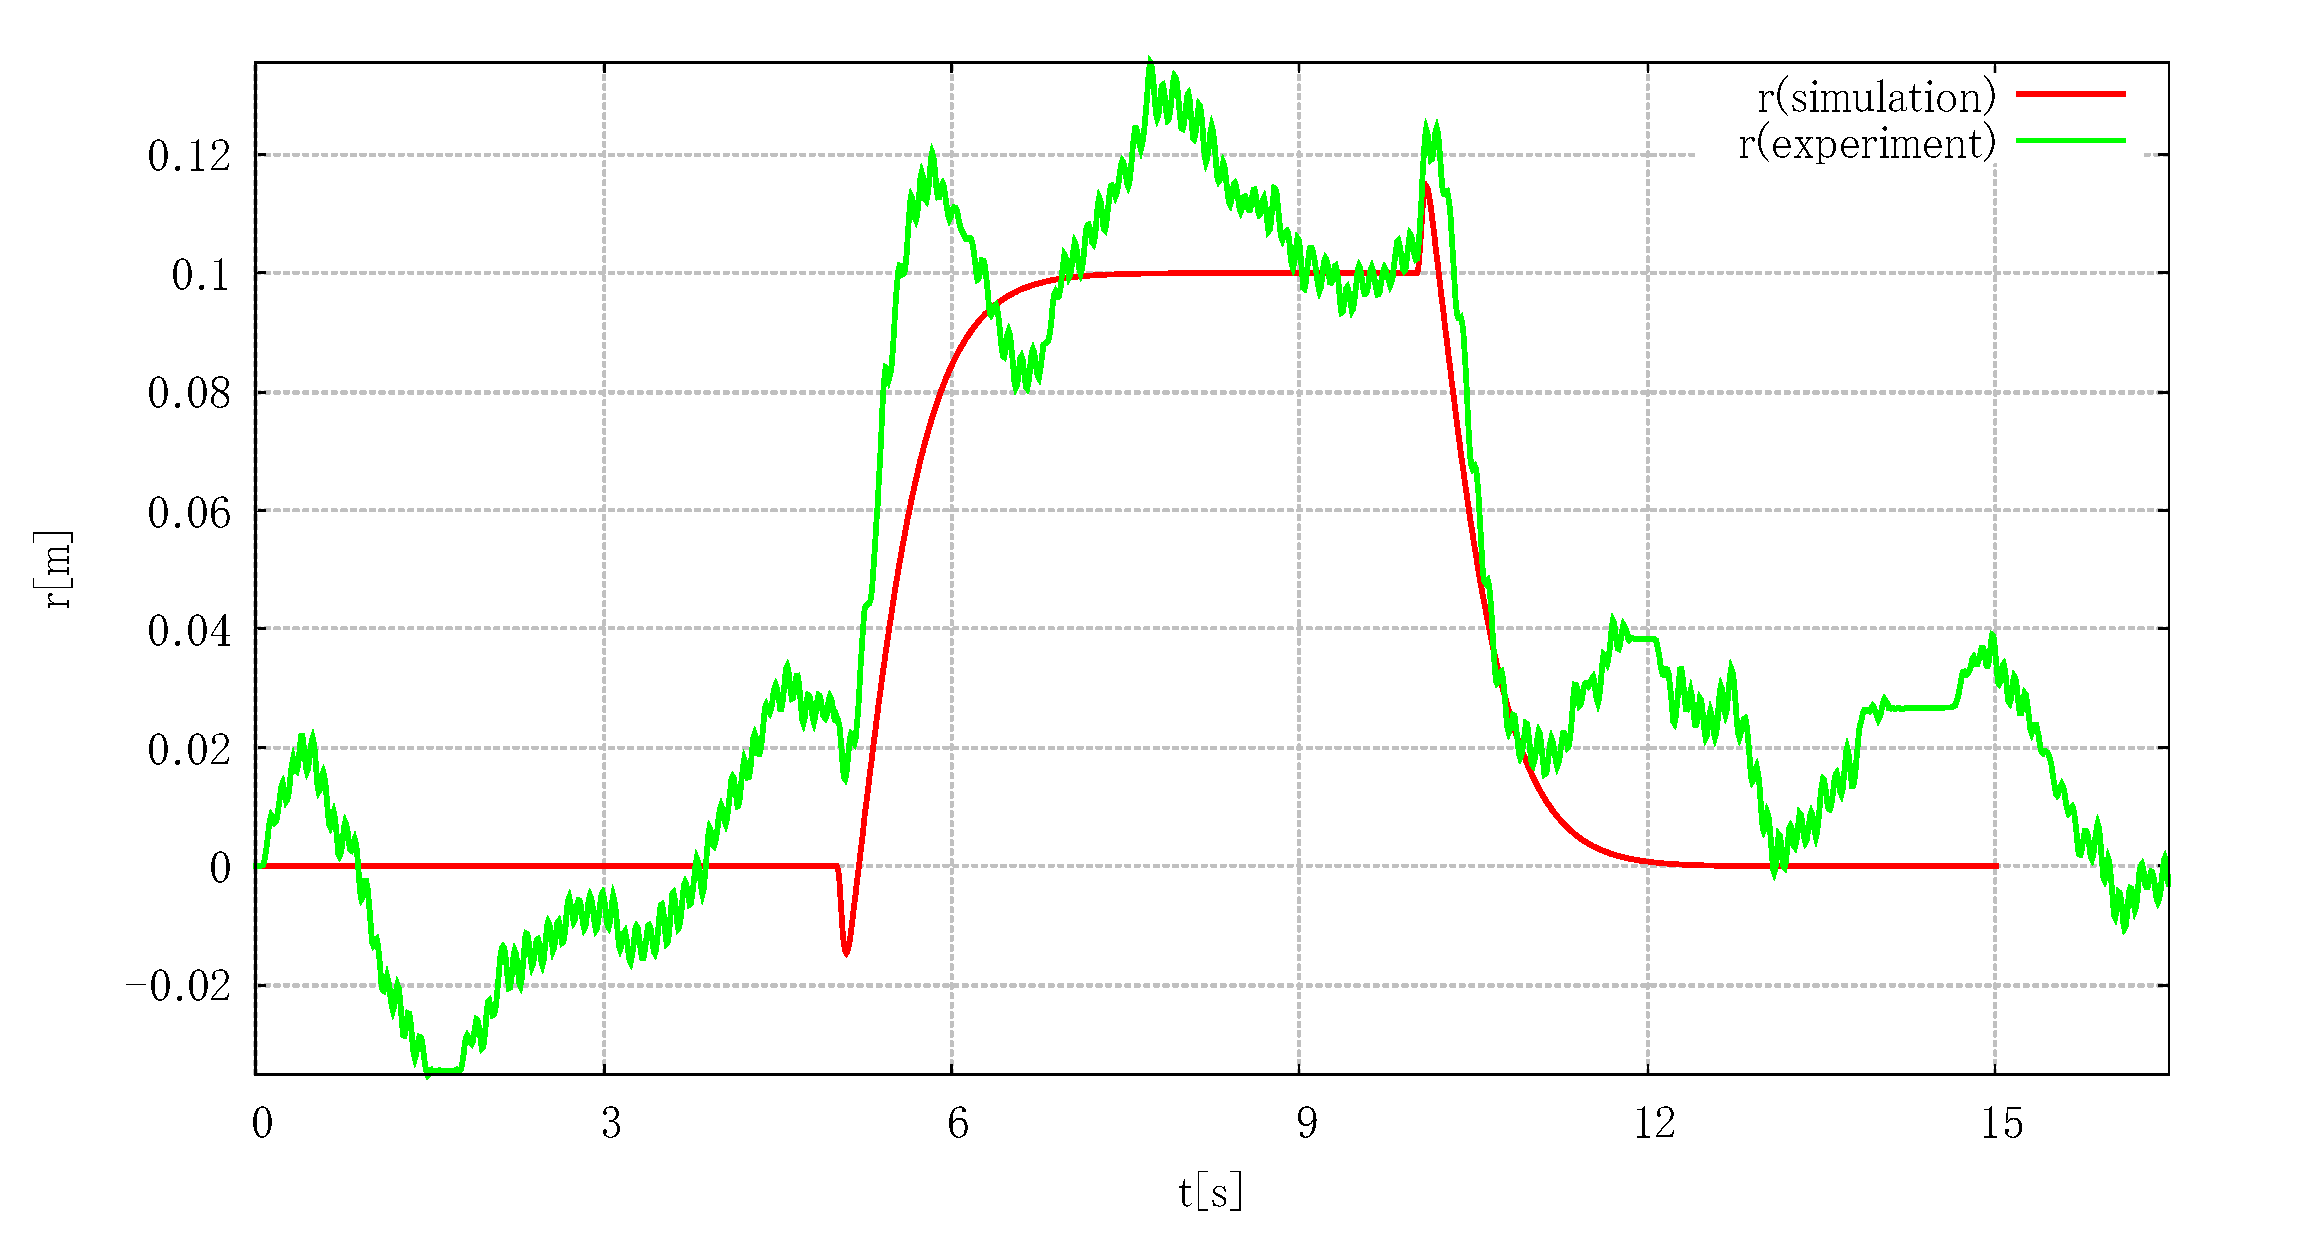
\includegraphics[width=0.49\linewidth]{gazo/experiment_Q55obs30dt10R.eps}
		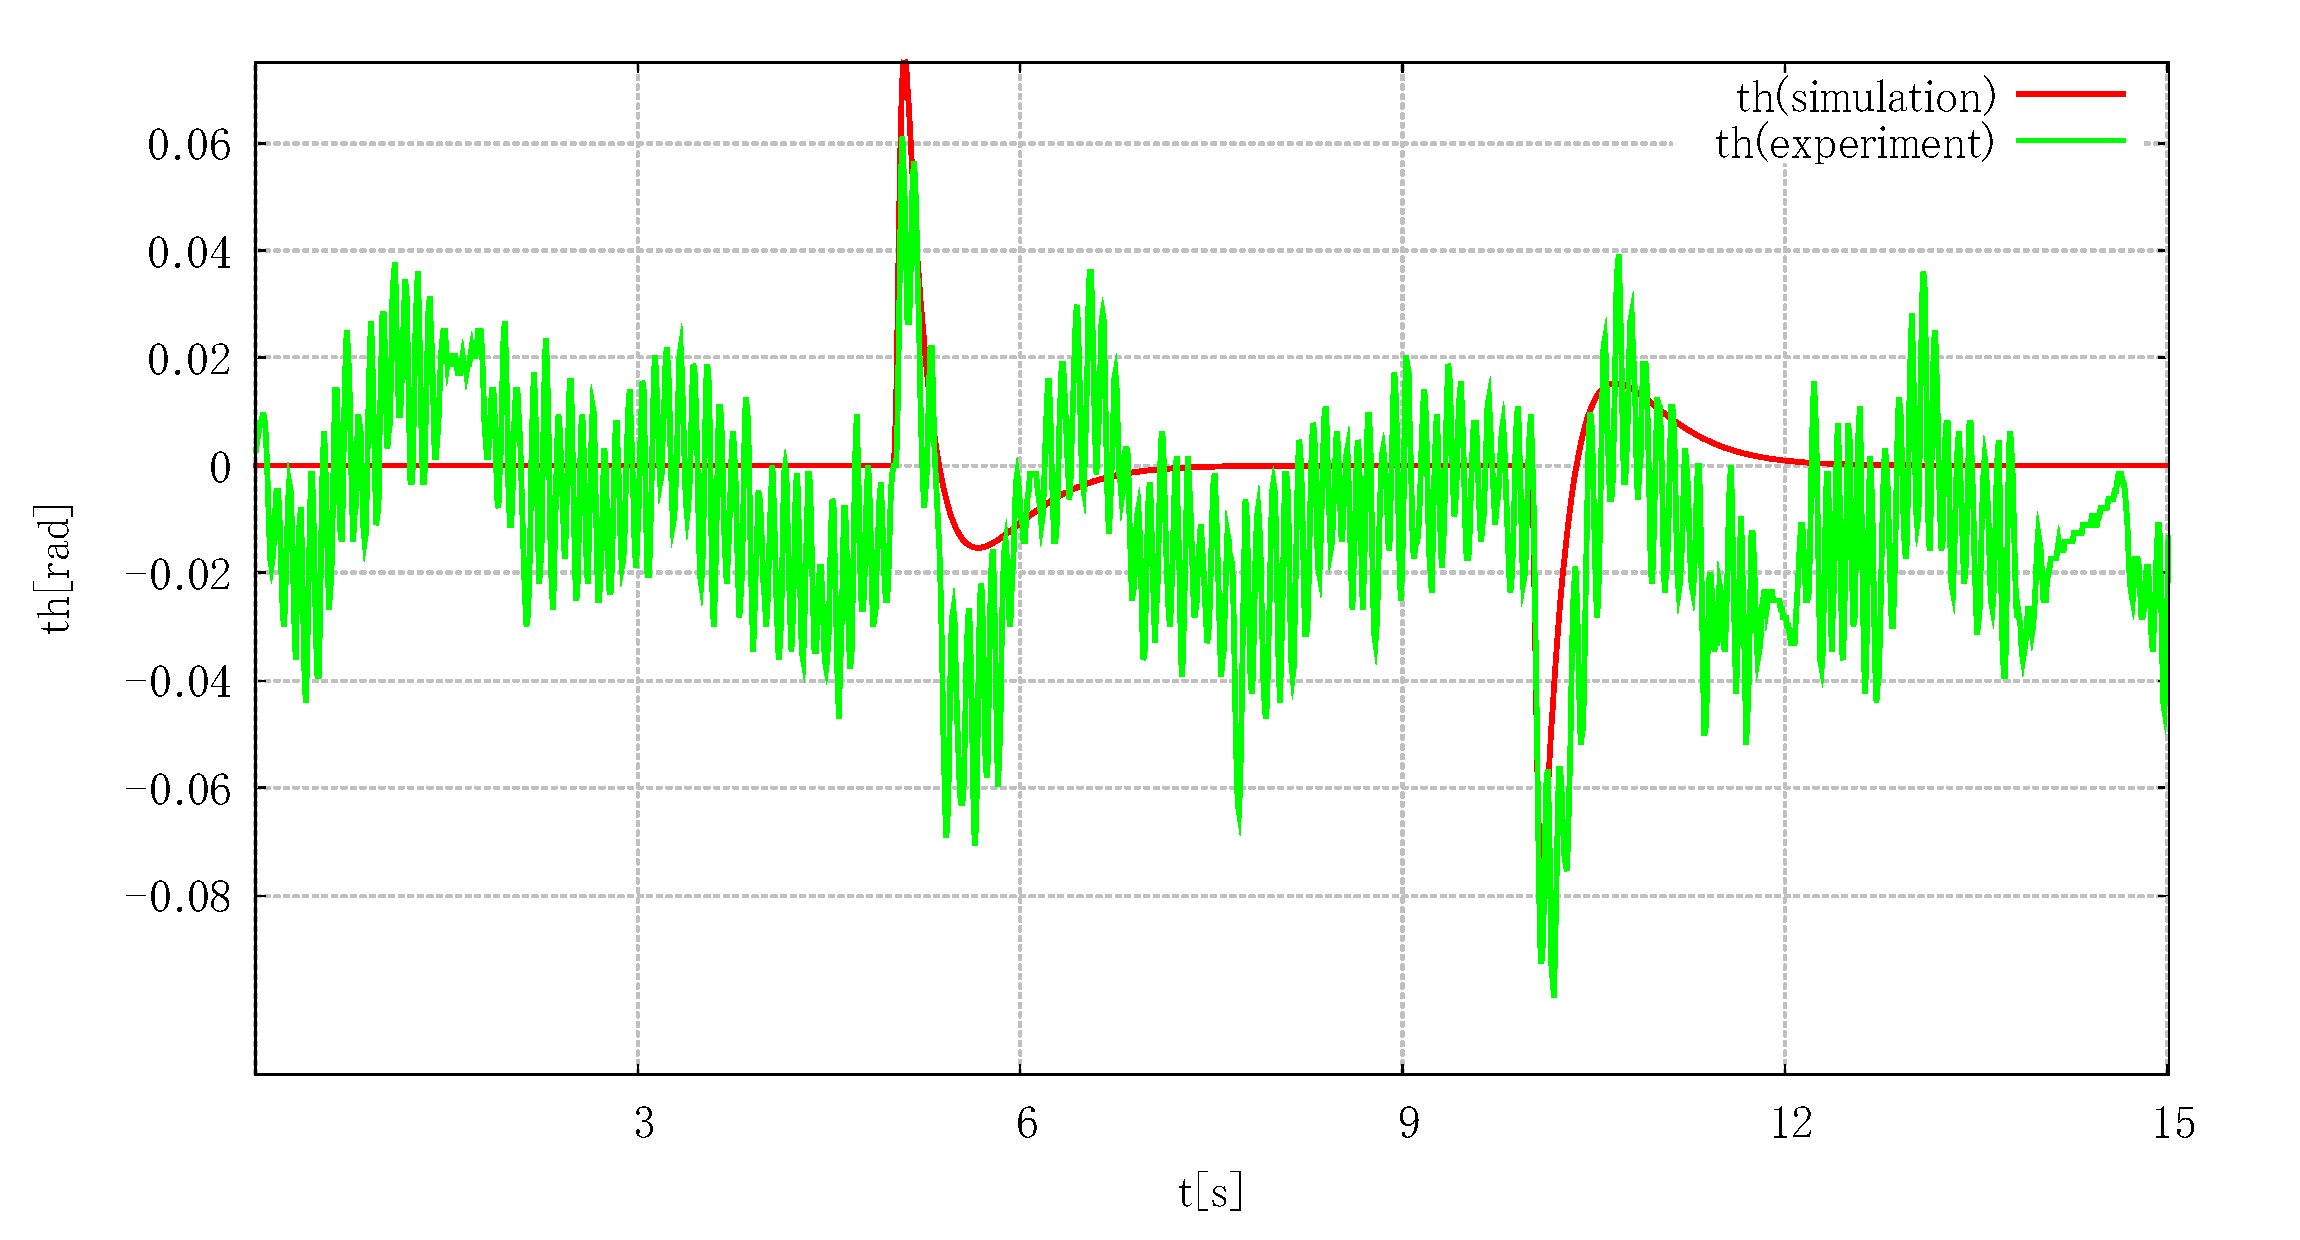
\includegraphics[width=0.49\linewidth]{gazo/experiment_Q55obs30dt10TH.eps}
		\caption{比較結果その7(左図がr,右図が$\theta$)}
		\label{image:sono7}
	\end{figure}
	\begin{figure}[H]
		\centering
		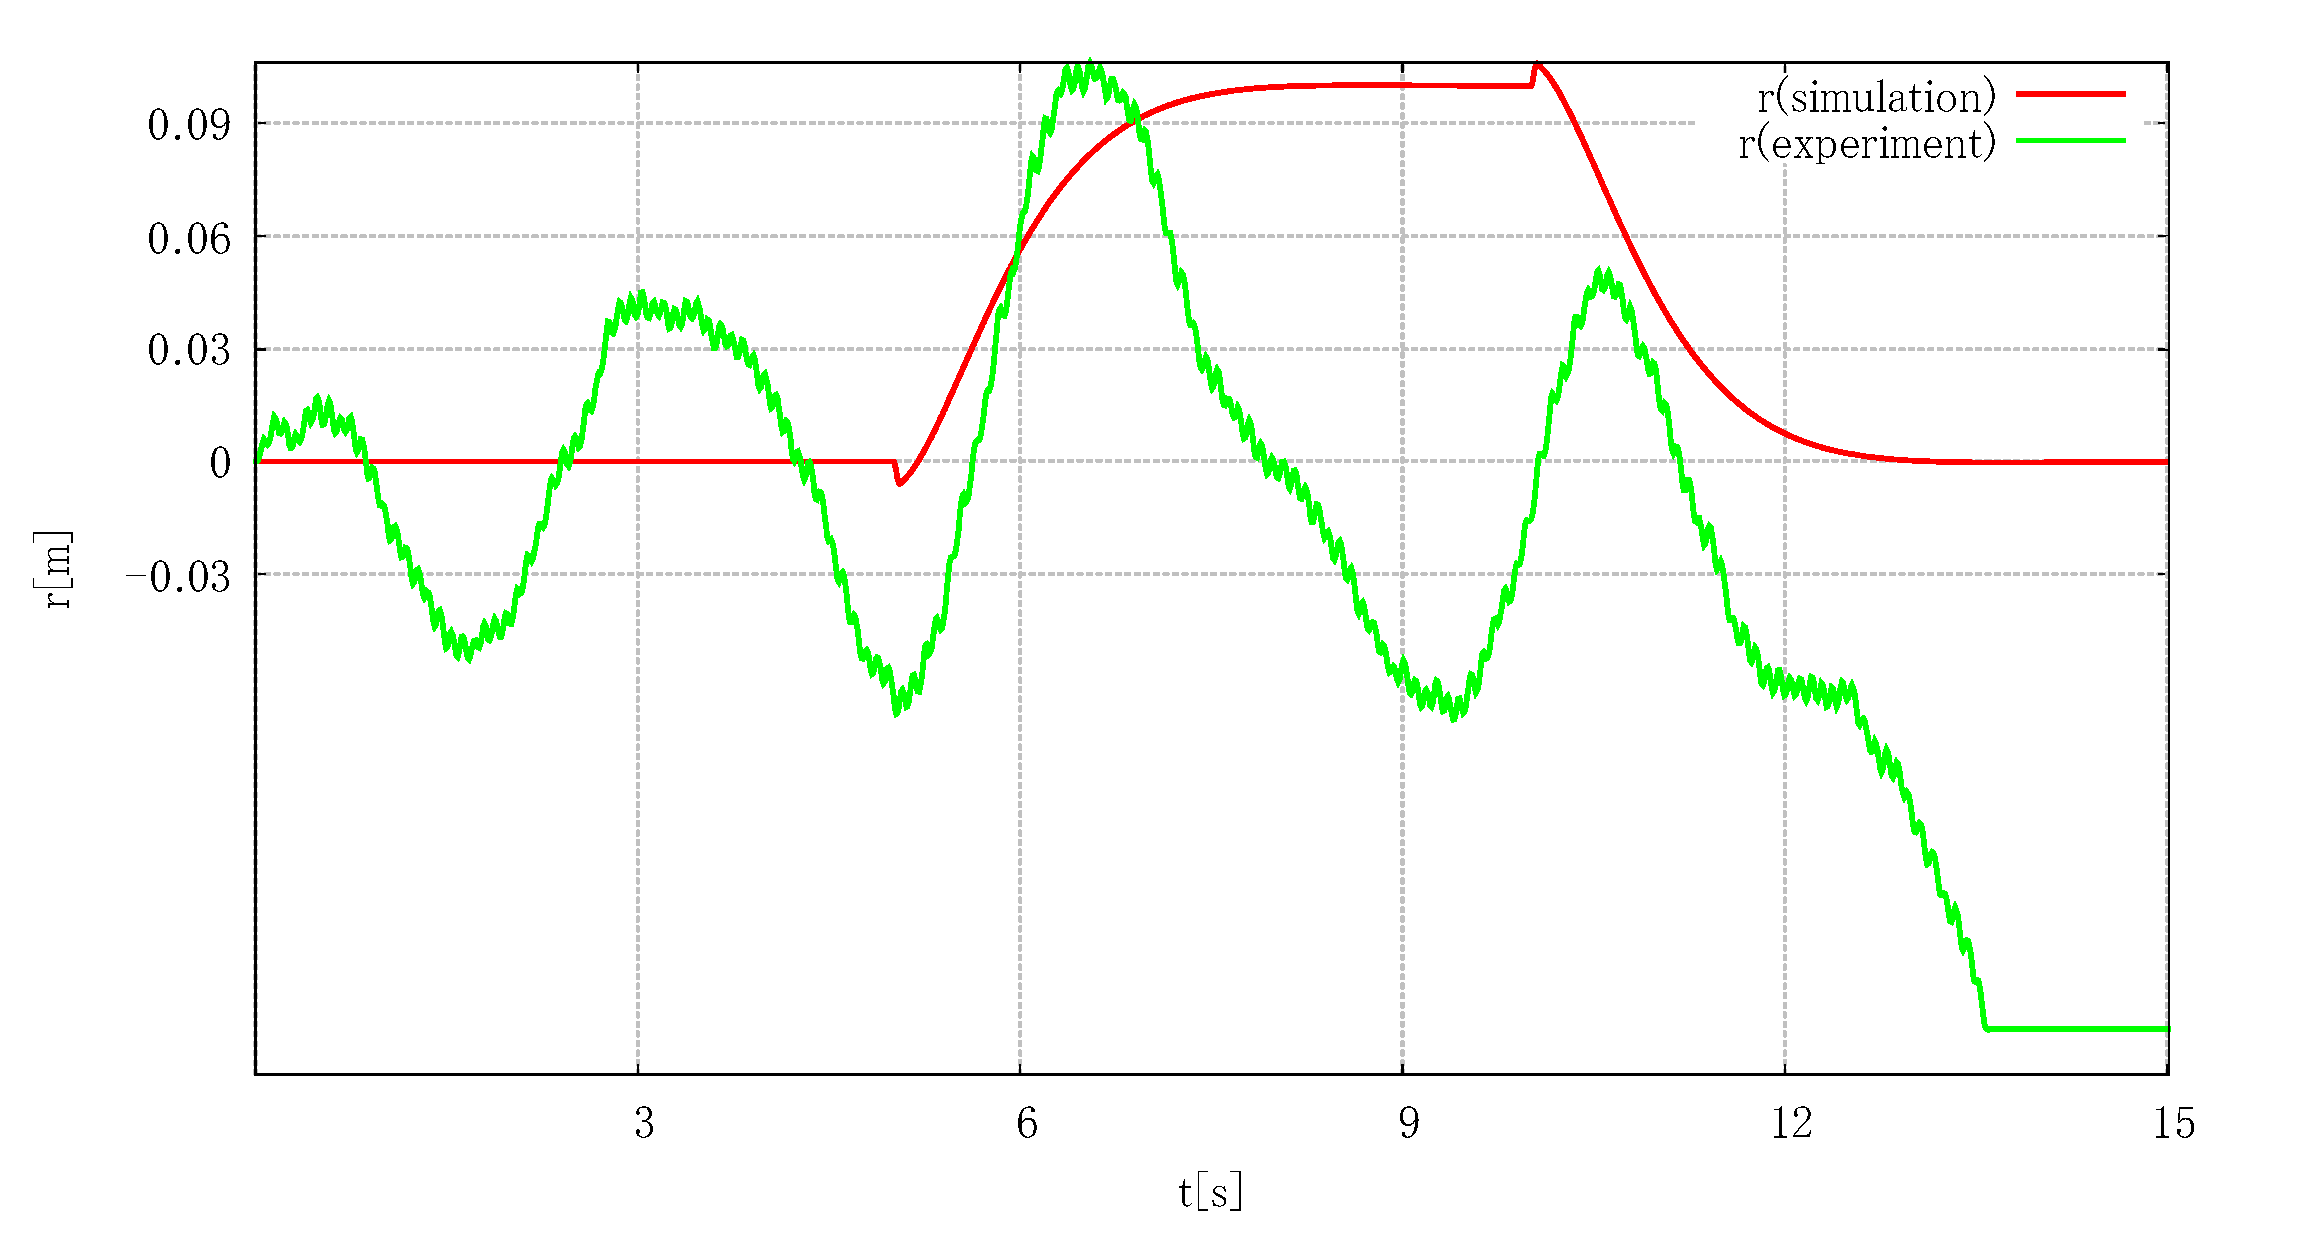
\includegraphics[width=0.49\linewidth]{gazo/experiment_Q56obs30dt10R.eps}
		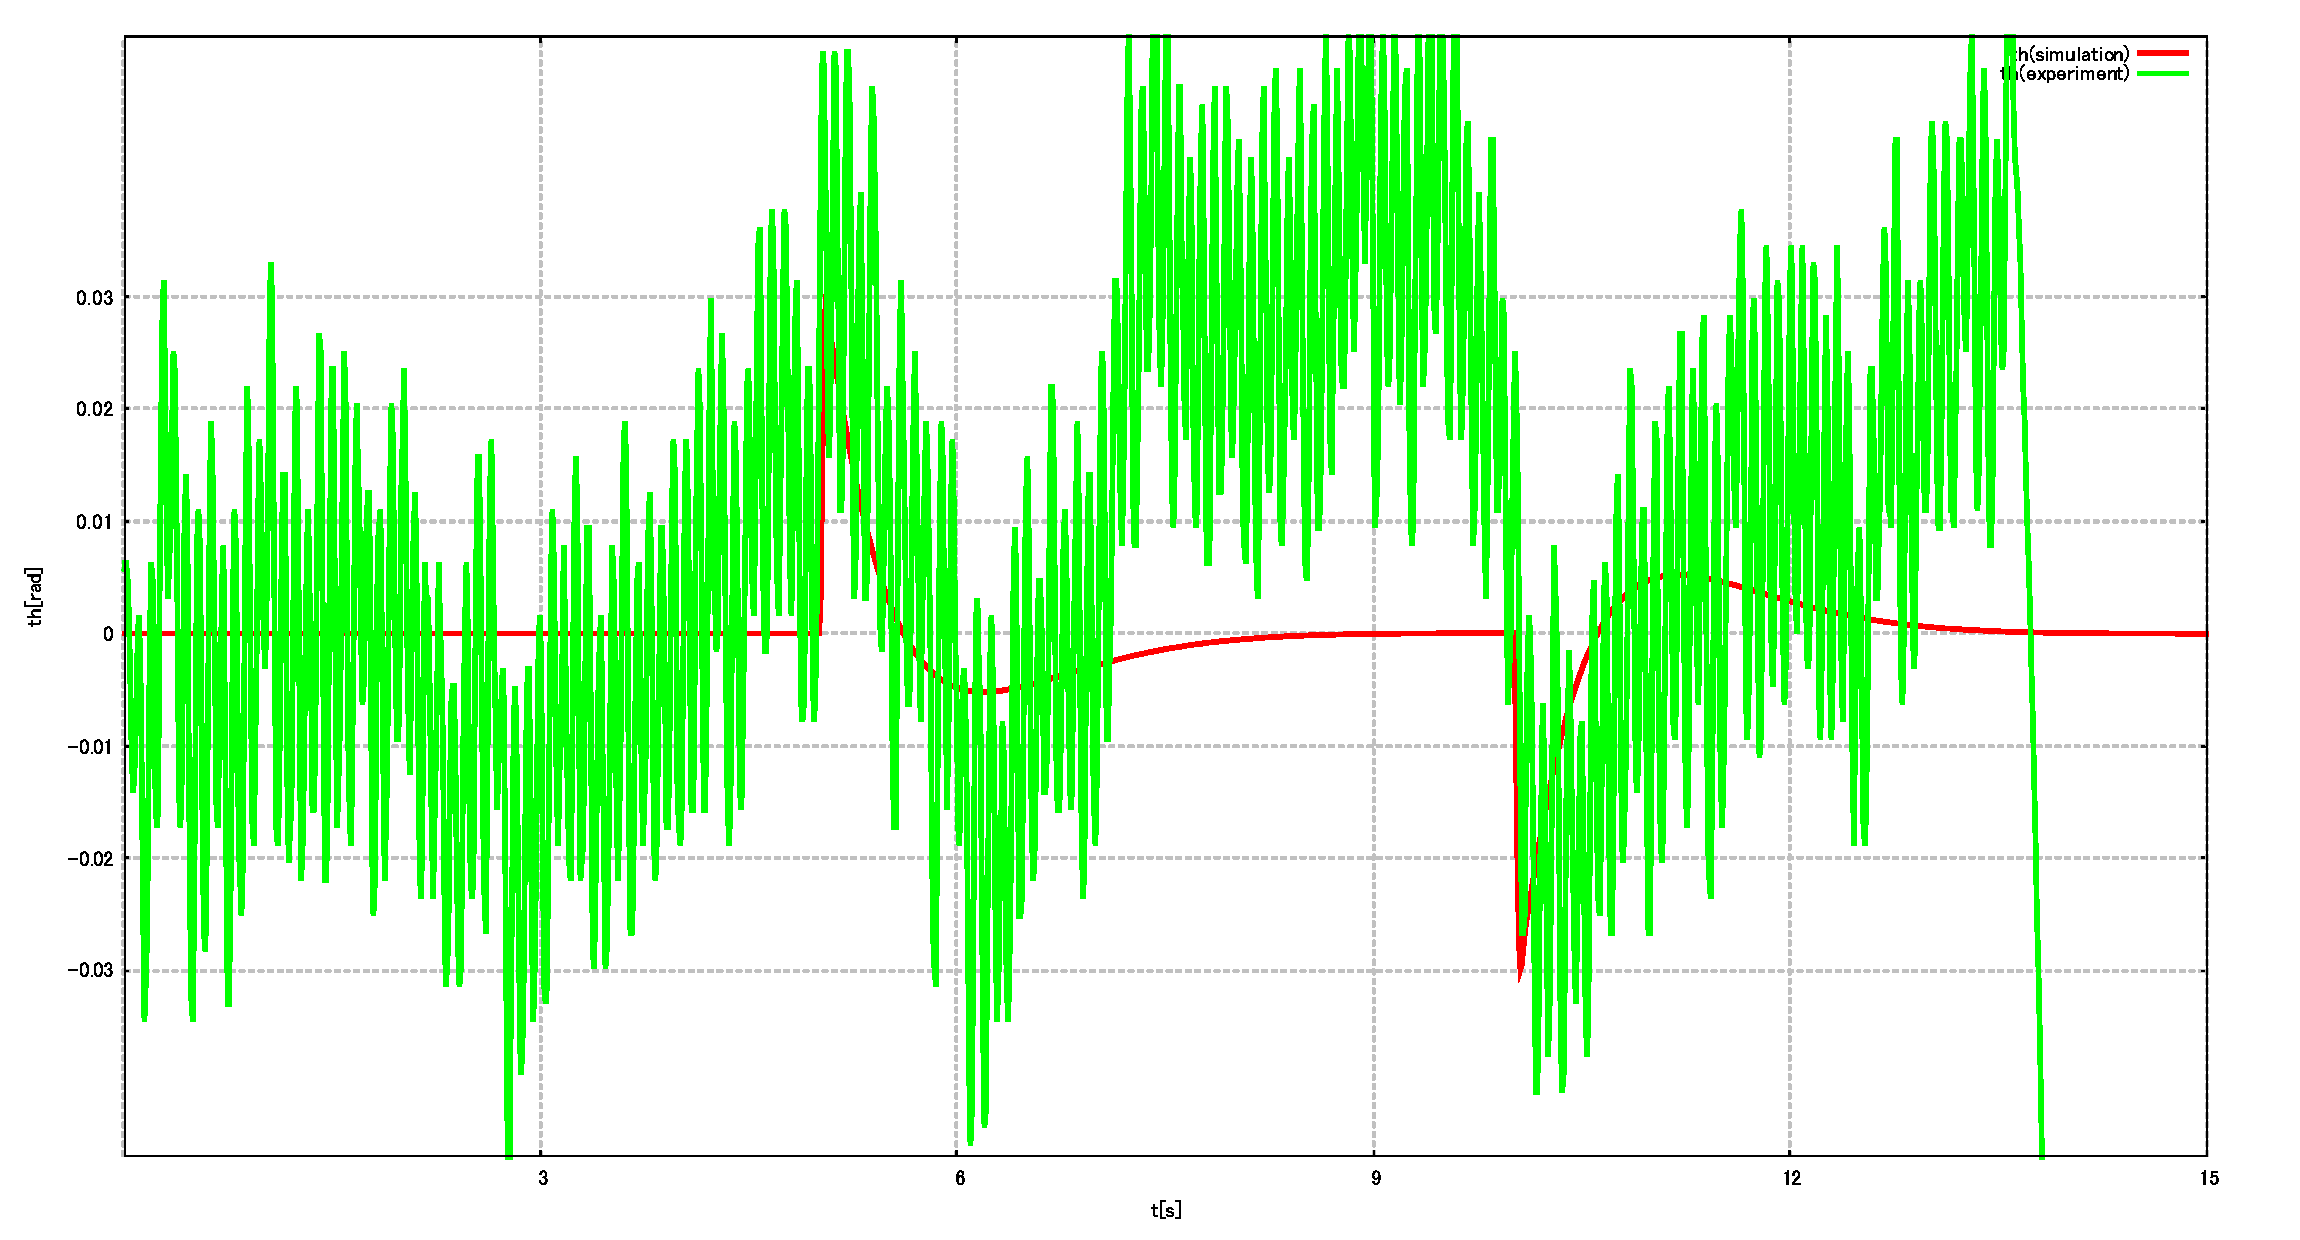
\includegraphics[width=0.49\linewidth]{gazo/experiment_Q56obs30dt10TH.eps}
		\caption{比較結果その8(左図がr,右図が$\theta$)}
		\label{image:sono8}
	\end{figure}
	\begin{figure}[H]
		\centering
		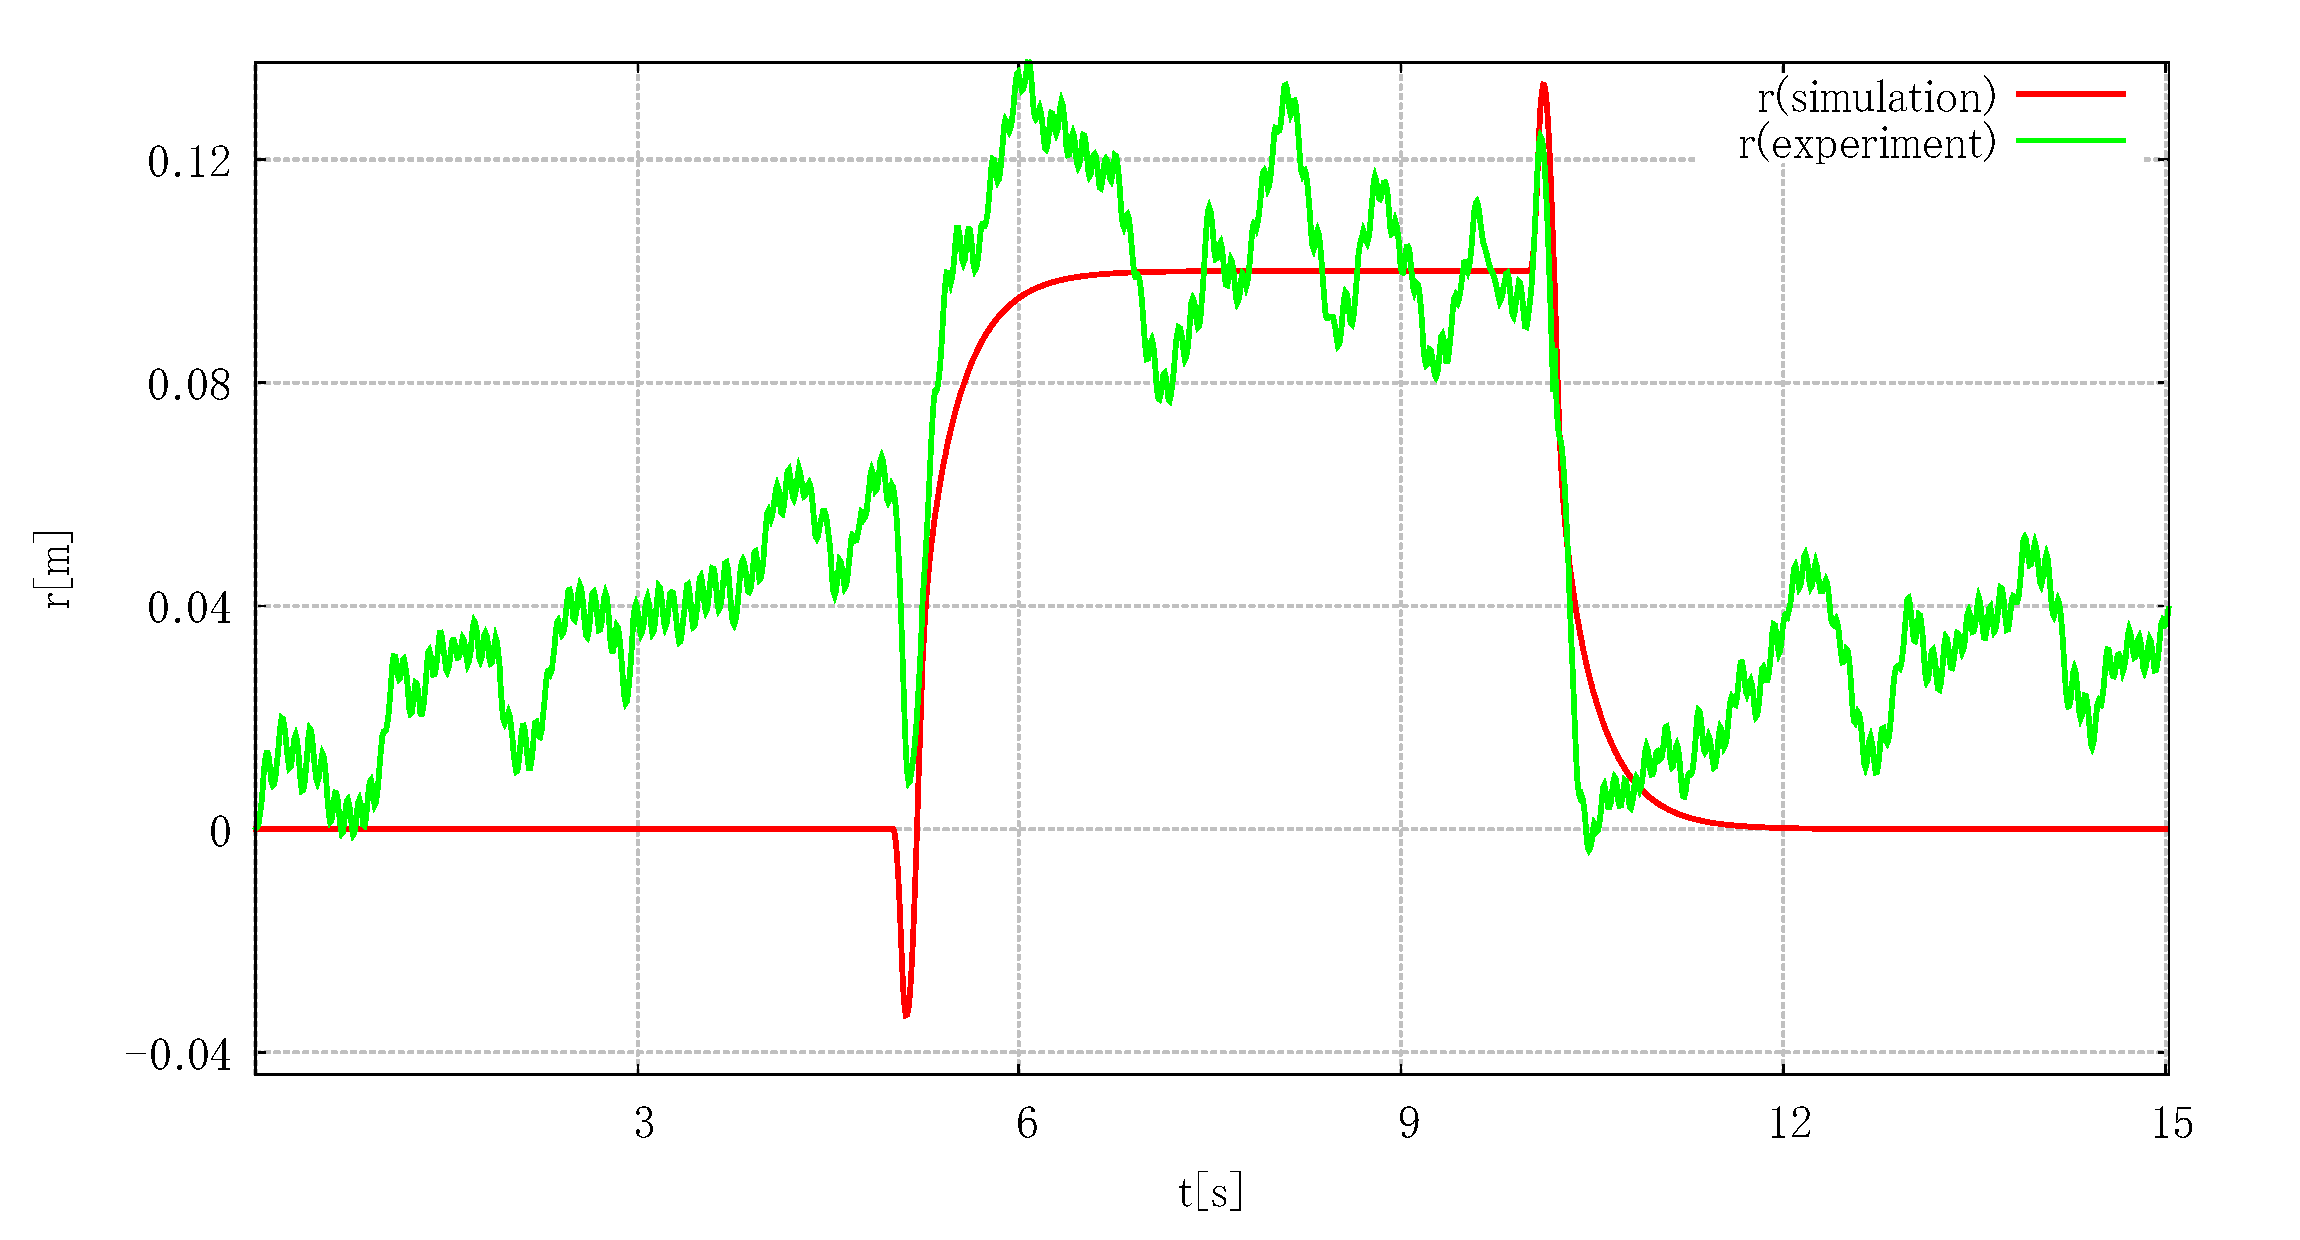
\includegraphics[width=0.49\linewidth]{gazo/experiment_Q65obs30dt10R.eps}
		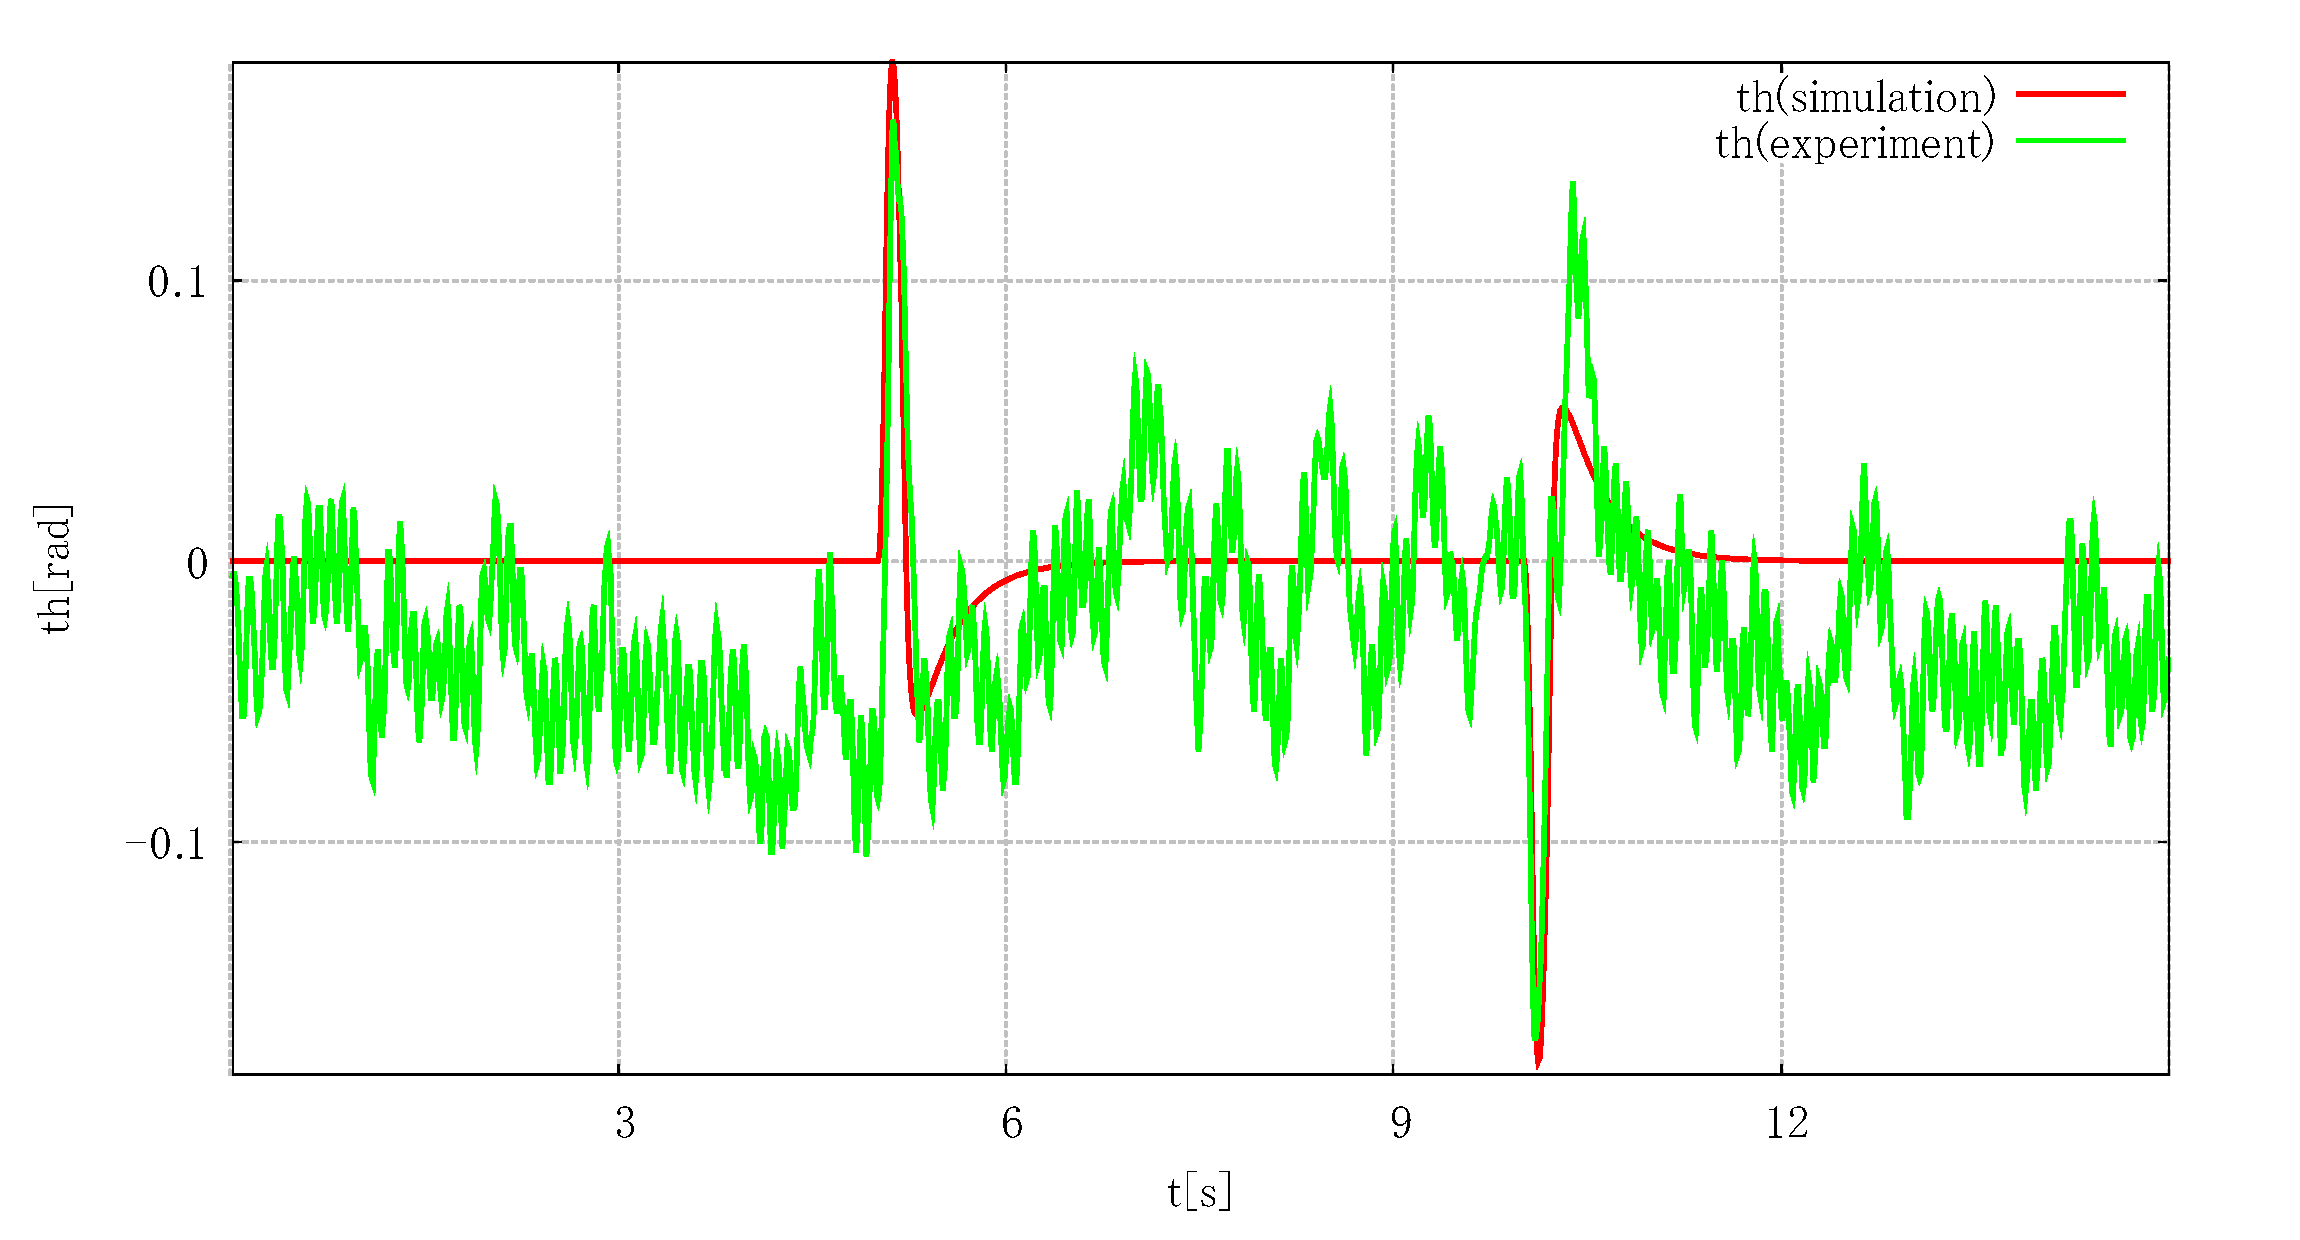
\includegraphics[width=0.49\linewidth]{gazo/experiment_Q65obs30dt10TH.eps}
		\caption{比較結果その9(左図がr,右図が$\theta$)}
		\label{image:sono9}
	\end{figure}
	\begin{figure}[H]
		\centering
		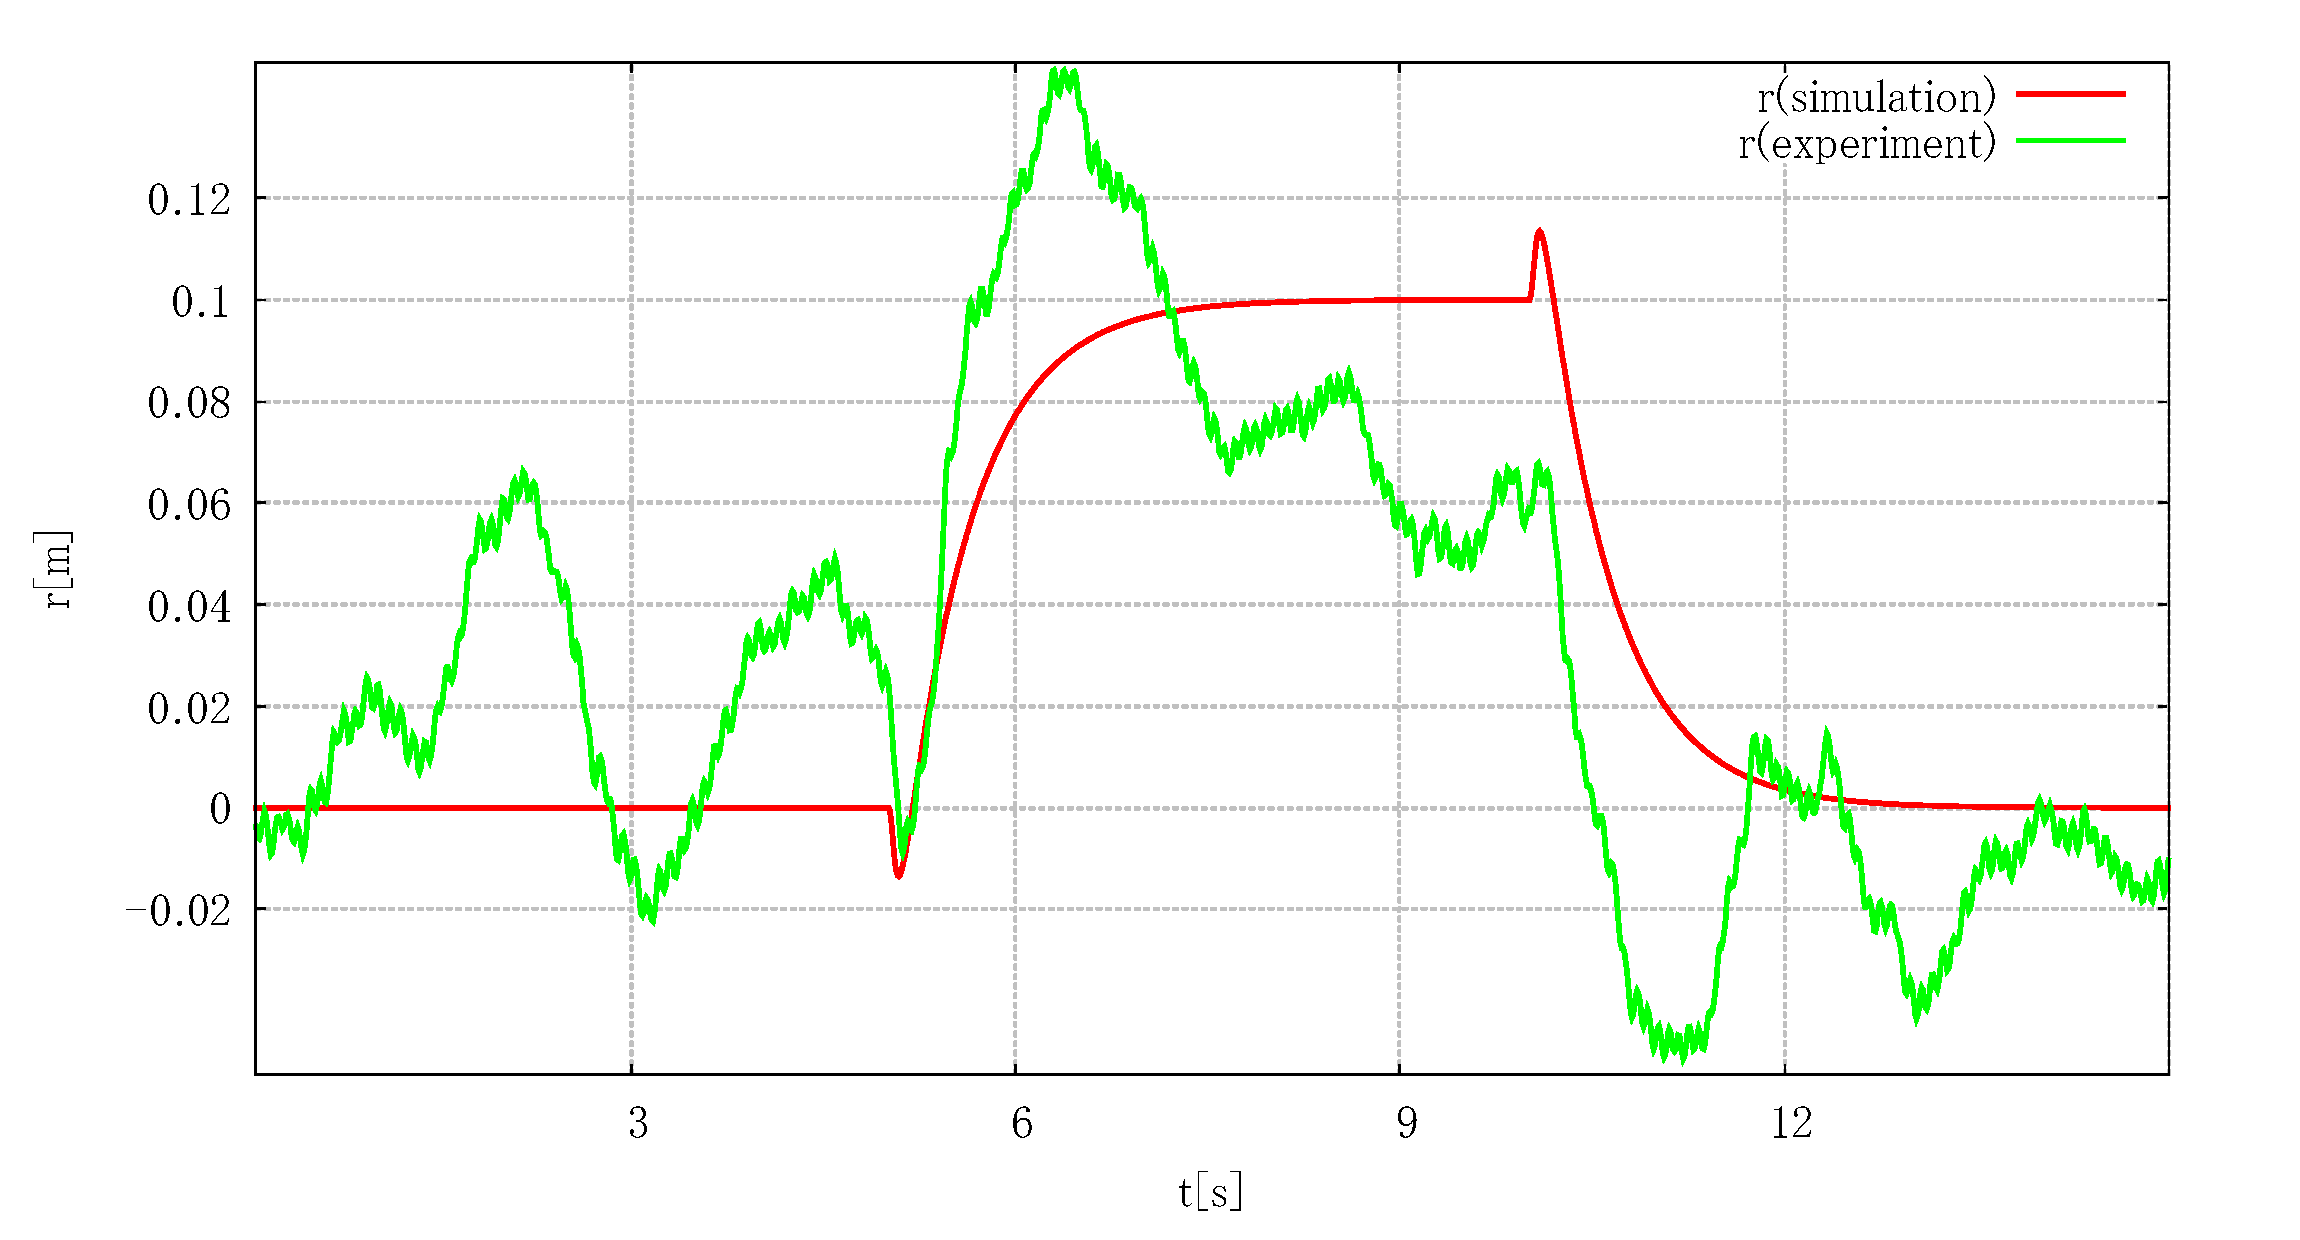
\includegraphics[width=0.49\linewidth]{gazo/experiment_Q55obs60dt10R.eps}
		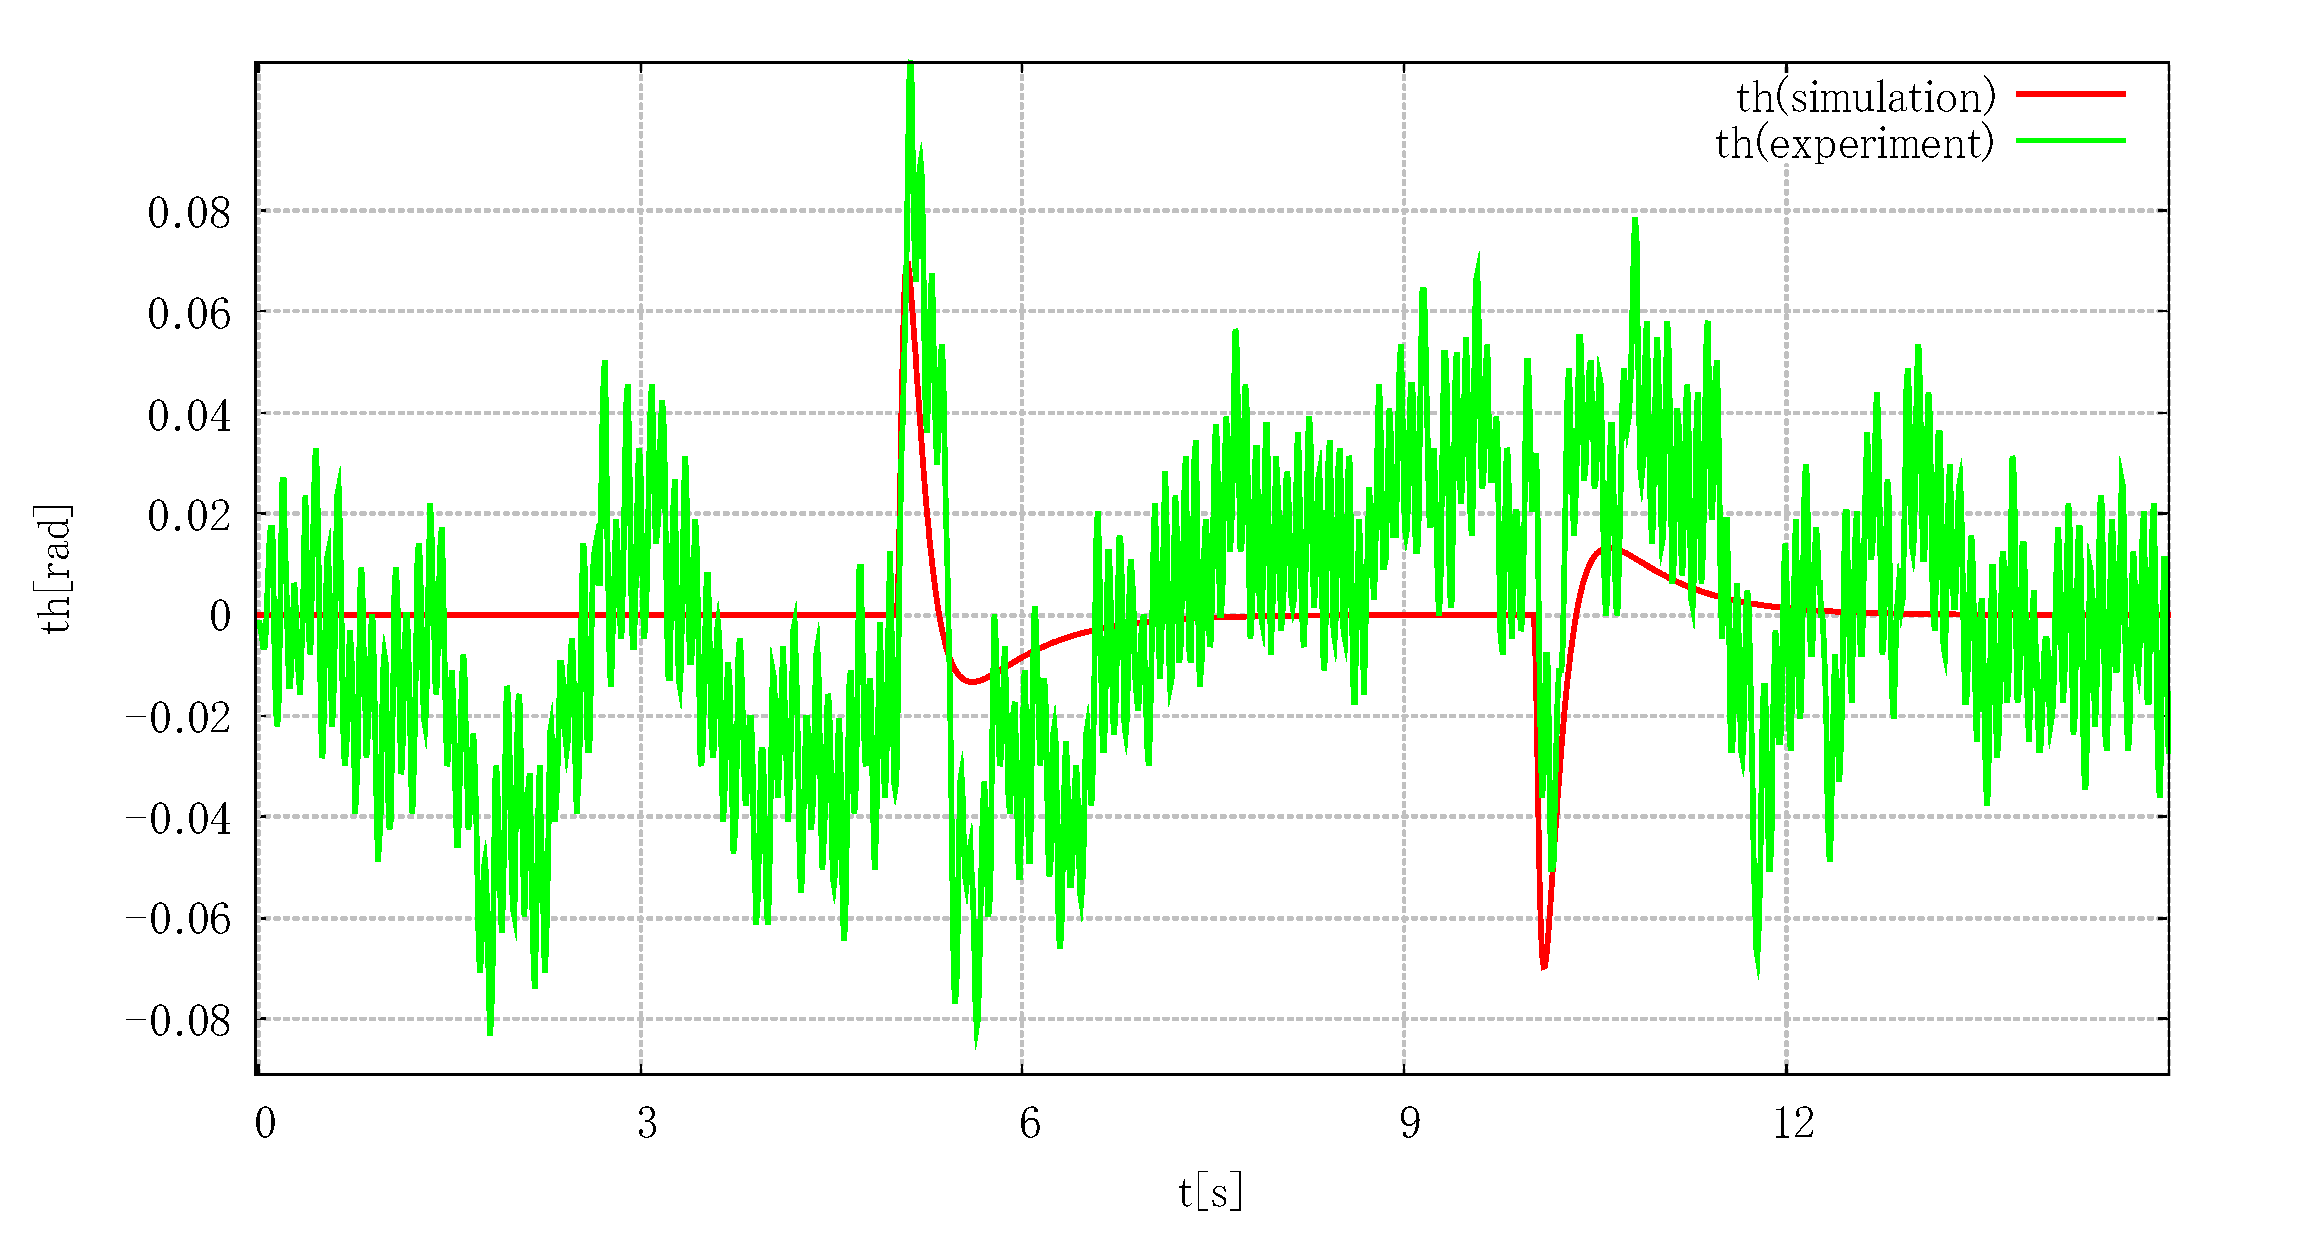
\includegraphics[width=0.49\linewidth]{gazo/experiment_Q55obs60dt10TH.eps}
		\caption{比較結果その10(左図がr,右図が$\theta$)}
		\label{image:sono10}
	\end{figure}
	\begin{figure}[H]
		\centering
		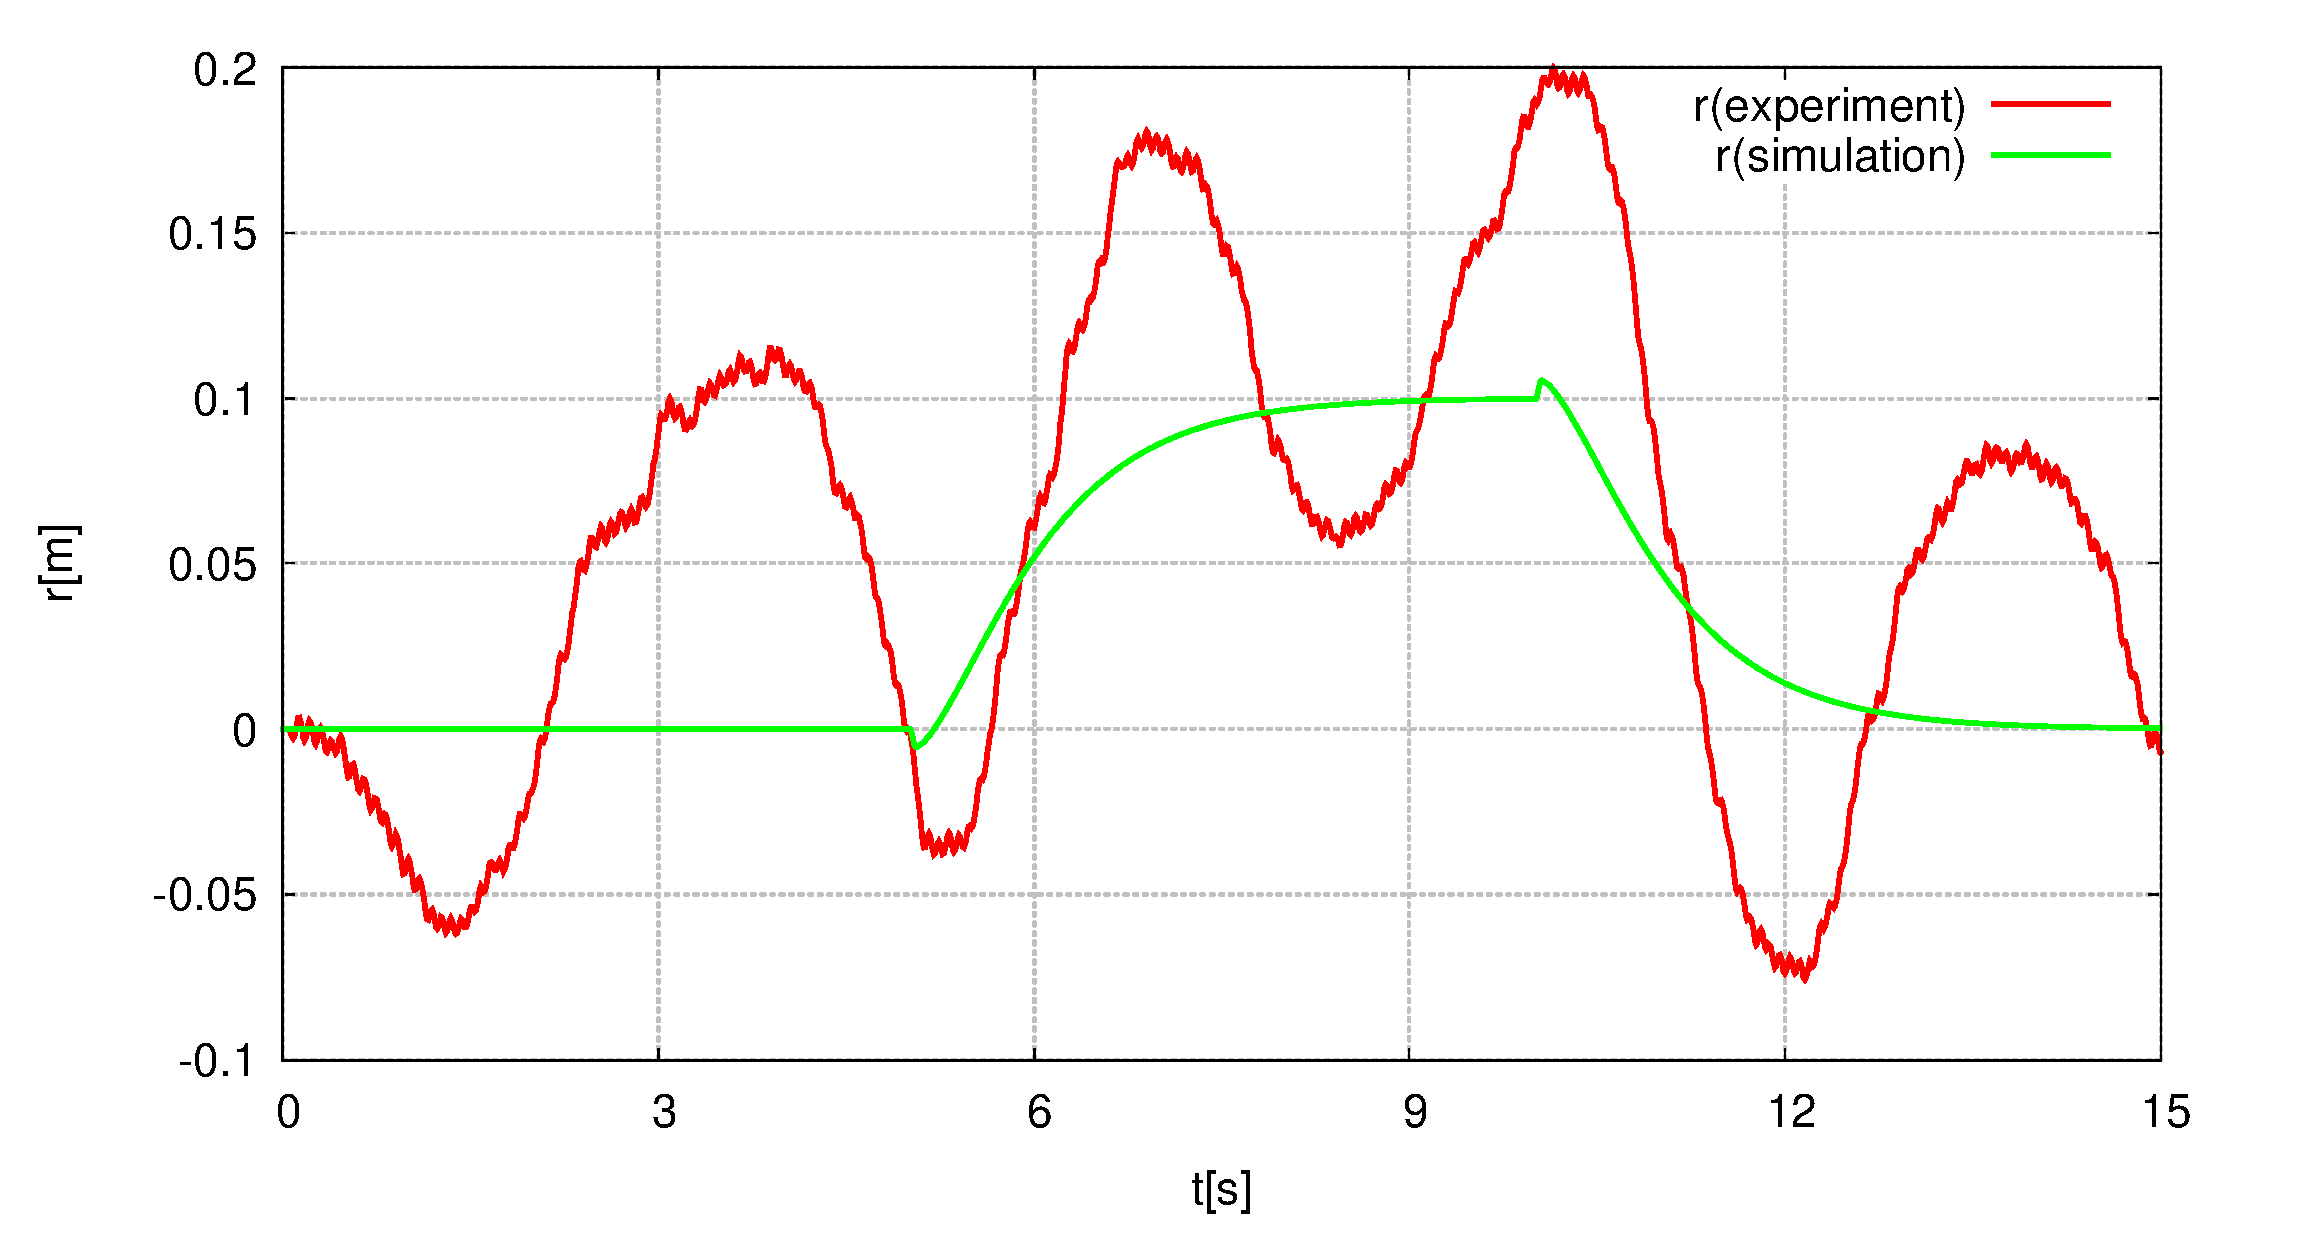
\includegraphics[width=0.49\linewidth]{gazo/experiment_Q56obs60dt10R2.eps}
		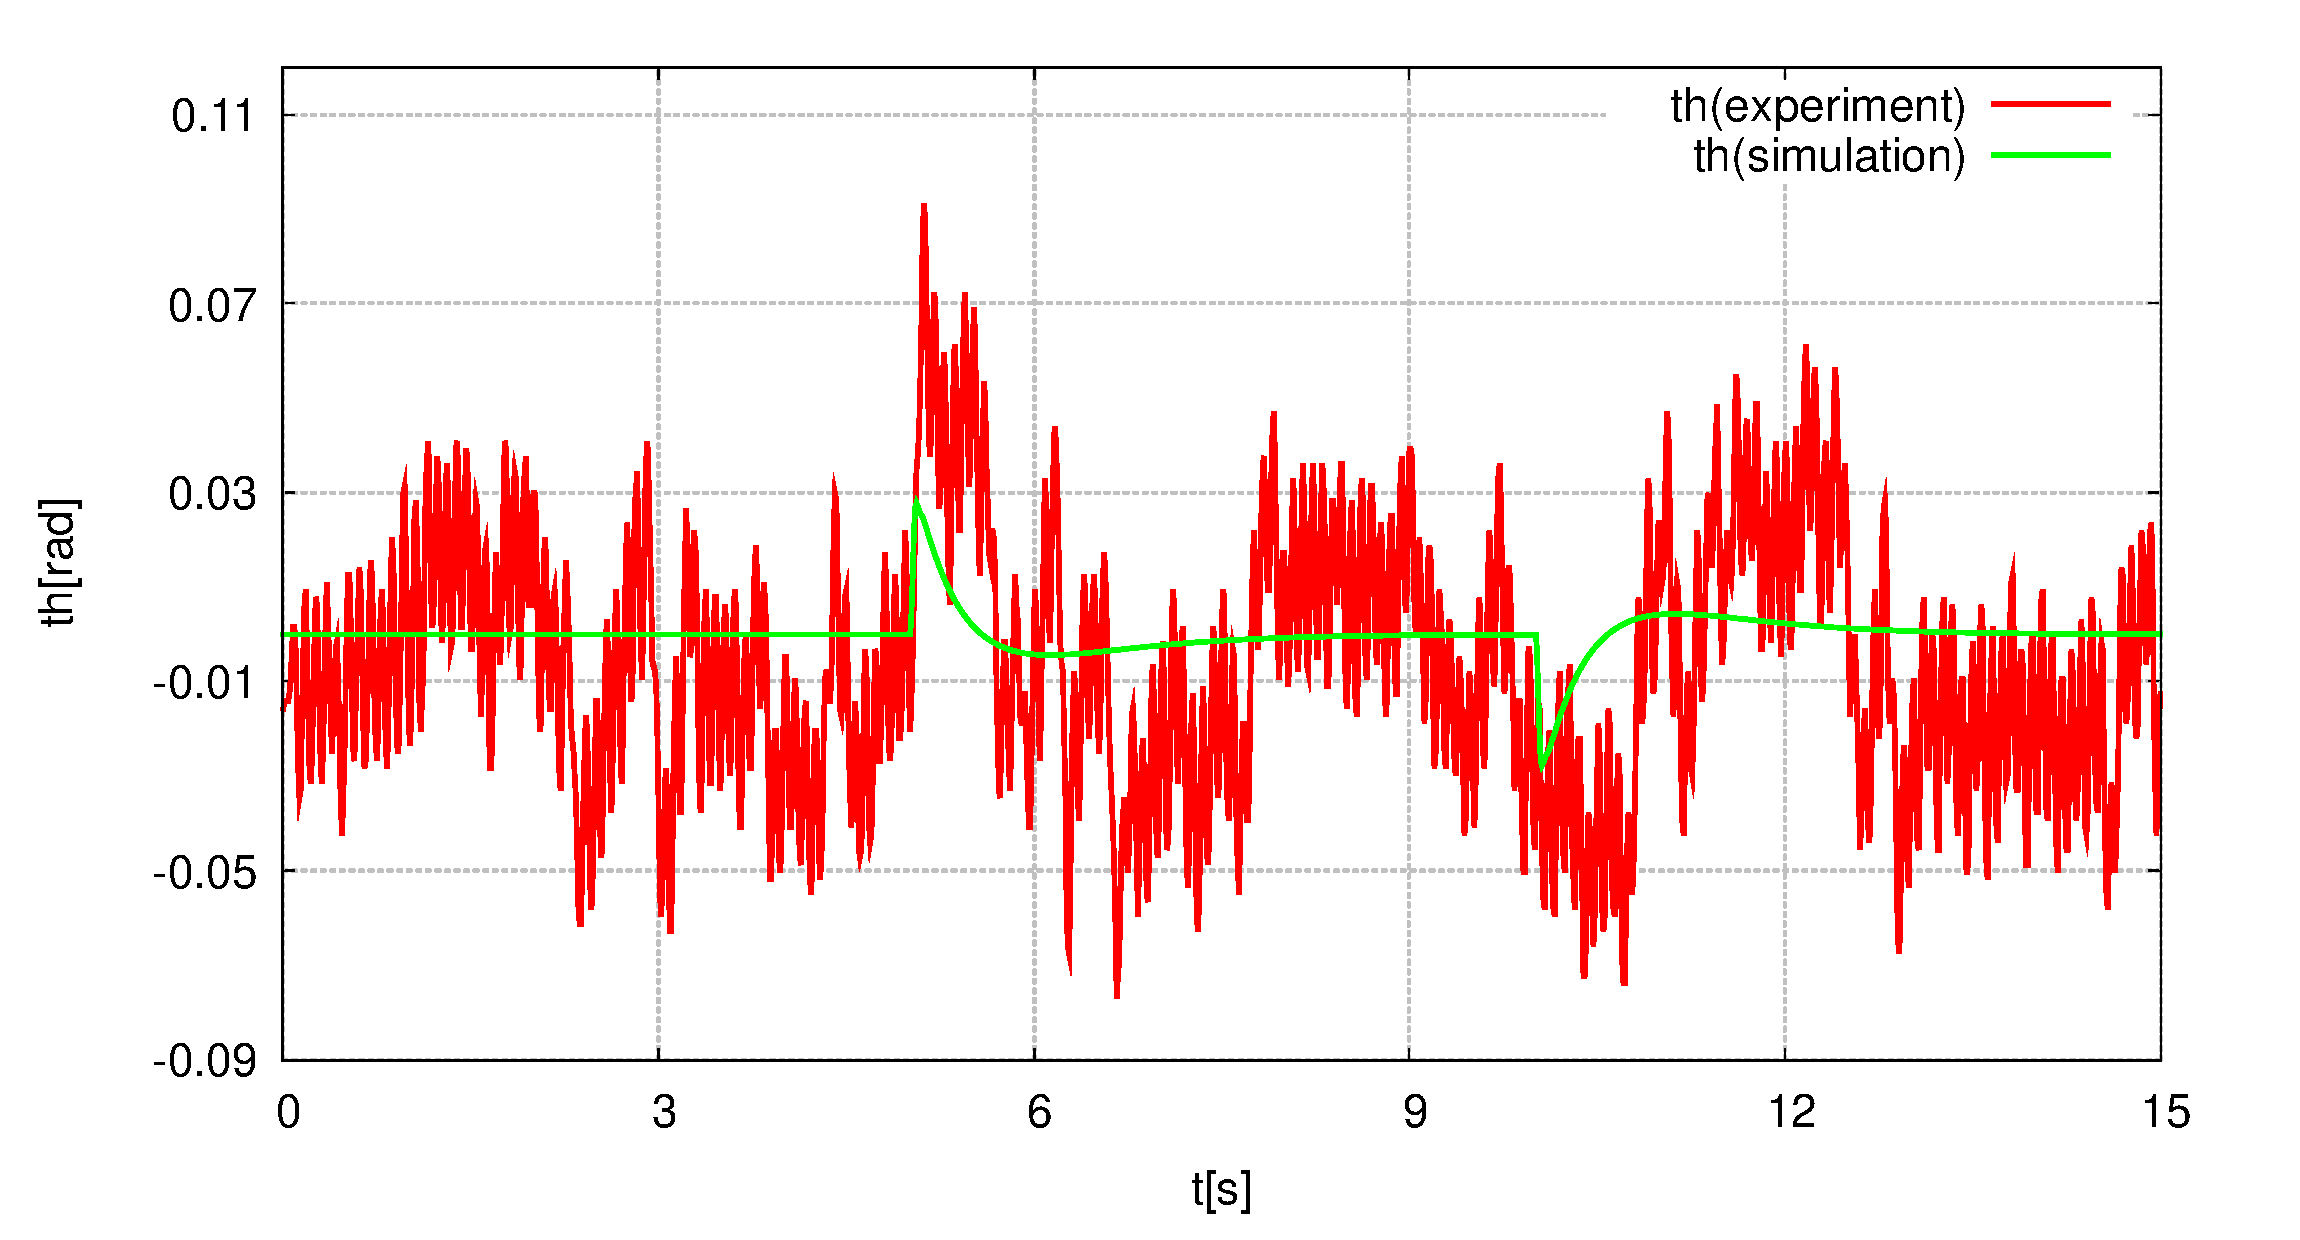
\includegraphics[width=0.49\linewidth]{gazo/experiment_Q56obs60dt10TH2.eps}
		\caption{比較結果その11(左図がr,右図が$\theta$)}
		\label{image:sono11}
	\end{figure}
	\begin{figure}[H]
		\centering
		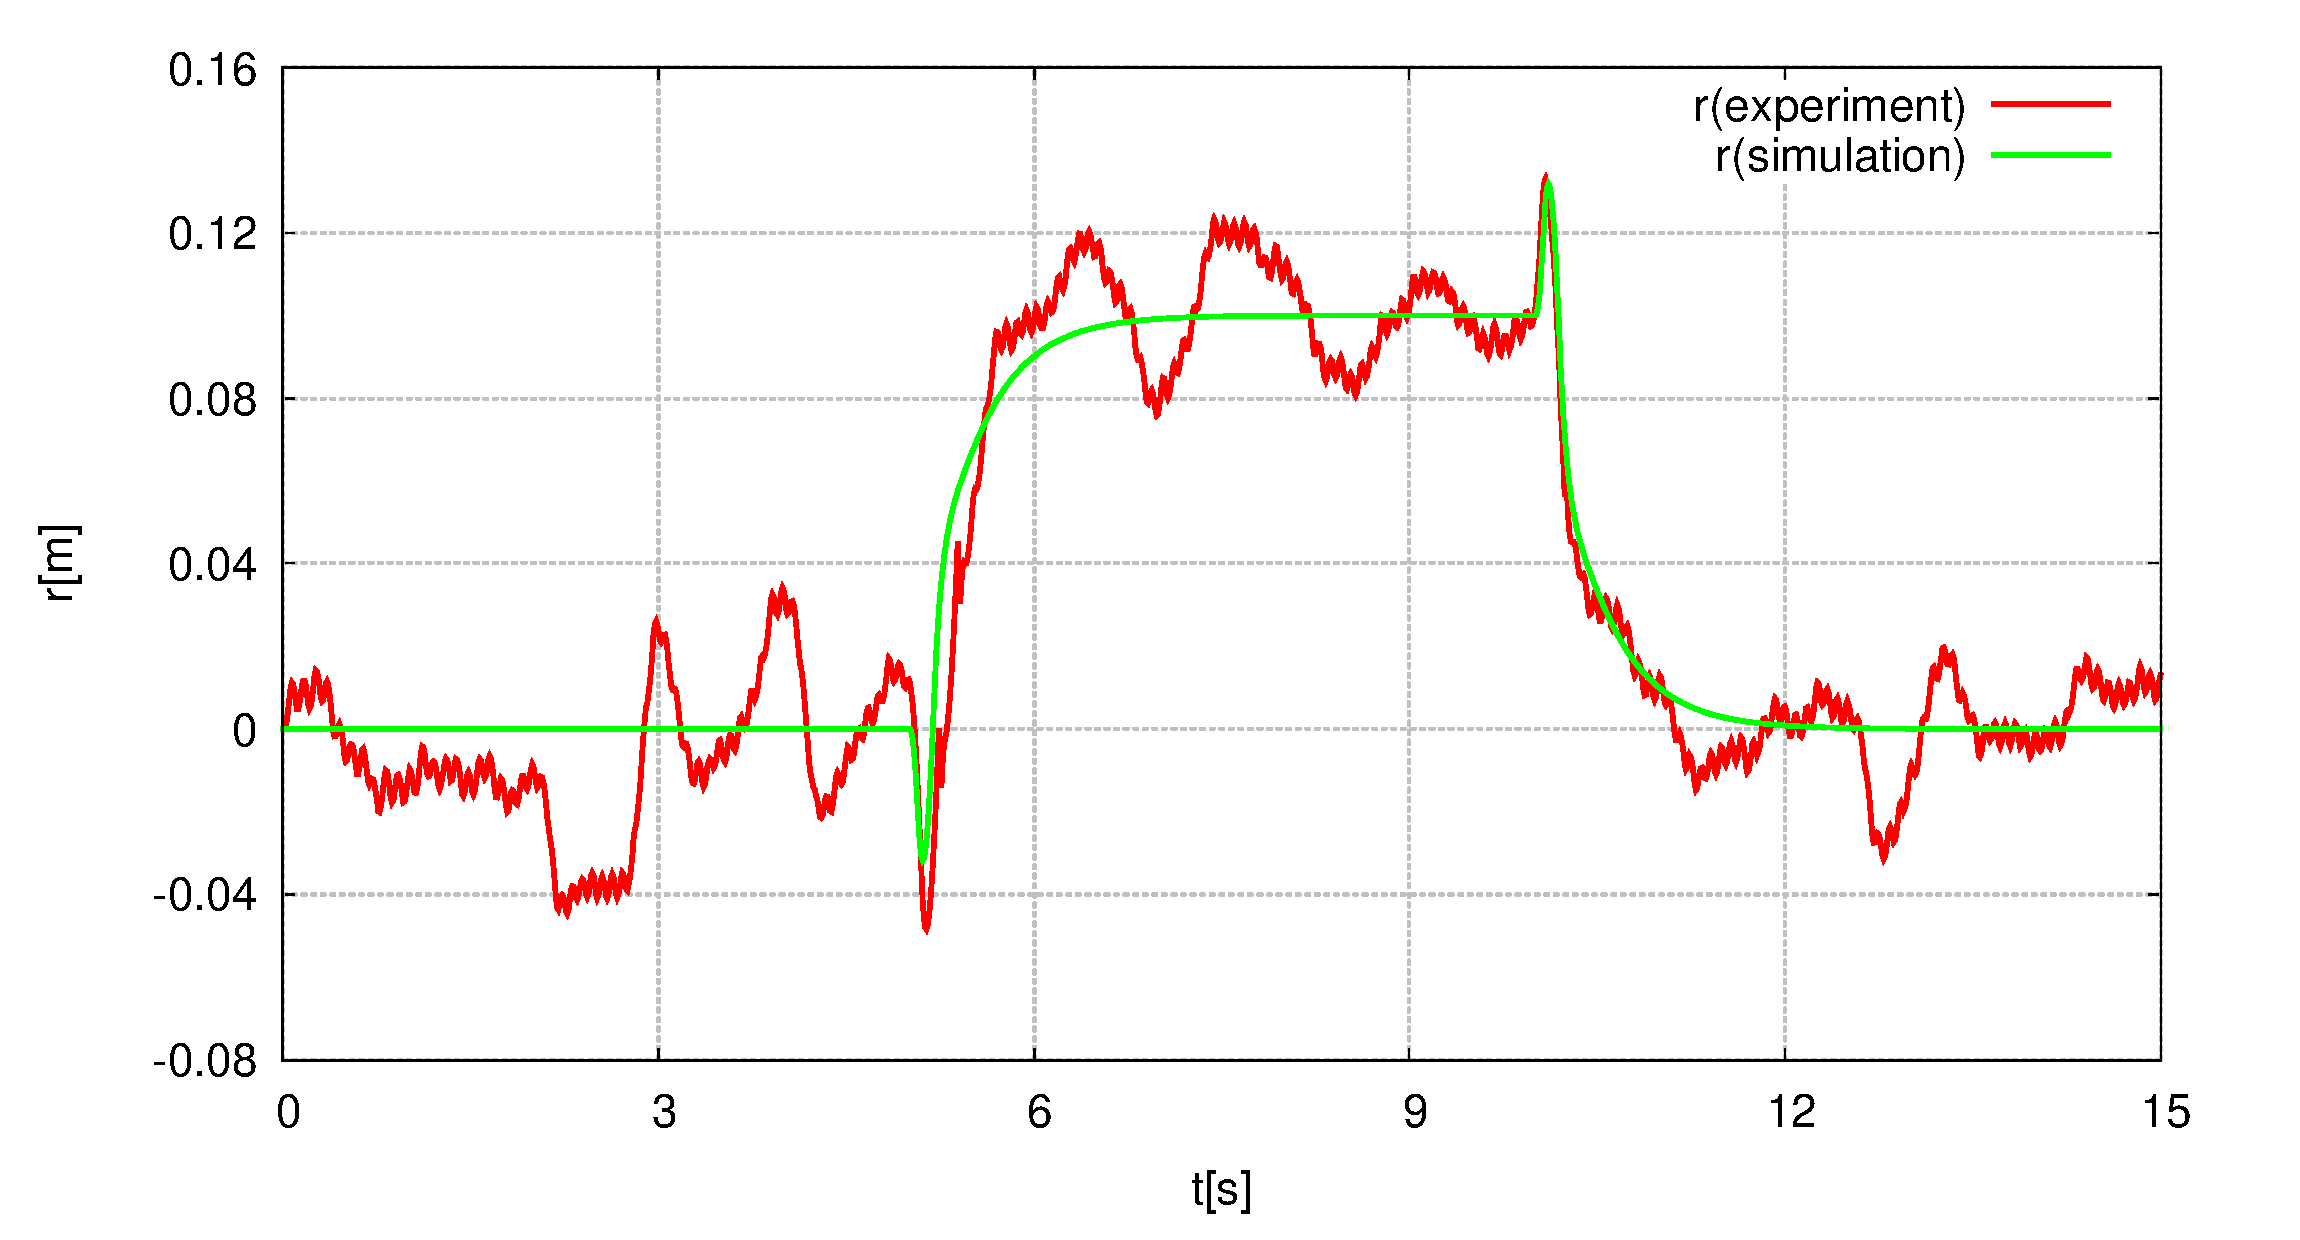
\includegraphics[width=0.49\linewidth]{gazo/experiment_Q65obs60dt10R2.eps}
		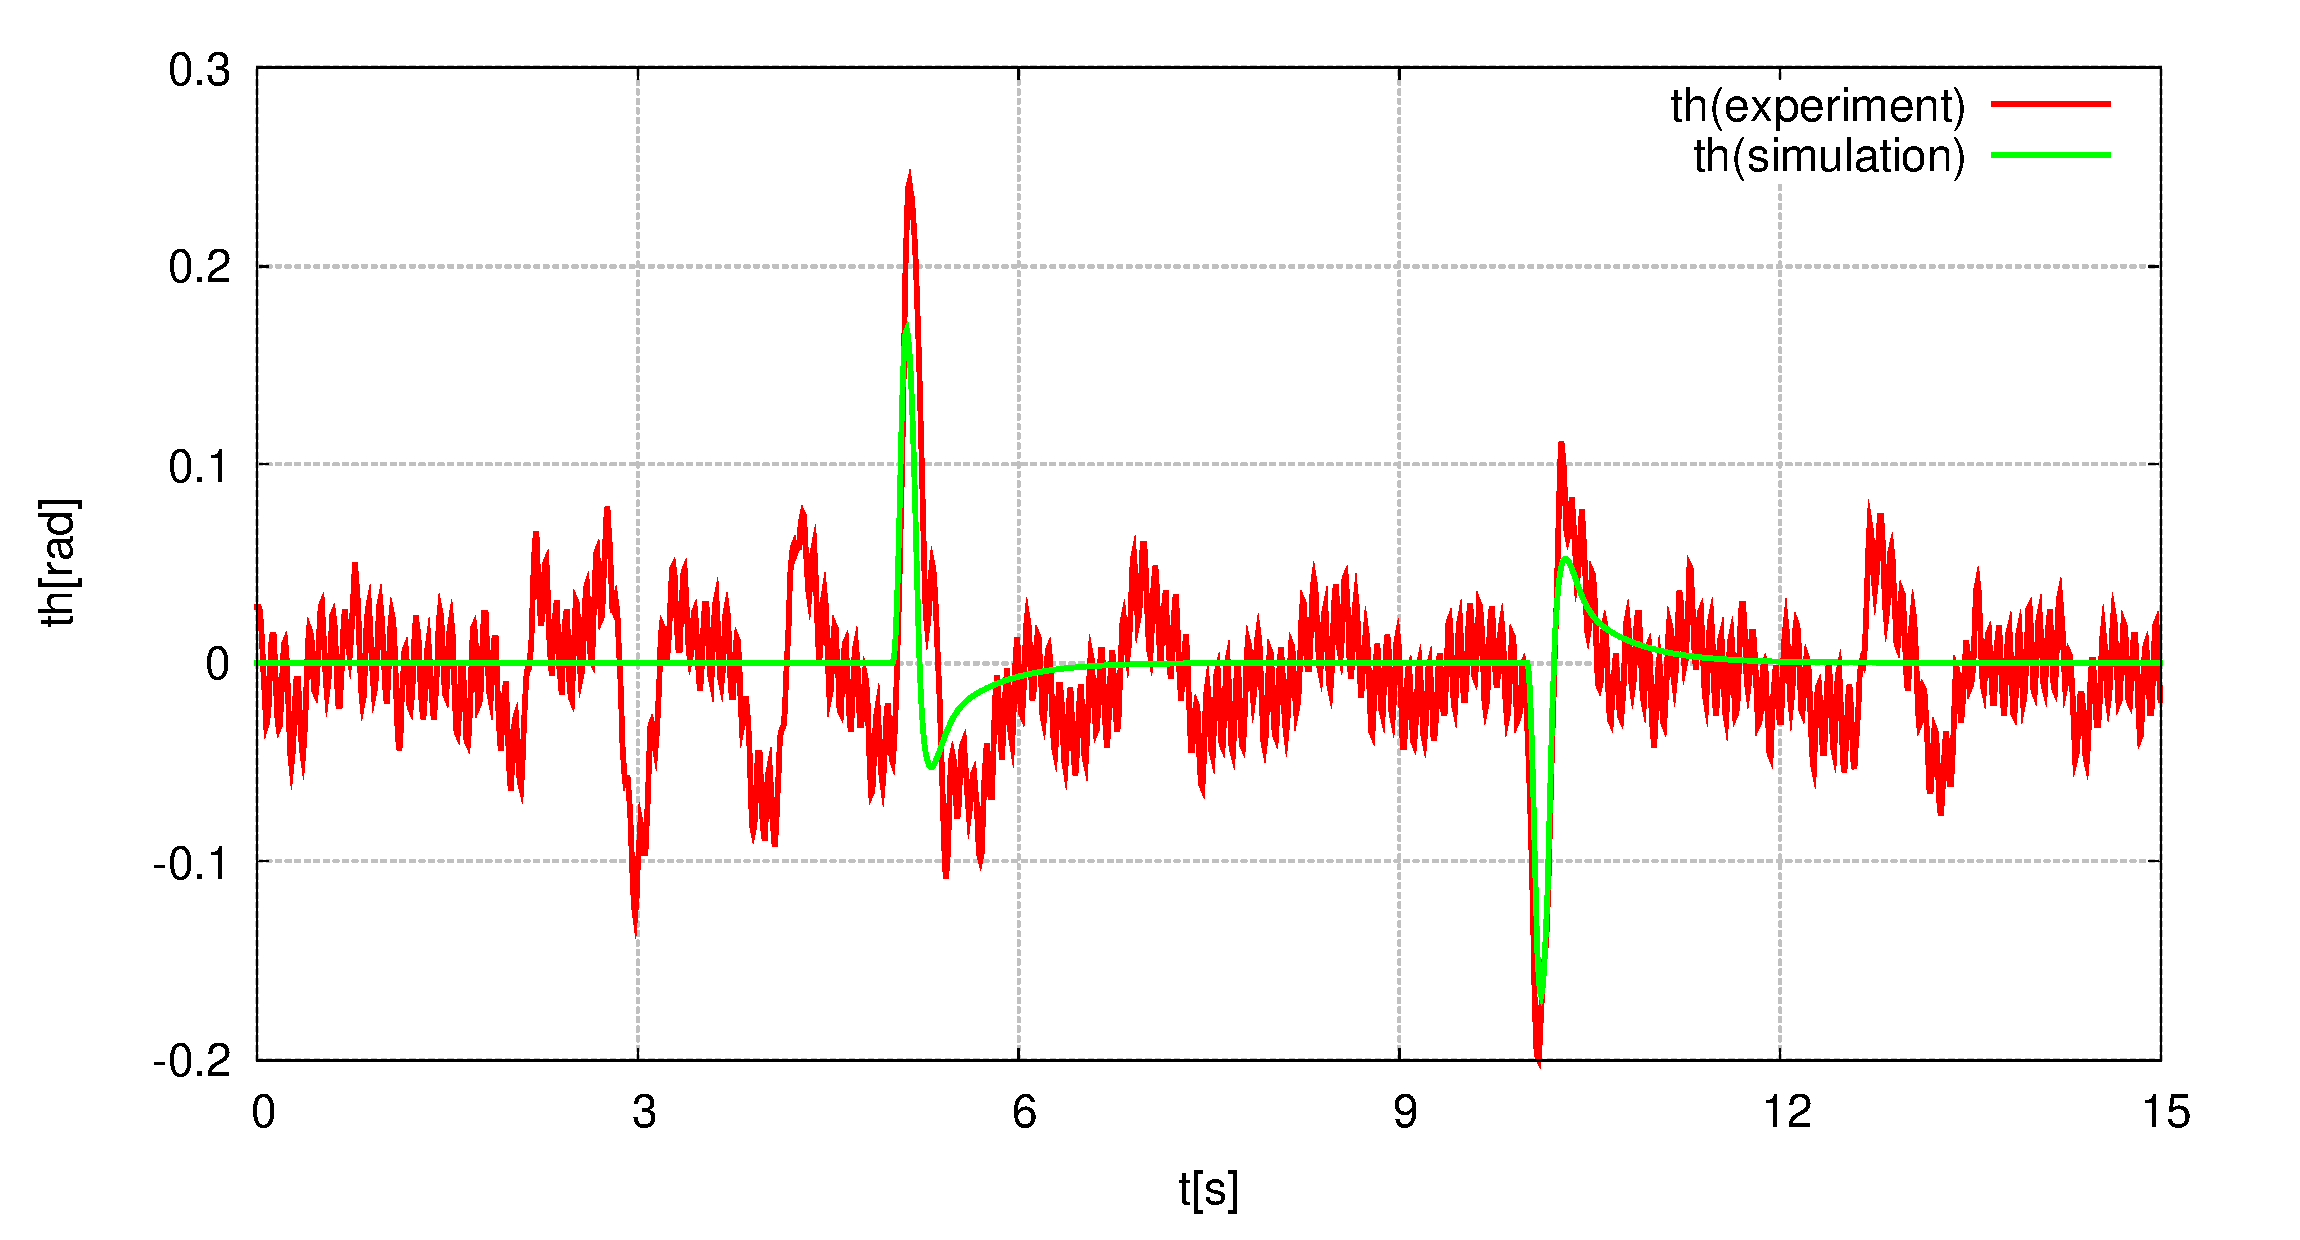
\includegraphics[width=0.49\linewidth]{gazo/experiment_Q65obs60dt10TH2.eps}
		\caption{比較結果その12(左図がr,右図が$\theta$)}
		\label{image:sono12}
	\end{figure}
	以上の図を見てみるとすべての図においてノイズがひどいが、比較的シミュレーション結果と一致している図とまったく一致していない図があるのが分かる。
	前者に当てはまる図は図\ref{image:sono1}、図\ref{image:sono3}、図\ref{image:sono4}、図\ref{image:sono6}
	、図\ref{image:sono7}、図\ref{image:sono9}、図\ref{image:sono12}。後者に当てはまる図は、
	図\ref{image:sono2}、図\ref{image:sono5}、図\ref{image:sono8}、図\ref{image:sono11}である。
	後者に共通する特徴は重み行列が$\rm{diag}(1E5,1E6,1,1)$となっている点である。
	このようにしたときの特徴としてはシミュレーションの章でも述べたが、大きくした成分に対応する状態の応答がよくなるというものであった。
	つまり、この重み行列のとき$\theta$の応答がよくなりるはずである。
	だが、実際の図を見てみると$\theta$の応答はシミュレーションと比較しても一致しているとは言えない。
	また、$r$に関しては図を見る限りでは目標値変更ができていないといえる。
	これは、重み行列をこうしたことで$r$の応答は遅くなったためといえる。
	普通であれば、プログラムが5秒おきに目標値を変更するので、台車はその目標値に向かって動き出す。
	しかし、$r$の応答が遅いため台車は目標値に到達することができずに、プログラムから次の目標値が入力される。
	こうなってしまうことで台車は常に動き続けている状態になり、応答が良くなるはずの$\theta$もそれに伴い
	悪くなるといえる。そのため、$r$は目標値に追従できず、$\theta$の応答も悪くなるといえる。
	\par
	シミュレーションと実験において差異がでたが目標値変更を行っての安定化制御を行うことができたので
	実験目的の第二項目は達成できたといえる。
	
	

%-----------------------------------------------------------
\newpage
\section{振り上げ制御及び安定化実験}
	振子を真下に配置し、そこから台車の動きだけで振子を振り上げ、
	安定化制御が可能か実験を行う(実験項目の第三項目)。
	以下に$k$を変更したときの実験結果を示す。
	\begin{figure}[H]
		\centering
		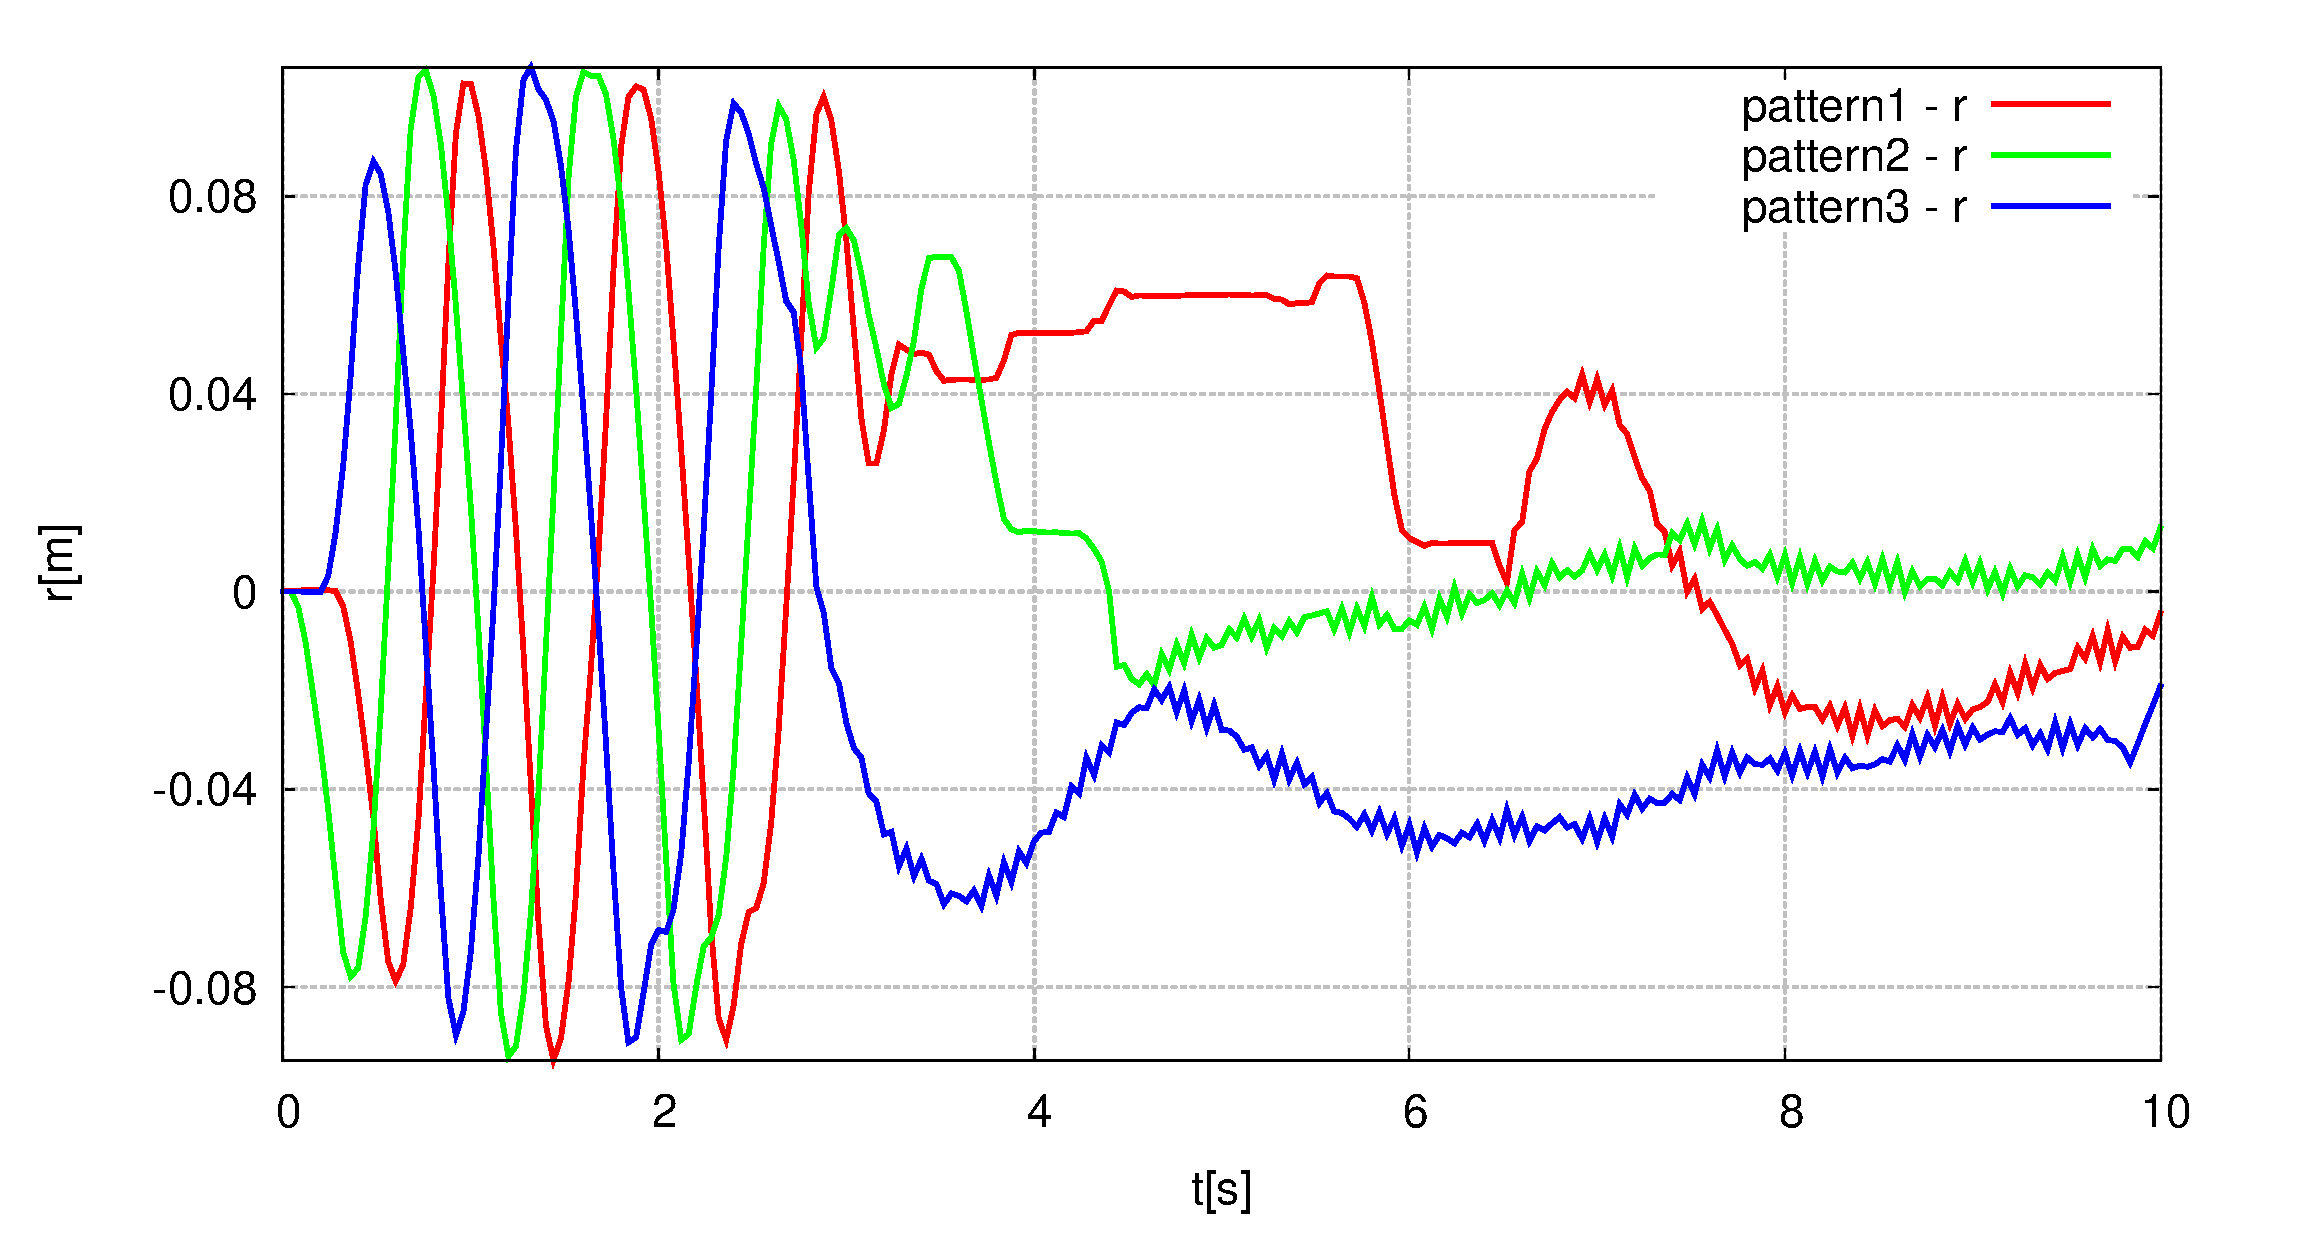
\includegraphics[width=0.49\linewidth]{gazo/Hexpe_R.eps}
		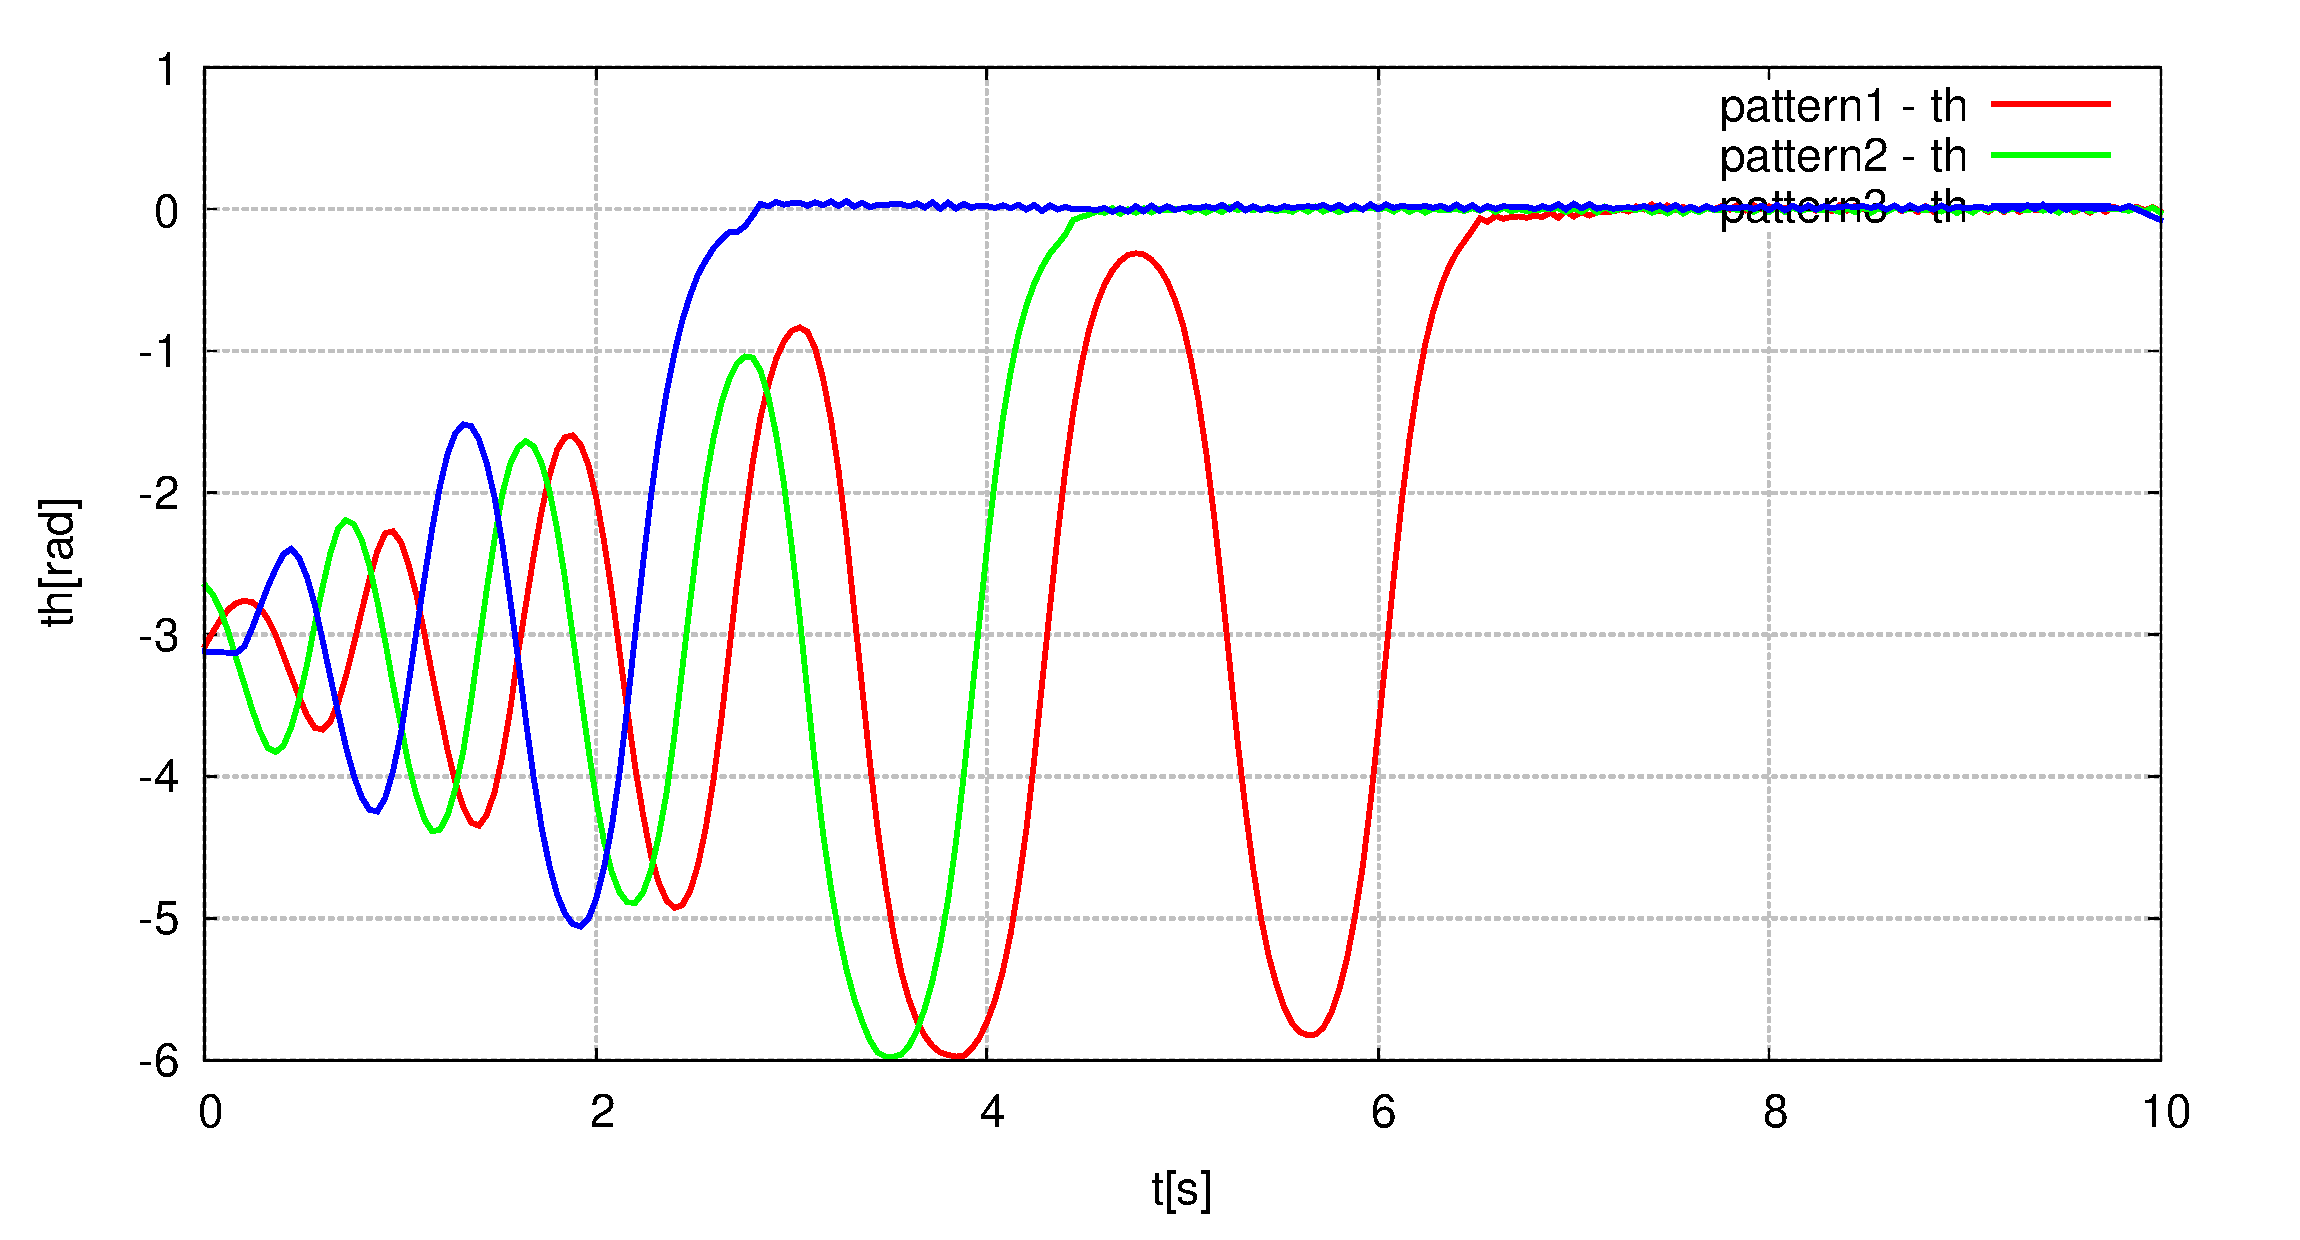
\includegraphics[width=0.49\linewidth]{gazo/Hexpe_TH.eps}
		\caption{$k$の違いによる実験結果の比較}
		\label{image:Hexpe}
	\end{figure}
	図中のPatternは以下の表に対応するパラメータである。
	\begin{table}[H]
		\begin{center}
			\caption{実験に用いたパラメータの組}
			\medskip
			
			\begin{tabular}{|c|c|c|}\hline
				& $n$ & $k$ \\ \hline\hline
				パターン1 & 0.4 & $1.0×10^3$  \\ \hline
				パターン2 & 0.4 & $1.0×10^4$  \\ \hline
				パターン3 & 0.4 & $1.0×10^5$  \\ \hline
			\end{tabular}
		\end{center}
		\label{table:huriage_huriage}
	\end{table}
	図\ref{image:Hexpe}の右図より、$k$の値が大きいほど早く安定化制御に移行していることがわかる。
	$k$が大きくなるとエネルギーの収束が早くなるため、より早く安定化制御に移行できたといえる。
	つまり、シミュレーションの章で行った考察は間違っていたということになる。これは、実験に用いた
	倒立振子系のシミュレーションを行う際に考慮すべき項目が抜けていたか、同定した倒立振子系のパラメータが
	間違っていたかなど様々な原因が考えられる。
	以下に実験結果とシミュレーション結果との比較を行った図を示す。
	\begin{figure}[H]
		\centering
		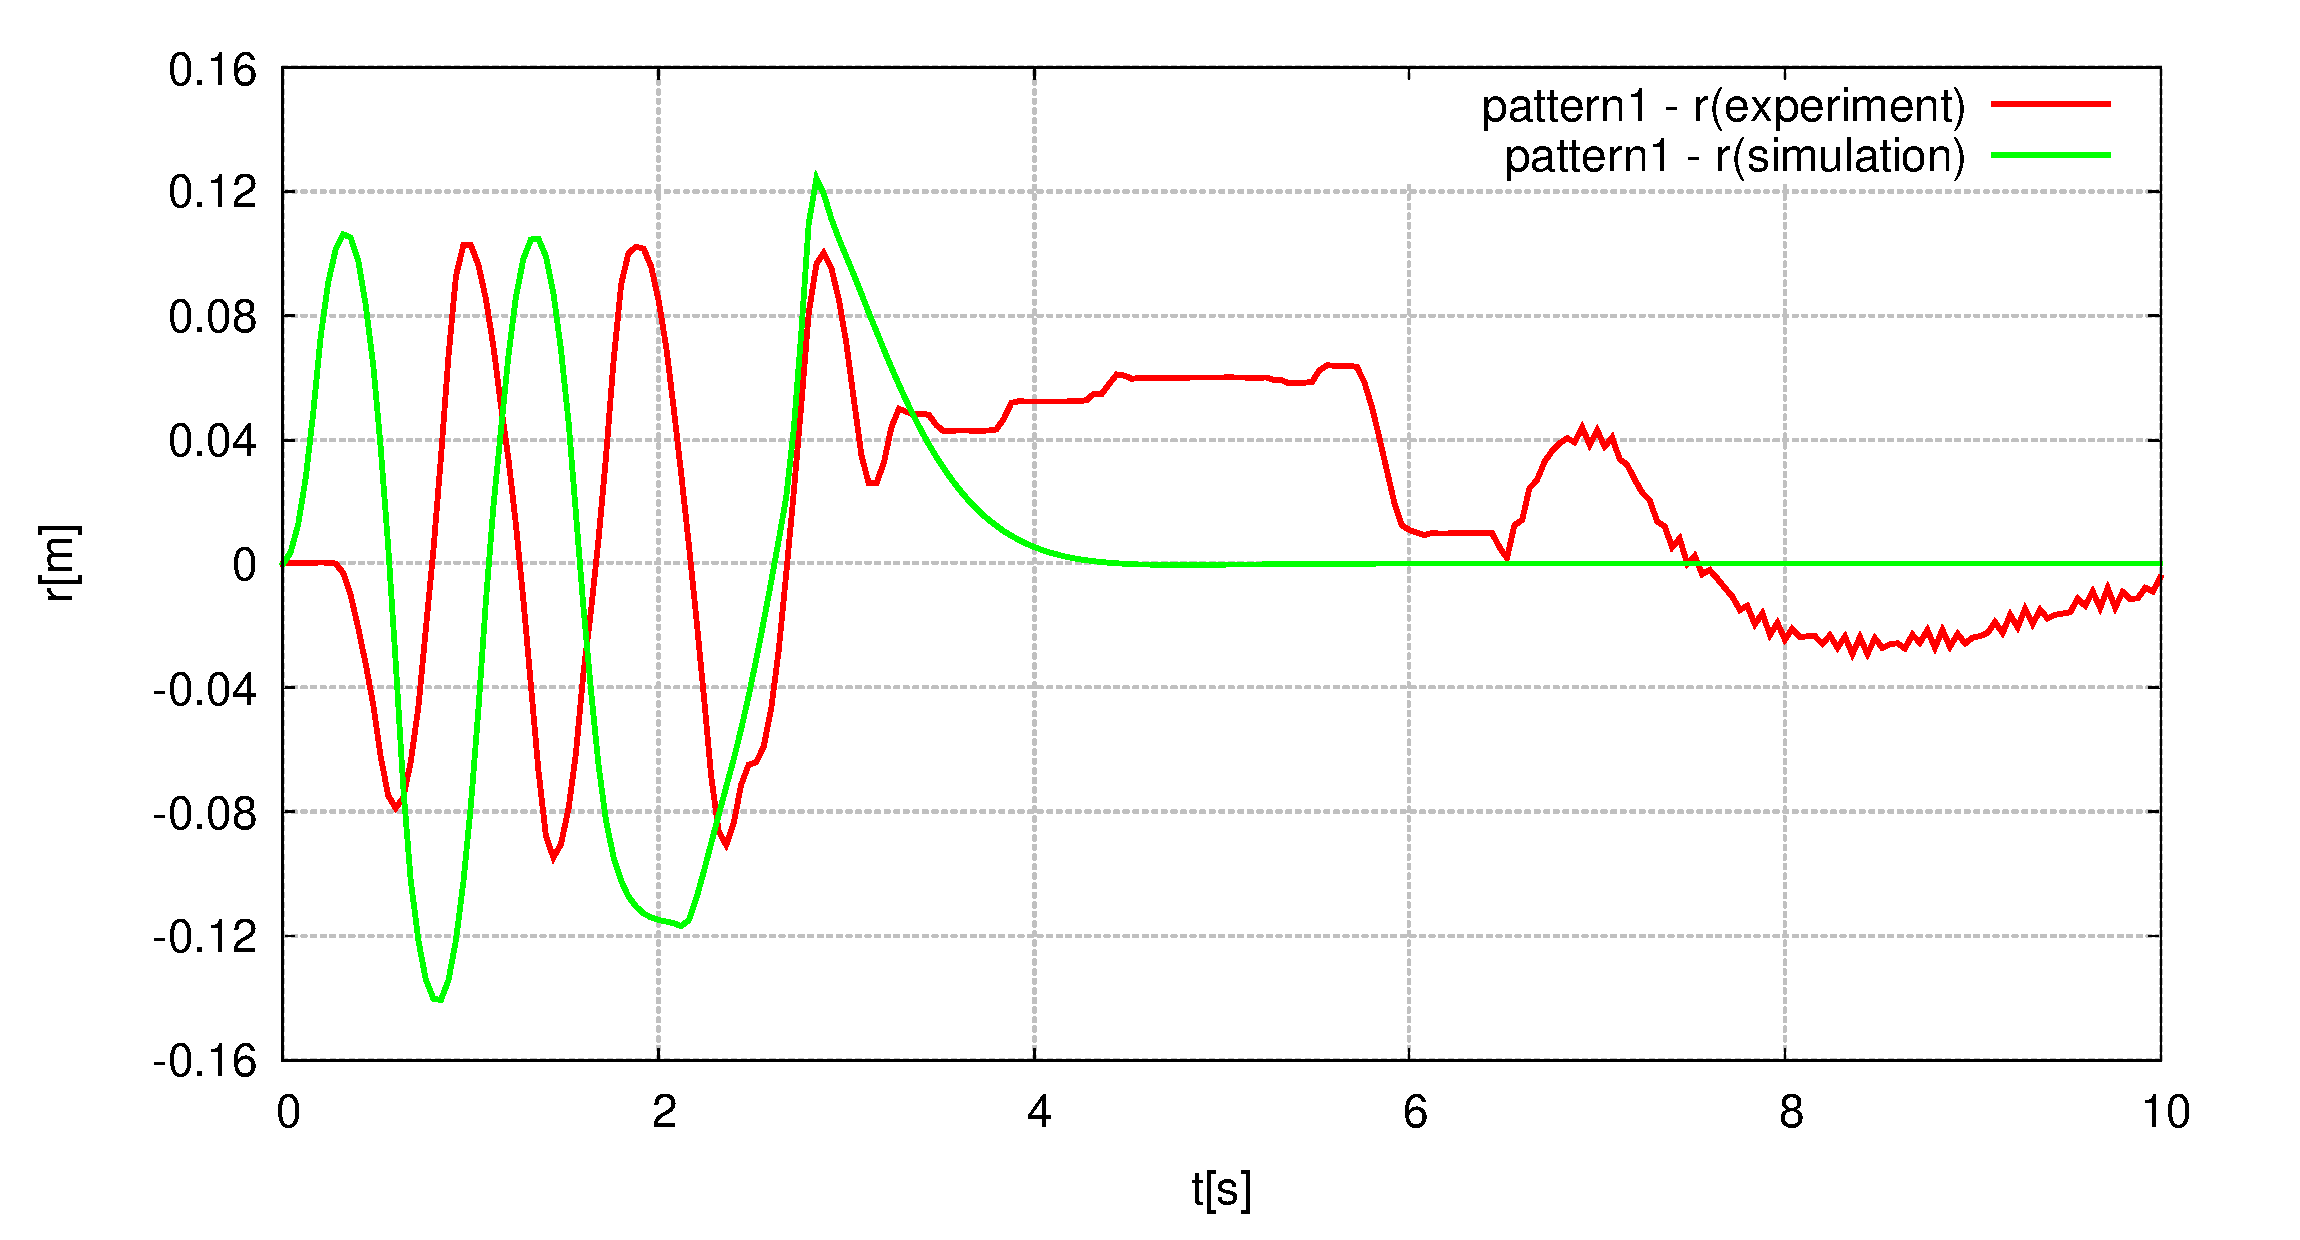
\includegraphics[width=0.49\linewidth]{gazo/HcompP1R.eps}
		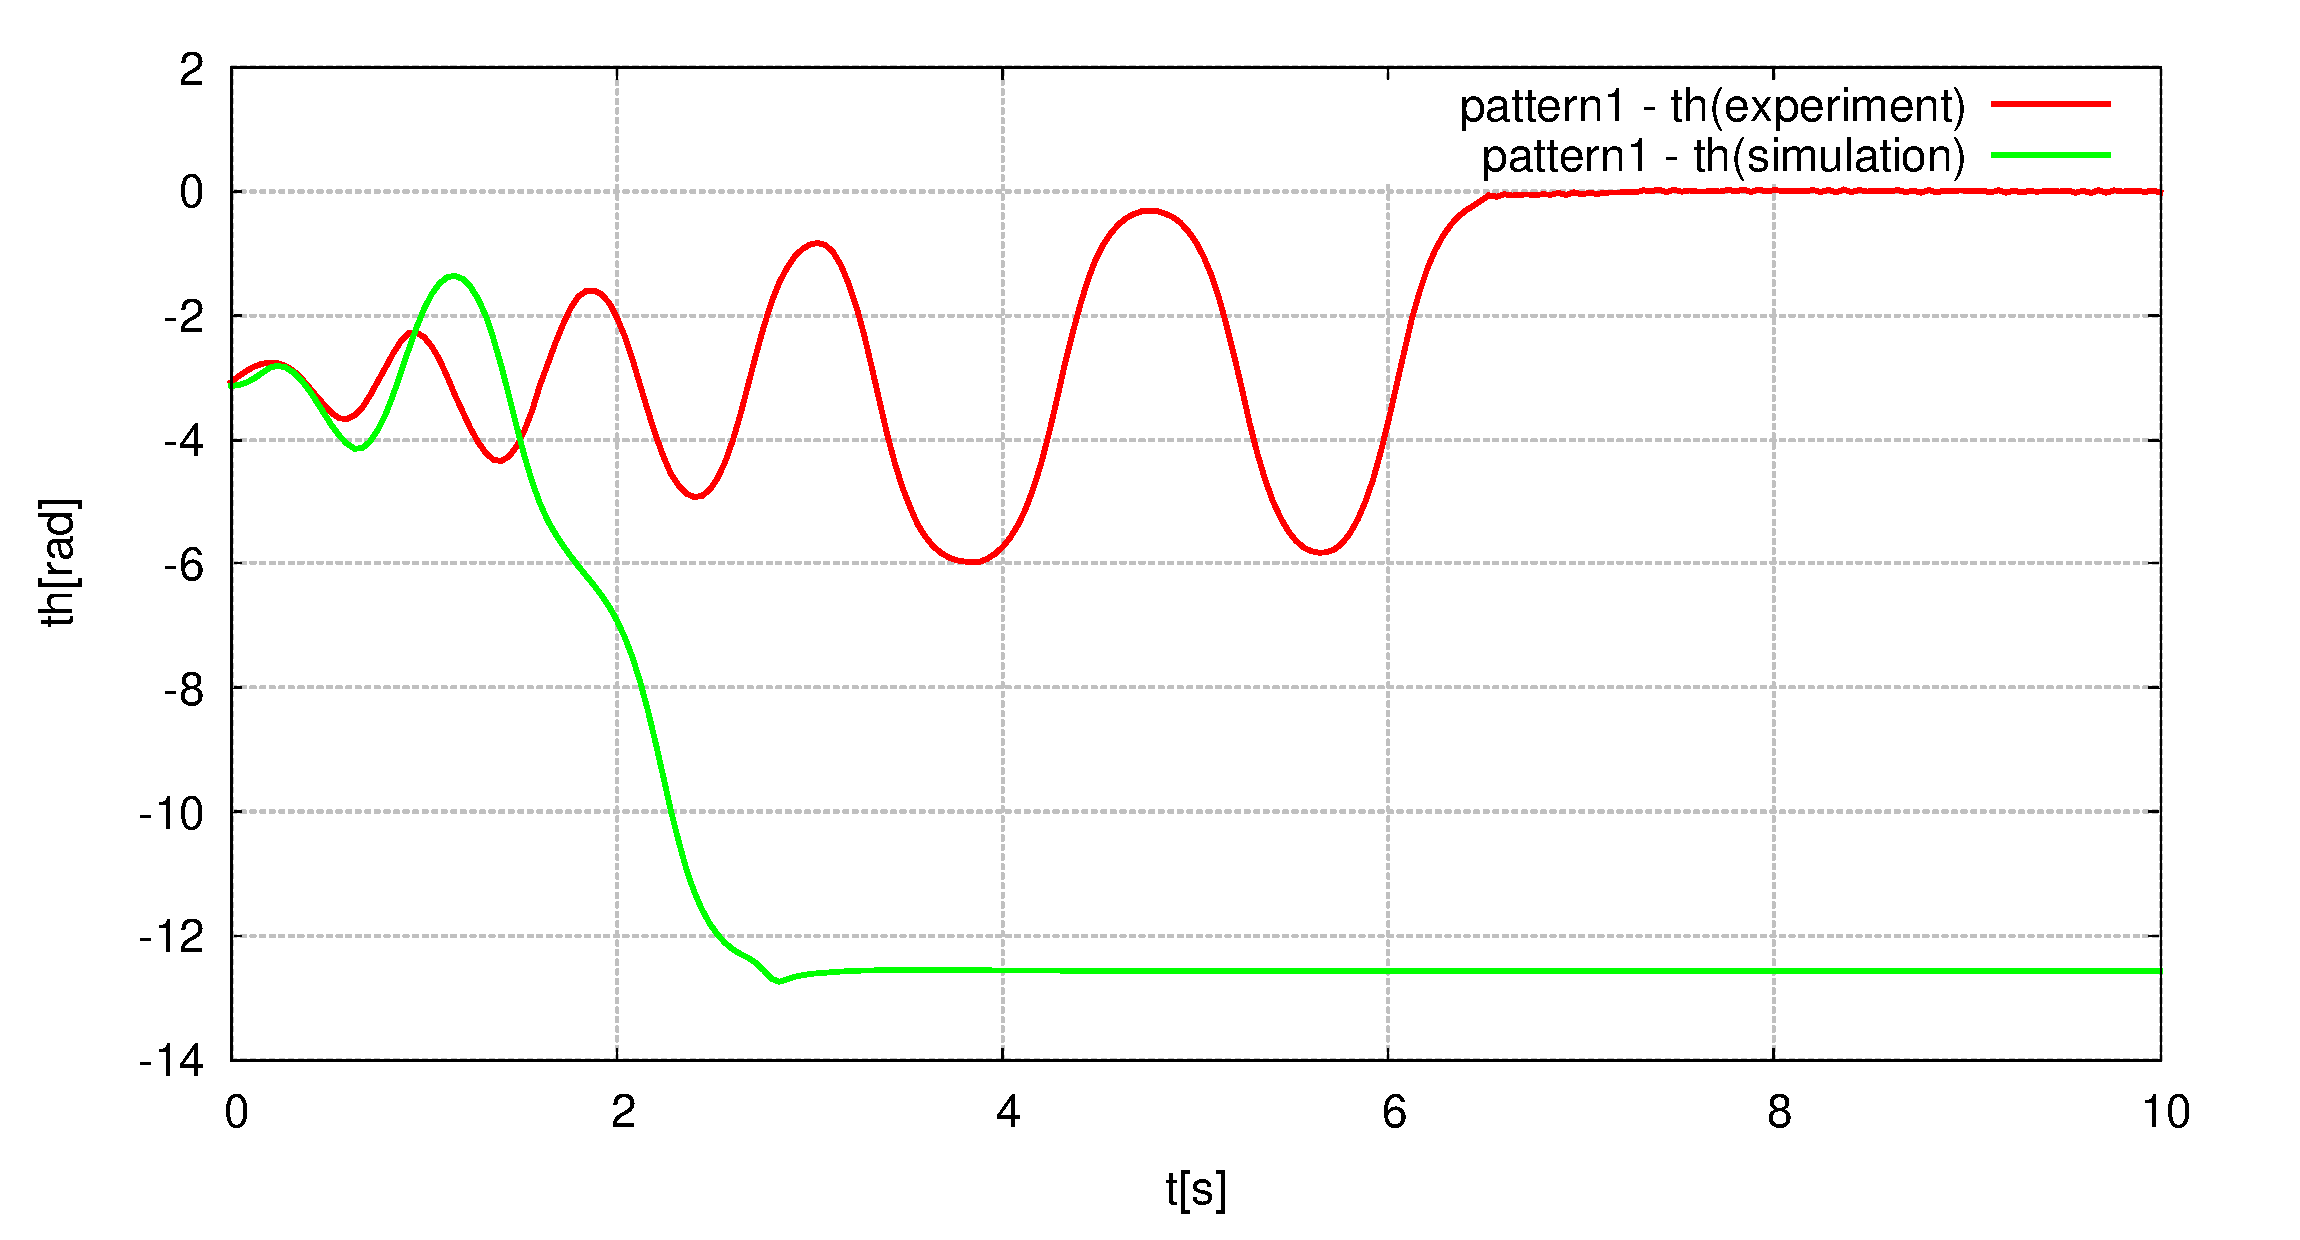
\includegraphics[width=0.49\linewidth]{gazo/HcompP1TH.eps}
		\caption{比較結果(Pattern1)}
		\label{image:HcompP1}
	\end{figure}
	\begin{figure}[H]
		\centering
		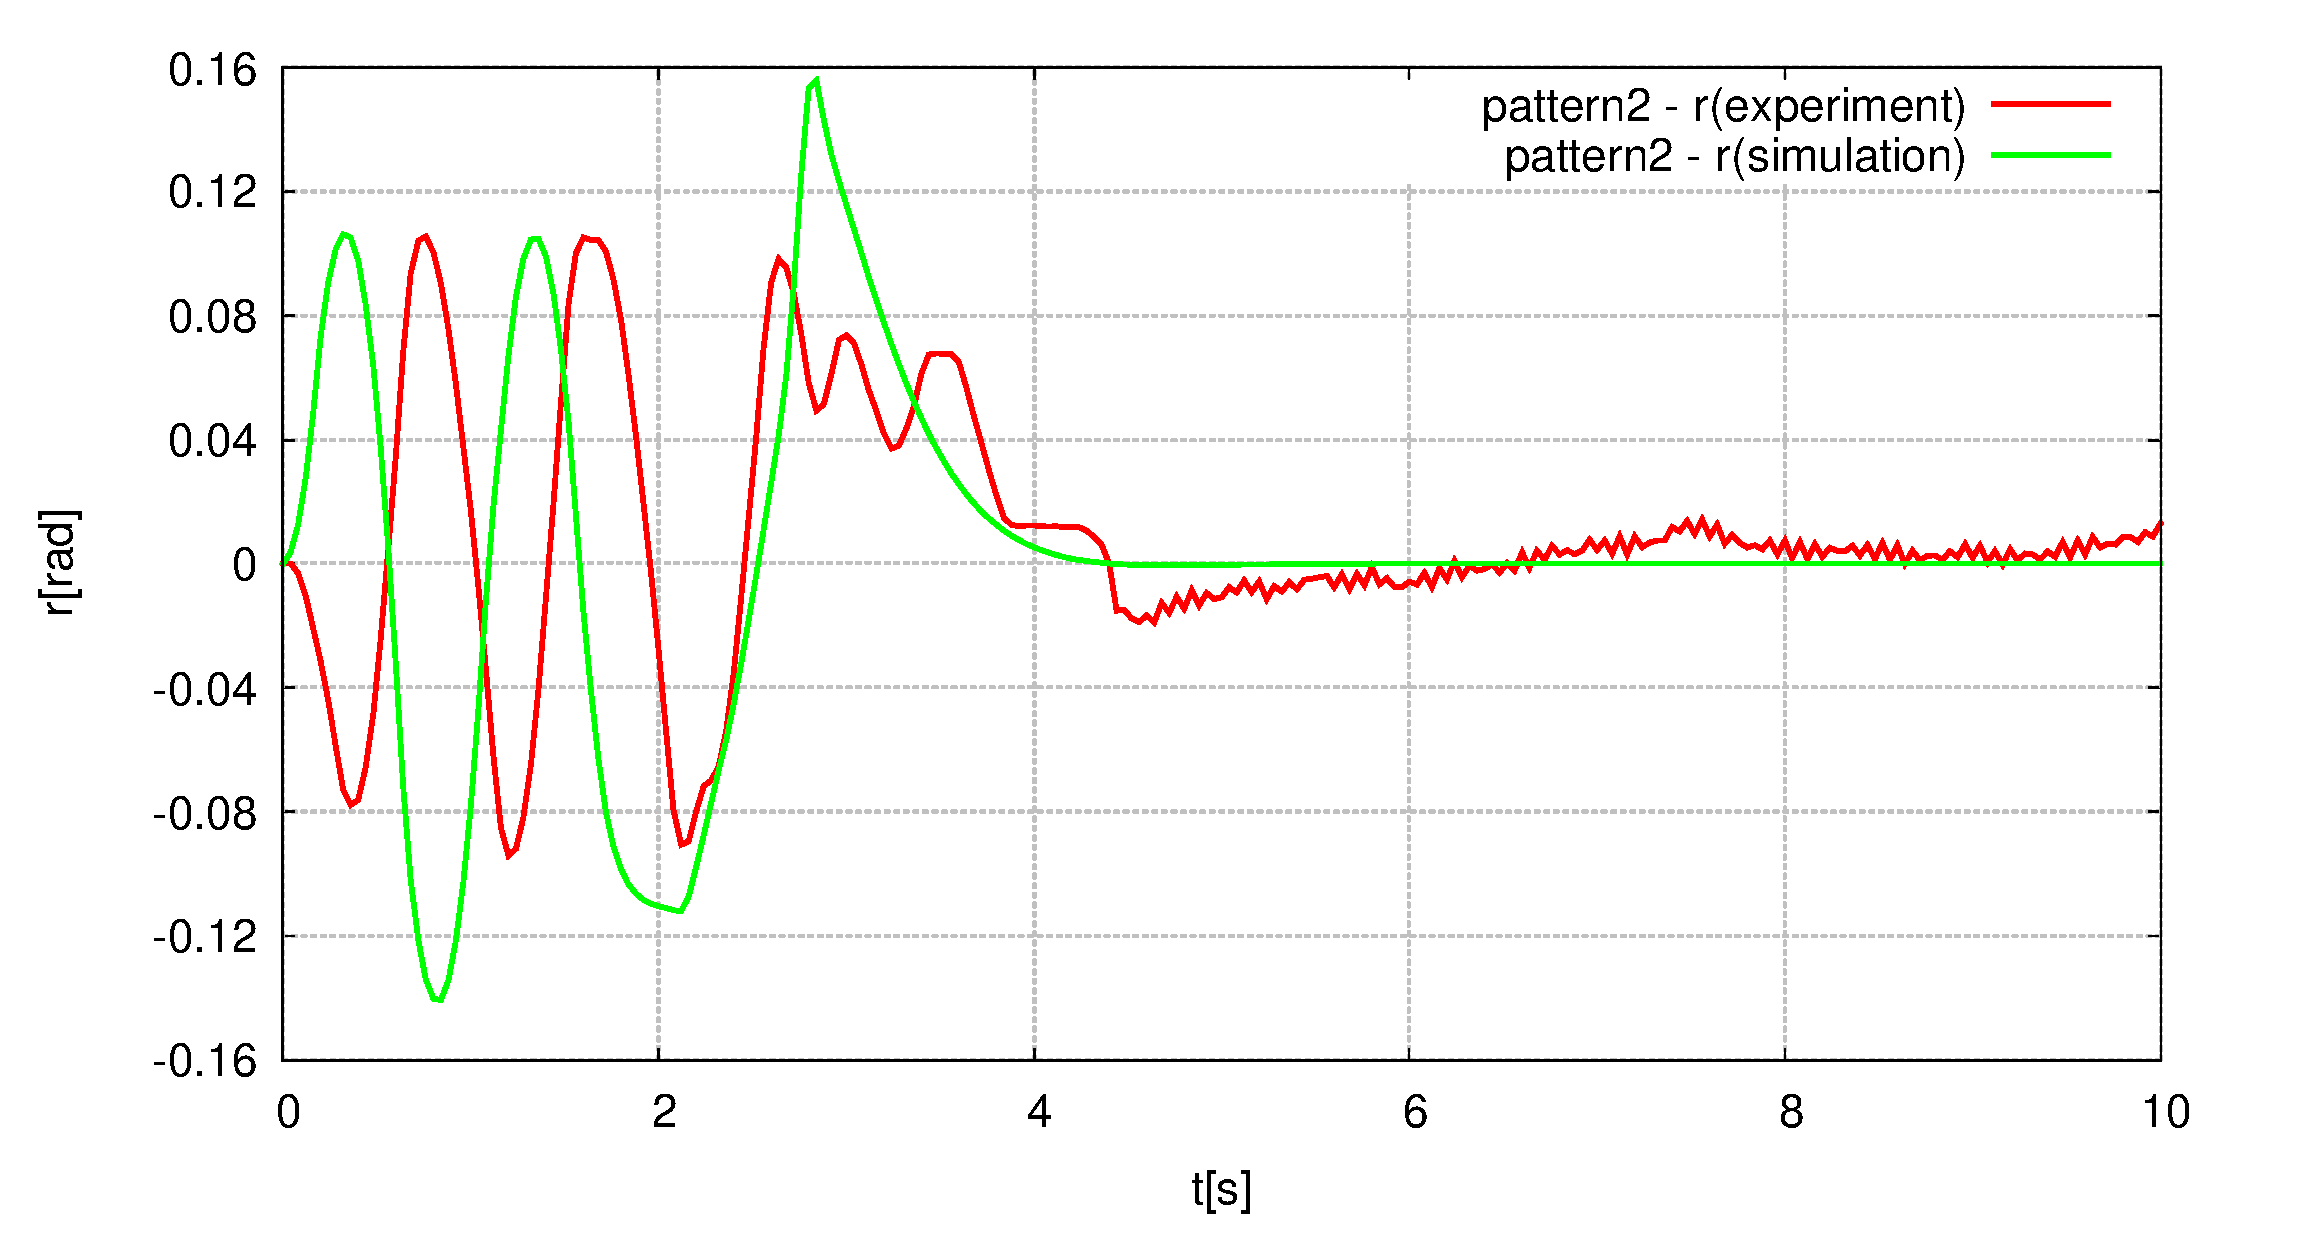
\includegraphics[width=0.49\linewidth]{gazo/HcompP2R.eps}
		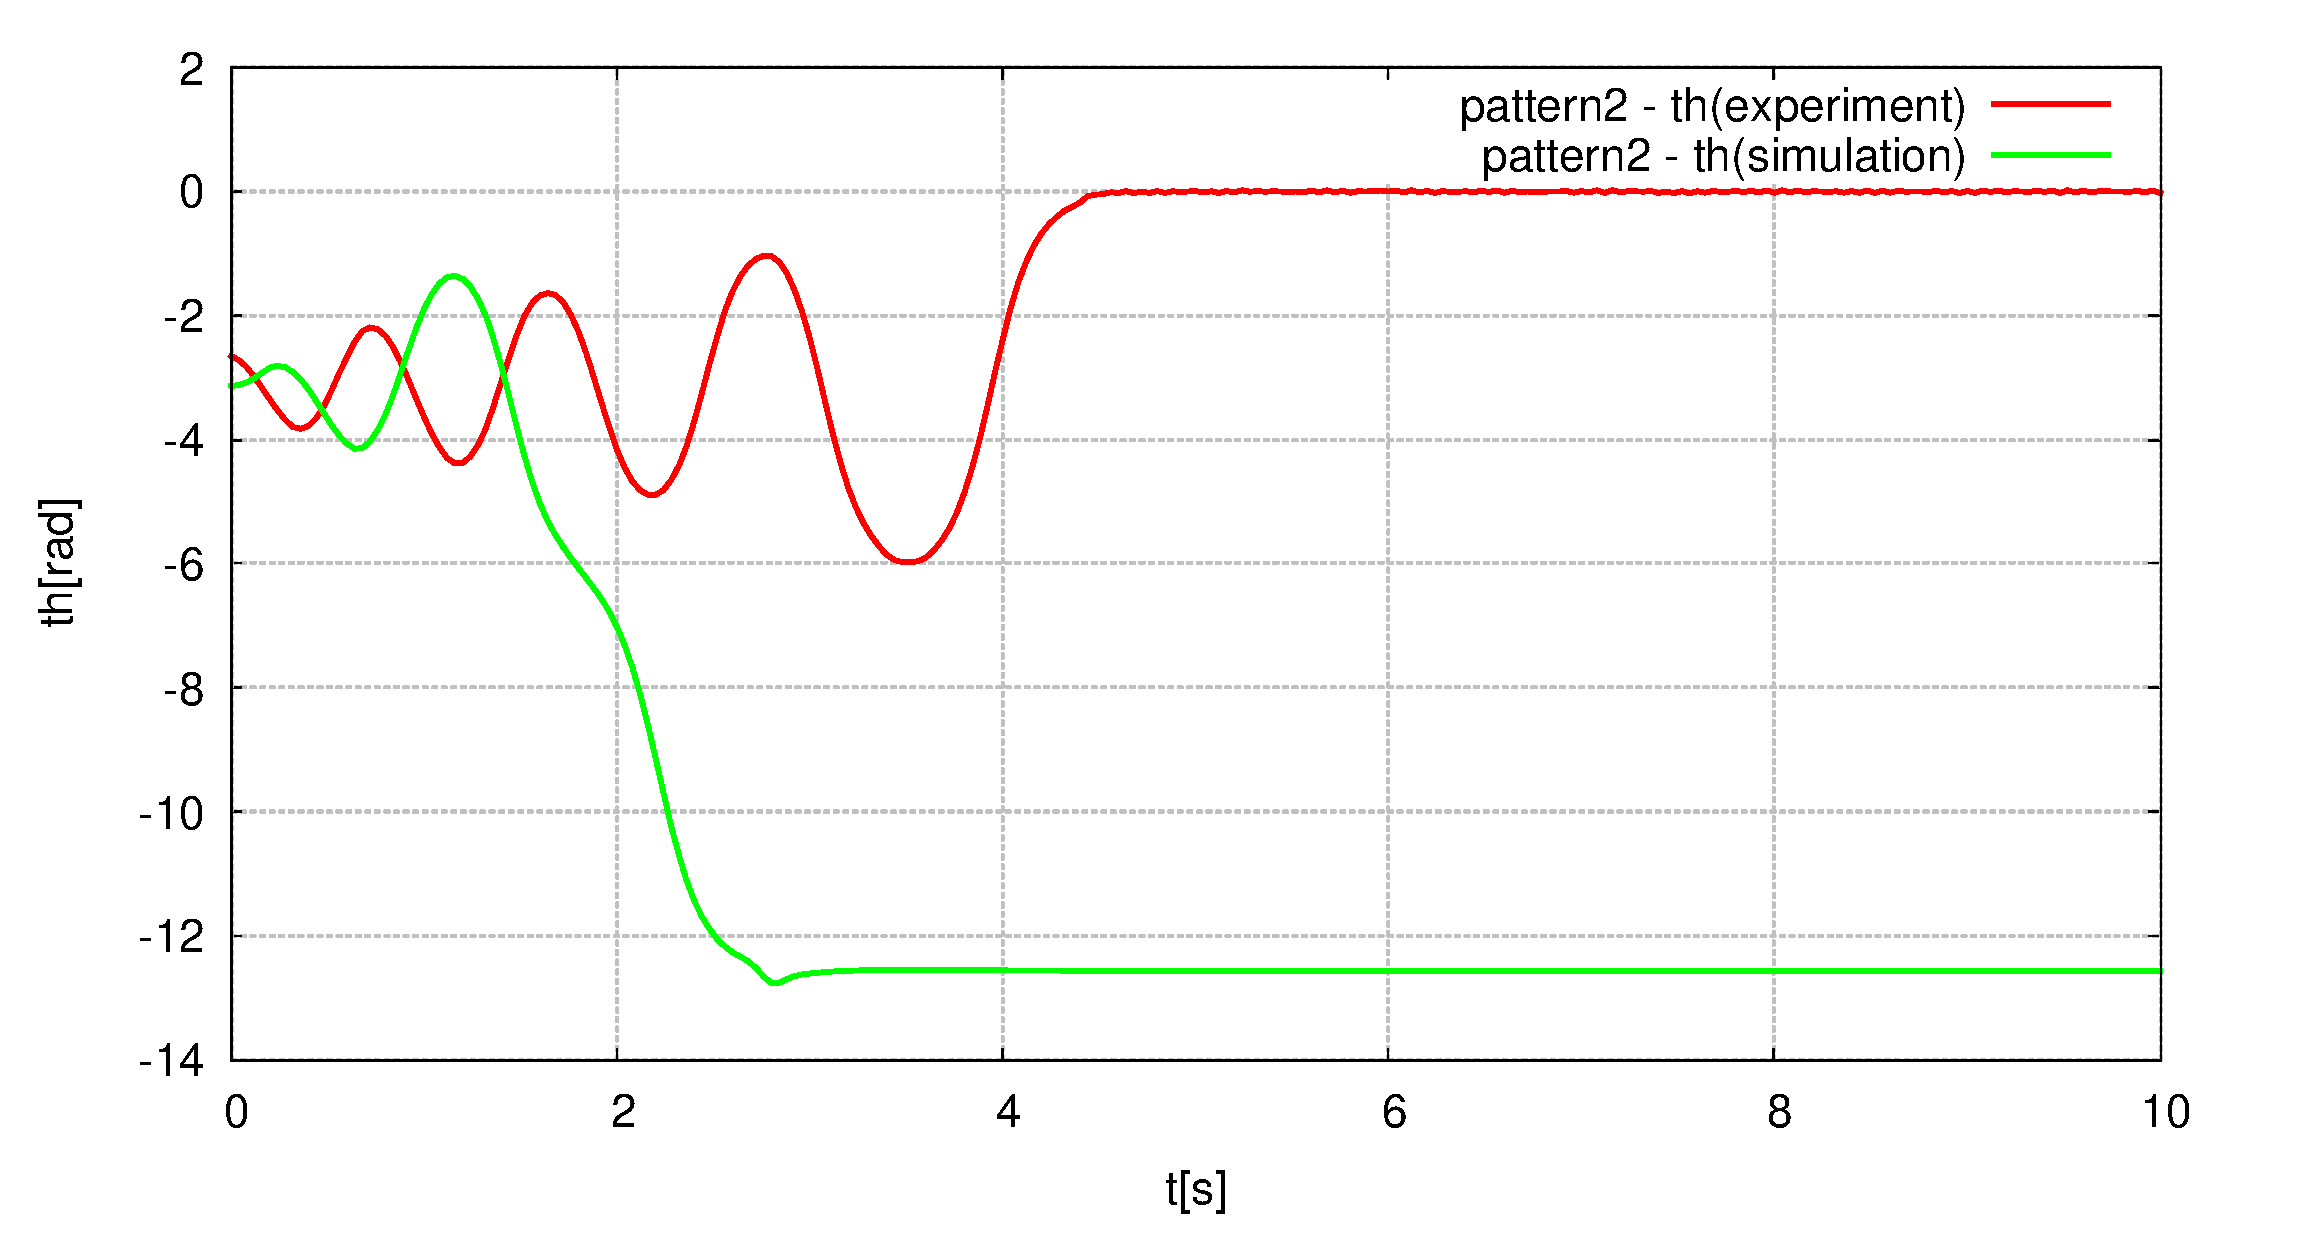
\includegraphics[width=0.49\linewidth]{gazo/HcompP2TH.eps}
		\caption{比較結果(Pattern2)}
		\label{image:HcompP2}
	\end{figure}
	\begin{figure}[H]
		\centering
		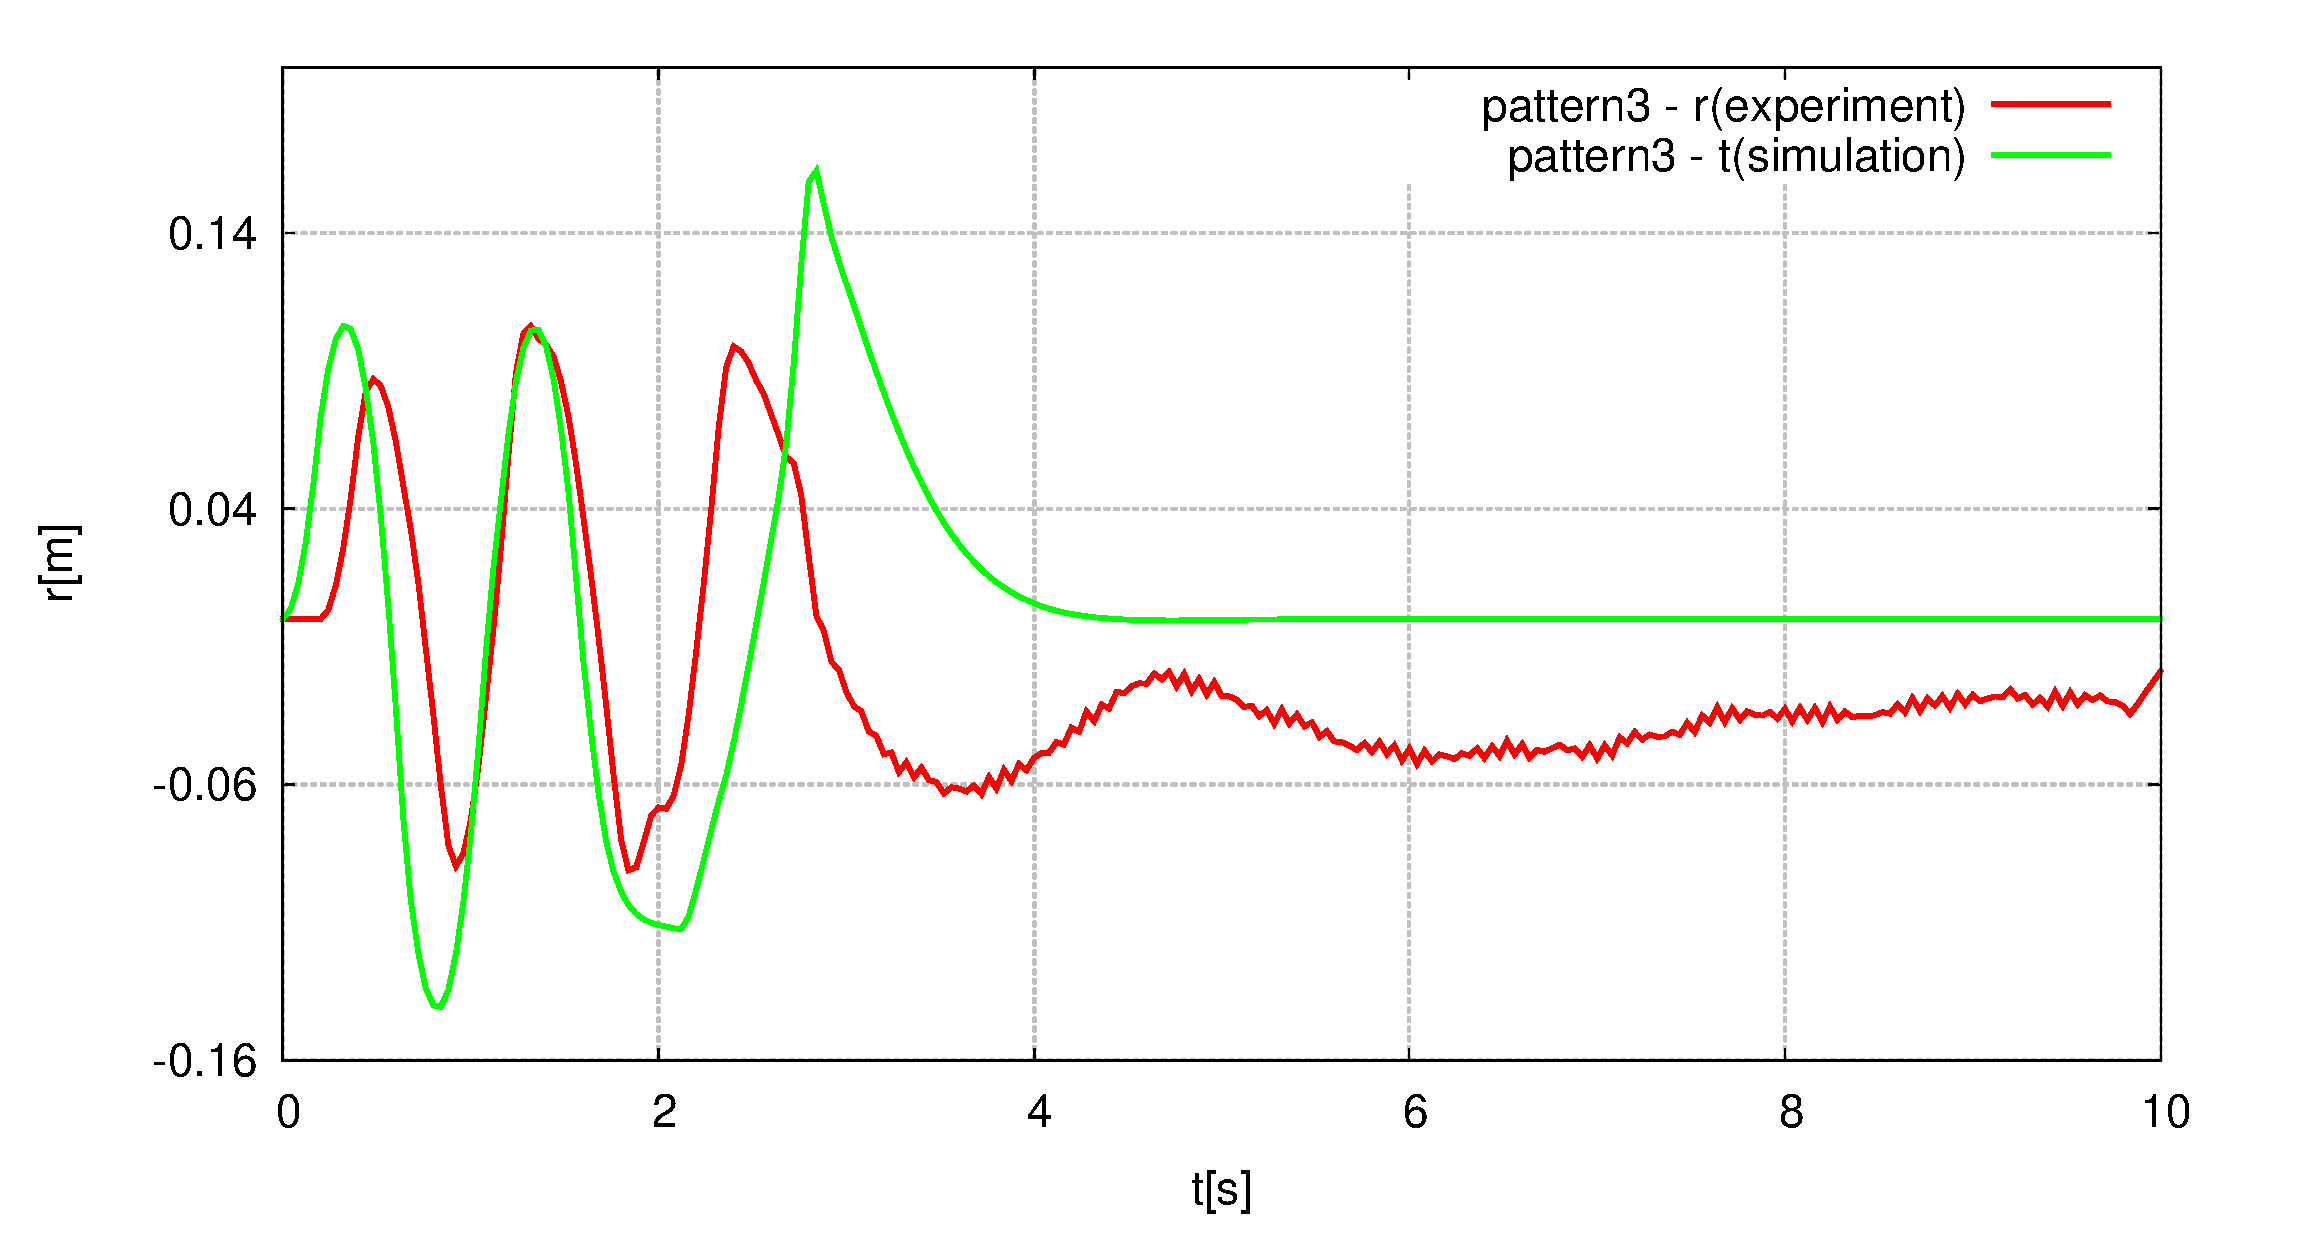
\includegraphics[width=0.49\linewidth]{gazo/HcompP3R.eps}
		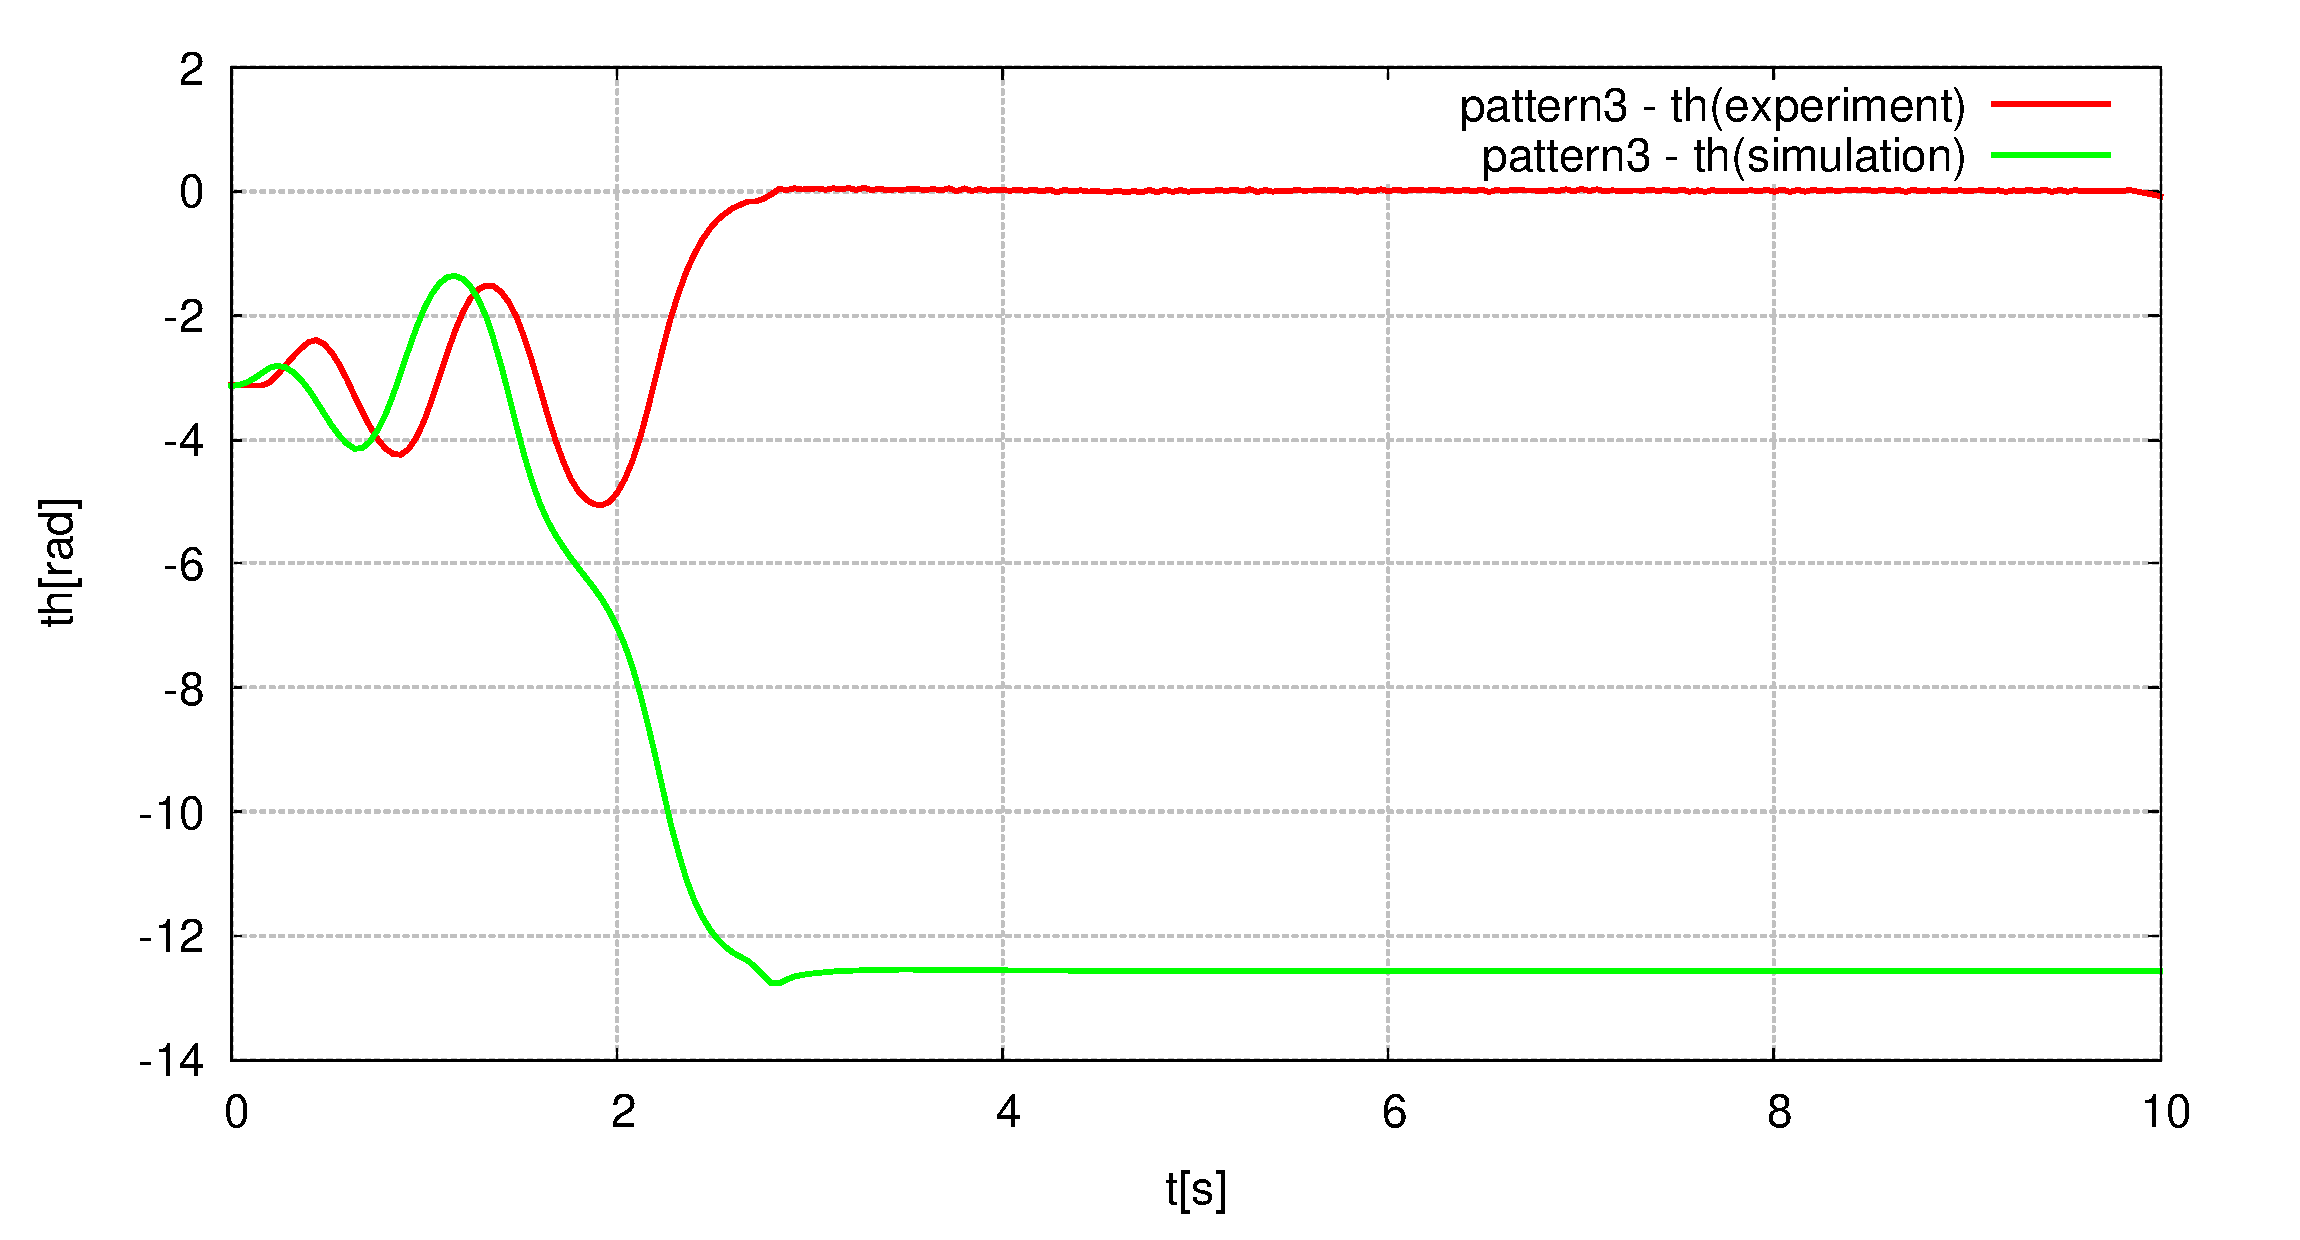
\includegraphics[width=0.49\linewidth]{gazo/HcompP3TH.eps}
		\caption{比較結果(Pattern3)}
		\label{image:HcompP3}
	\end{figure}
	
	\par
	シミュレーションの結果と実験の結果に大きな違いが出てしまったが、
	実験において振り上げ制御から安定化制御を行うことができたので、
	実験目的の第三項目を達成できたといえる。
	
%-----------------------------------------------------------